\documentclass[a4paper,11pt,fleqn,dvipsnames,twoside,openright,sort&compress]{memoir} 	% Openright aabner kapitler paa hoejresider (openany begge)

%%%% PACKAGES %%%%

% ¤¤ Oversaettelse og tegnsaetning ¤¤ %
\usepackage[utf8]{inputenc}					% Input-indkodning af tegnsaet (UTF8)
\usepackage[british, danish]{babel}					% Dokumentets sprog
\usepackage[T1]{fontenc}					% Output-indkodning af tegnsaet (T1)
\usepackage{ragged2e,anyfontsize}			% Justering af elementer
\usepackage{nomencl}
\makenomenclature
\usepackage{indentfirst}

% ¤¤ Figurer og tabeller (floats) ¤¤ %
% Tilføjet:
\usepackage{tabularx}
\usepackage{longtable}
\usepackage{graphicx}
\usepackage{pdfpages}
%Linjeskift i tabeller:
\newcommand{\specialcell}[2][c]{%
  \begin{tabular}[#1]{@{}c@{}}#2\end{tabular}}

  %anvend: \specialcell[]{Første del\\ anden del} [t]= align top, [b]= align bottom


% Tyk horisontallinje til tabeller :
\makeatletter
\newcommand{\thickhline}{%
    \noalign {\ifnum 0=`}\fi \hrule height 1.5pt
    \futurelet \reserved@a \@xhline
}
\newcolumntype{"}{@{\hskip\tabcolsep\vrule width 2pt\hskip\tabcolsep}}
\makeatother

% Anvend : \thickhline

\usepackage{tabulary}
\usepackage{graphicx} 						% Haandtering af eksterne billeder (JPG, PNG, EPS, PDF)
\usepackage{wrapfig}
%\usepackage{eso-pic}						% Tilfoej billedekommandoer paa hver side
%\usepackage{wrapfig}						% Indsaettelse af figurer omsvoebt af tekst. \begin{wrapfigure}{Placering}{Stoerrelse}
\usepackage{multirow}                		% Fletning af raekker og kolonner (\multicolumn og \multirow)
\usepackage{multicol}         	        	% Muliggoer output i spalter
\usepackage{rotating}						% Rotation af tekst med \begin{sideways}...\end{sideways}
\usepackage{colortbl} 						% Farver i tabeller (fx \columncolor og \rowcolor)
\usepackage{xcolor}							% Definer farver med \definecolor. Se mere: http://en.wikibooks.org/wiki/LaTeX/Colors
\usepackage{flafter}						% Soerger for at floats ikke optraeder i teksten foer deres reference
\let\newfloat\relax 						% Justering mellem float-pakken og memoir
\usepackage{float}							% Muliggoer eksakt placering af floats, f.eks. \begin{figure}[H]

\graphicspath{{billeder/}}						% Sti til figure

% ¤¤ Matematik mm. ¤¤
\usepackage{amsmath,amssymb,stmaryrd} 		% Avancerede matematik-udvidelser
\usepackage{mathtools}						% Andre matematik- og tegnudvidelser
\usepackage{textcomp}                 		% Symbol-udvidelser (f.eks. promille-tegn med \textperthousand )
\usepackage{amsthm}
\usepackage{rsphrase}						% Kemi-pakke til RS-saetninger, f.eks. \rsphrase{R1}
\usepackage[version=3]{mhchem} 				% Kemi-pakke til flot og let notation af formler, f.eks. \ce{Fe2O3}
\usepackage[binary-units=true, per-mode=fraction]{siunitx}						% Flot og konsistent
\DeclareSIUnit\vote{stemme}
\DeclareSIUnit\votes{stemmer}
%\SI{tal}{enhed}
\sisetup{output-decimal-marker = {,}}		% Opsaetning af \SI (DE for komma som decimalseparator)
\usepackage{icomma}							% Komma som decimal operator

% ¤¤ Referencer og kilder ¤¤ %
\usepackage[danish, english]{varioref}				% Muliggoer bl.a. krydshenvisninger med sidetal (\vref)
\usepackage[numbers]{natbib}							% Udvidelse med naturvidenskabelige citationsmodeller
%\usepackage{xr}							% Referencer til eksternt dokument med \externaldocument{<NAVN>}
%\usepackage{glossaries}					% Terminologi- eller symbolliste (se mere i Daleifs Latex-bog)
% ¤¤ Misc. ¤¤ %
\usepackage{listings}						% Placer kildekode i dokumentet med \begin{lstlisting}...\end{lstlisting}
\usepackage{lipsum}							% Dummy text \lipsum[..]
\usepackage[shortlabels]{enumitem}			% Muliggoer enkelt konfiguration af lister
\usepackage{pdfpages}
\usepackage{pdflscape}					% Goer det muligt at inkludere pdf-dokumenter med kommandoen \includepdf[pages={x-y}]{fil.pdf}
\pdfoptionpdfminorversion=6					% Muliggoer inkludering af pdf dokumenter, af version 1.6 og hoejere
\pretolerance=2500 							% Justering af afstand mellem ord (hoejt tal, mindre orddeling og mere luft mellem ord)

% Kommentarer og rettelser med \fxnote. Med 'final' i stedet for 'draft' udloeser hver note en error i den faerdige rapport.
\usepackage{footnote}
\usepackage[footnote,draft,danish,silent,nomargin]{fixme}
\makesavenoteenv{tabular}


\usepackage[ntheorem]{mdframed} %Bruges for at kunne lave definitionsboksene

\usepackage{filecontents}

%%%% CUSTOM SETTINGS %%%%
%%%%To-do markater%%%%
\usepackage{todonotes}

%%Tikz%%
\usepackage{tikz}
\usepackage{tikz-uml}
\usetikzlibrary{shapes.geometric, arrows, chains, matrix, mindmap, patterns, shapes.misc, trees, positioning}

%rettet fra Emilie%
\tikzstyle{startstop} = [rectangle, ultra thick, rounded corners, minimum width=3cm, minimum height=1cm,text centered, text width=3cm, draw=black, fill=white]
\tikzstyle{io} = [trapezium, trapezium left angle=80, trapezium right angle=80, ultra thick, minimum width=3cm, minimum height=1cm, text centered, draw=black, fill=white]
\tikzstyle{process} = [rectangle, thick, minimum width=1cm, minimum height=0.75cm, text centered, draw=black, fill=white]
\tikzstyle{simple} = [rectangle, minimum width=1cm, minimum height=0.75cm, text centered, fill=white]
\tikzstyle{specialprocess} = [rectangle, ultra thick, minimum width=3cm, minimum height=1cm, text centered, draw=black, fill=white]
\tikzstyle{decision} = [diamond, ultra thick, minimum width=3cm, minimum height=1cm, text centered, draw=black, fill=white]
\tikzstyle{seconddecision} = [circle, ultra thick, minimum width=3cm, minimum height=1cm, text centered, draw=black, fill=white]
\tikzstyle{predefined} = [rectangle, rounded corners, ultra thick, minimum width=3cm, minimum height=1cm,text centered, text width=3cm, draw=black, fill=white]
\tikzstyle{data} = [trapezium, trapezium left angle=60, trapezium right angle=120, ultra thick, minimum width=3cm, minimum height=1cm, text centered, draw=black, fill=white]
\tikzstyle{terminator} = [ellipse, ultra thick, minimum width=3cm, minimum height=1cm, text centered, draw=black, fill=white]
\tikzstyle{arrow} = [->,>=open triangle 90]

\tikzstyle{decision} = [diamond, draw, fill=blue!20,
    text width=4.5em, text badly centered, node distance=3cm, inner sep=0pt]
\tikzstyle{block} = [rectangle, draw, fill=blue!20,
    text width=5em, text centered, rounded corners, minimum height=4em]
\tikzstyle{line} = [draw, -latex']
\tikzstyle{cloud} = [draw, ellipse,fill=red!20, node distance=3cm,
    minimum height=2em]

%PGF%
\usepackage{pgfplots}
\usepgfplotslibrary{patchplots}

%%Boxes%%
\definecolor{theoline}{gray}{0.5}
\definecolor{theocolor}{gray}{0.9}
\definecolor{lemcolor}{gray}{0.97}
\definecolor{defcolor}{RGB}{214,234,218}

\mdfdefinestyle{box}{ % saving some space
skipabove=1.5em plus 0.4em minus 0.6em,
%skipbelow=0.5em plus 0.4em minus 0.2em,
%leftmargin=-7pt, rightmargin=-7pt,
innerleftmargin=3pt,innerrightmargin=7pt, innertopmargin=2pt, innerbottommargin=2pt,
%linewidth=1pt,
%splittopskip=3.2em minus 0.2em,
%splitbottomskip=0.5em plus 0.2em minus 0.1em,
}
\newmdtheoremenv[style=box,linecolor=theoline,backgroundcolor=theocolor]{theorem}{Theorem}[section]
\newmdtheoremenv[style=box,linecolor=theoline,backgroundcolor=lemcolor]{lemma}[theorem]{Lemma}
\newmdtheoremenv[style=box,linecolor=theoline,backgroundcolor=lemcolor]{proposition}[theorem]{Proposition}
\newmdtheoremenv[style=box,linecolor=theoline,backgroundcolor=lemcolor]{corollary}[theorem]{Corollary}



%\newtheorem{theorem}{Theorem}[section]
%\newtheorem{lemma}[theorem]{Lemma}
%\newtheorem{proposition}[theorem]{Proposition}
%\newtheorem{corollary}[theorem]{Corollary}
%\newtheorem{case}{Bevis}[theorem]
%\newtheorem{defn}{Definition}[section]

\renewenvironment{proof}[1][Proof]{\begin{trivlist}
\item[\hskip \labelsep {\bfseries #1}]}{\end{trivlist}}

\newenvironment{definition}[1][Definition]{\begin{trivlist}
\item[\hskip \labelsep {\bfseries #1}]}{\end{trivlist}}

\newenvironment{remark}[1][Remark]{\begin{trivlist}
\item[\hskip \labelsep {\bfseries #1}]}{\end{trivlist}}



\theoremstyle{definition}
\newmdtheoremenv[style=box,linecolor=theoline,backgroundcolor=lemcolor]{defn}[theorem]{Definition}

\newtheorem{eks}[theorem]{Example}
\surroundwithmdframed[
   topline=false,
   rightline=false,
   bottomline=false,
   leftmargin=\parindent,
   skipabove=\medskipamount,
   skipbelow=\medskipamount
]{eks}

\newenvironment{example}[1][Example]{\begin{trivlist}
\item[\hskip \labelsep {\bfseries #1}]}{\end{trivlist}}
\surroundwithmdframed[
   topline=false,
   rightline=false,
   bottomline=false,
   leftmargin=\parindent,
   skipabove=\medskipamount,
   skipbelow=\medskipamount
]{example}

\renewcommand{\qed}{\nobreak \ifvmode \relax \else
      \ifdim\lastskip<1.5em \hskip-\lastskip
      \hskip1.5em plus0em minus0.5em \fi \nobreak
      \vrule height0.75em width0.5em depth0.25em\fi}

% ¤¤ Marginer ¤¤ %
\setlrmarginsandblock{3.5cm}{2.5cm}{*}		% \setlrmarginsandblock{Indbinding}{Kant}{Ratio}
\setulmarginsandblock{2.5cm}{3.0cm}{*}		% \setulmarginsandblock{Top}{Bund}{Ratio}
\checkandfixthelayout 						% Oversaetter vaerdier til brug for andre pakker

%	¤¤ Afsnitsformatering ¤¤ %
\setlength{\parindent}{3mm}           		% Stoerrelse af indryk
\setlength{\parskip}{3mm}          			% Afstand mellem afsnit ved brug af double Enter
\linespread{1,1}							% Linie afstand

% ¤¤ Litteraturlisten ¤¤ %
%\bibpunct[,]{[}{]}{;}{a}{,}{,} 				% Definerer de 6 parametre ved Harvard henvisning (bl.a. parantestype og seperatortegn)
\bibliographystyle{unsrtnat}			% Udseende af litteraturlisten.

% ¤¤ Indholdsfortegnelse ¤¤ %
\setsecnumdepth{subsubsection}		 			% Dybden af nummerede overkrifter (part/chapter/section/subsection)
\maxsecnumdepth{subsubsection}					% Dokumentklassens graense for nummereringsdybde
\settocdepth{subsection} 					% Dybden af indholdsfortegnelsen

% ¤¤ Lister ¤¤ %
\setlist{
  topsep=0pt,								% Vertikal afstand mellem tekst og listen
  itemsep=-1ex,								% Vertikal afstand mellem items
}

% ¤¤ Visuelle referencer ¤¤ %
\usepackage[colorlinks,
            pdftex,
            pdfauthor={Andreas Madsen, Anja Nielsen, Anna Bonde, Astrid Ipsen, Henrik Christensen, Rasmus Kjær og Taniya Henriksen},
            pdftitle={Fanciful Handbook Management},
            pdfsubject={Developing a Handbook Management System for SMBs},
            pdfkeywords={handbooks,document,compsci},
            pdfproducer={Latex with hyperref},
            pdfcreator={pdflatex, or other tool}]{hyperref}			% Danner klikbare referencer (hyperlinks) i dokumentet.
\hypersetup{colorlinks = true,				% Opsaetning af farvede hyperlinks (interne links, citeringer og URL)
    linkcolor = black,
    citecolor = black,
    urlcolor = black
}

% ¤¤ Opsaetning af - og tabeltekst ¤¤ %
\captionnamefont{\small\bfseries\itshape}	% Opsaetning af tekstdelen ('Figur' eller 'Tabel')
\captiontitlefont{\small}					% Opsaetning af nummerering
\captiondelim{. }							% Seperator mellem nummerering og figurtekst
\hangcaption								% Venstrejusterer flere-liniers figurtekst under hinanden
\captionwidth{\linewidth}					% Bredden af figurteksten
\setlength{\belowcaptionskip}{0pt}			% Afstand under figurteksten
\addto\captionsdanish{\renewcommand{\figurename}{Figure}} %Aendre figurteksten til dansk

% ¤¤ Opsaetning af listings ¤¤ %

\definecolor{commentGreen}{RGB}{34,139,24}
\definecolor{stringPurple}{RGB}{208,76,239}


\lstset{language=[Sharp]C,					% Sprog
	basicstyle=\fontsize{11}{13}\selectfont\ttfamily,		% Opsaetning af teksten
	keywords={for,if,while,else,elseif,		% Noegleord at fremhaeve
			  end,break,return,case,
			  switch,function},
	keywordstyle=\color{blue},				% Opsaetning af noegleord
	commentstyle=\color{commentGreen},		% Opsaetning af kommentarer
	stringstyle=\color{stringPurple},		% Opsaetning af strenge
	showstringspaces=false,					% Mellemrum i strenge enten vist eller blanke
	numbers=left, numberstyle=\tiny,		% Linjenumre
	extendedchars=true, 					% Tillader specielle karakterer
	columns=flexible,						% Kolonnejustering
	breaklines, breakatwhitespace=true,		% Bryd lange linjer
	frame=single,
	morekeywords = {
	public,
	static,
	string,
	bool,
	int,
	void}
}

\lstMakeShortInline[columns=fixed]|
\lstset{language=C,captionpos=b}

% ¤¤ Navngivning ¤¤ %
\addto\captionsdanish{
	\renewcommand\appendixname{Appendix}
	\renewcommand\contentsname{Contents}
	\renewcommand\bibname{Bibliography}
	\renewcommand\appendixpagename{Appendix}
	\renewcommand\appendixtocname{Appendix}
	%\renewcommand\cftchaptername{Kapitel~}
%\renewcommand\cftchaptername{\chaptername~}
% Skriver "Kapitel" foran kapitlerne i indholdsfortegnelsen
	\renewcommand\cftappendixname{Appendix ~}
	%\renewcommand\cftappendixname{\appendixname~}			% Skriver "Appendiks" foran appendiks i indholdsfortegnelsen
}

% ¤¤ Kapiteludssende ¤¤ %
\definecolor{numbercolor}{RGB}{130,0,50}
	% Definerer en farve til brug til kapiteludseende
\newif\ifchapternonum

\makechapterstyle{jenor}{					% Definerer kapiteludseende frem til ...
  \renewcommand\beforechapskip{0pt}
  \renewcommand\printchaptername{}
  \renewcommand\printchapternum{}
  \renewcommand\printchapternonum{\chapternonumtrue}
  \renewcommand\chaptitlefont{\fontfamily{pbk}\fontseries{db}\fontshape{n}\fontsize{25}{35}\selectfont\raggedleft}
  \renewcommand\chapnumfont{\fontfamily{pbk}\fontseries{m}\fontshape{n}\fontsize{1in}{0in}\selectfont\color{numbercolor}}
  \renewcommand\printchaptertitle[1]{%
    \noindent
    \ifchapternonum
    \begin{tabularx}{\textwidth}{X}
    {\let\\\newline\chaptitlefont ##1\par}
    \end{tabularx}
    \par\vskip-2.5mm\hrule
    \else
    \begin{tabularx}{\textwidth}{Xl}
    {\parbox[b]{\linewidth}{\chaptitlefont ##1}} & \raisebox{-15pt}{\chapnumfont \thechapter}
    \end{tabularx}
    \par\vskip2mm\hrule
    \fi
  }
}											% ... her

\chapterstyle{jenor}						% Valg af kapiteludseende - Google 'memoir chapter styles' for alternativer

% ¤¤ Sidehoved ¤¤ %

\makepagestyle{AAU}							% Definerer sidehoved og sidefod udseende frem til ...
\makepsmarks{AAU}{%
	\createmark{chapter}{left}{shownumber}{}{. \ }
	\createmark{section}{right}{shownumber}{}{. \ }
	\createplainmark{toc}{both}{\contentsname}
	\createplainmark{lof}{both}{\listfigurename}
	\createplainmark{lot}{both}{\listtablename}
	\createplainmark{bib}{both}{\bibname}
	\createplainmark{index}{both}{\indexname}
	\createplainmark{glossary}{both}{\glossaryname}
}
\nouppercaseheads											% Ingen Caps oenskes

\makeevenhead{AAU}{Gruppe: DAT2 B2-2}{}{\leftmark}				% Definerer lige siders sidehoved (\makeevenhead{Navn}{Venstre}{Center}{Hoejre})
\makeoddhead{AAU}{\rightmark}{}{Aalborg Universitet}		% Definerer ulige siders sidehoved (\makeoddhead{Navn}{Venstre}{Center}{Hoejre})
\makeevenfoot{AAU}{\thepage}{}{}							% Definerer lige siders sidefod (\makeevenfoot{Navn}{Venstre}{Center}{Hoejre})
\makeoddfoot{AAU}{}{}{\thepage}								% Definerer ulige siders sidefod (\makeoddfoot{Navn}{Venstre}{Center}{Hoejre})
\makeheadrule{AAU}{\textwidth}{0.5pt}						% Tilfoejer en streg under sidehovedets indhold
\makefootrule{AAU}{\textwidth}{0.5pt}{1mm}					% Tilfoejer en streg under sidefodens indhold

\copypagestyle{AAUchap}{AAU}								% Sidehoved for kapitelsider defineres som standardsider, men med blank sidehoved
\makeoddhead{AAUchap}{}{}{}
\makeevenhead{AAUchap}{}{}{}
\makeheadrule{AAUchap}{\textwidth}{0pt}
\aliaspagestyle{chapter}{AAUchap}							% Den ny style vaelges til at gaelde for chapters
															% ... her

\pagestyle{AAU}												% Valg af sidehoved og sidefod


%%%% CUSTOM COMMANDS %%%%

% ¤¤ Billede hack ¤¤ %
\newcommand{\figur}[4]{
		\begin{figure}[H] \centering
			\includegraphics[width=#1\textwidth]{billeder/#2}
			\caption{#3}\label{#4}
		\end{figure}
}

% ¤¤ Specielle tegn ¤¤ %
\newcommand{\decC}{^{\circ}\text{C}}
\newcommand{\dec}{^{\circ}}
\newcommand{\m}{\cdot}


%%%% ORDDELING %%%%

\hyphenation{}

%Mads
\usepackage[strings]{underscore}
%\usepackage{nccmath}
%\usepackage{breqn}
\usepackage{amsmath}
\usepackage{cleveref}
\usepackage{epigraph}

\crefname{table}{table}{tables}
\Crefname{table}{Tables}{Tables}
\crefname{figure}{figure}{figures}
\Crefname{figure}{Figure}{Figures}
\crefname{equation}{equation}{equations}
\Crefname{equation}{Equation}{Equations}
\crefname{section}{section}{sections}
\Crefname{section}{Section}{Sections}
\crefname{subsection}{section}{sections}
\Crefname{subsection}{Section}{Sections}
\crefname{subsubsection}{section}{sections}
\Crefname{subsubsection}{Section}{Sections}
\crefname{chapter}{chapter}{chapters}
\Crefname{chapter}{Chapter}{Chapters}
\crefname{appendix}{appendix}{appendixes}
\Crefname{appendix}{Appendix}{Appendixes}
\crefname{eks}{example}{examples}
\Crefname{eks}{Example}{Examples}
\crefname{theorem}{theorem}{theorems}
\Crefname{theorem}{Theorem}{Theorems}
\crefname{defn}{definition}{definitions}
\Crefname{defn}{Definition}{Definitions}
\crefname{lstlisting}{listing}{listings}
\Crefname{lstlisting}{Listing}{Listings}




\newcommand{\SubItem}[1]{
	{\setlength\itemindent{15pt} \item[-] #1}
}

 %Preamble indlaeses

\raggedbottom %Sørger for at LaTeX ikke "strækker" teksten

\begin{document}

\frontmatter




\thispagestyle{empty}
\begin{flushright}

\vspace{3cm}

\phantom{hul}

\phantom{hul}

\phantom{hul}

\textsl{\Huge  OB-Handbooks} \\ \vspace{1cm}

\rule{13cm}{3mm} \\ \vspace{1.5cm}
\vspace{1cm}

\vspace{2cm} 
\textsc{\Large P3 project - Development of applications\\
Gruppe ds304e19 \\
Computer Science \& Software Engineering\\
Aalborg University\\
19/12/19\\}
\end{flushright}

\cleardoublepage

% Dette er LaTeX-versionen af titelbladet for TNB studenterrapporter
% Filen kræver:
% Universitetets logo:  AAU-logo-stud-UK eller AAU-logo-stud-DK
% Synopsis: En fil ved navn synopsis.tex

% Udarbejdet af: Jesper Nørgaard (jesper@noergaard.eu) 10. april 2012

\phantomsection
\pdfbookmark[0]{English title page}{label:titlepage_en}
\thispagestyle{empty}

\begin{minipage}[t]{0.48\textwidth}
\vspace*{-25pt}			%\vspace*{-9pt}

\includegraphics[height=4cm]{billeder/AAU-logo-stud-UK-RGB.pdf}
\end{minipage}
\hfill
\begin{minipage}[t]{0.48\textwidth}
{\small 
\textbf{Third Semester}\\
\textbf{Electronics and IT}  \\
Selma lagerløfs Vej 300 \\
Aalborg University \\
9220 Aalborg \\
%http://www.tnb.aau.dk
}
\end{minipage}

\vspace*{1cm}

\begin{minipage}[t]{0.48\textwidth}
\textbf{Project Title:} \\[5pt]\hspace*{2ex}
Development of Applications

\textbf{Scientific Theme:} \\[5pt]\hspace{2ex}
Document management\\
for handbooks

\textbf{Project Period:} \\[5pt]\bigskip\hspace{2ex}
Fall Semester 2019

\textbf{Project Group:} \\[5pt]\bigskip\hspace{2ex}
ds304e19

\textbf{Project group:} \\[5pt]\hspace*{2ex}
Andreas Leicht Madsen \\\hspace*{2ex}
Anja Elisasen Lumholtz Nielsen \\\hspace*{2ex}
Anna Veibel Bonde \\\hspace*{2ex}
Astrid Ipsen \\\hspace*{2ex}
Henrik Abel Christensen \\\hspace*{2ex}
Rasmus Rendal Kjær \\\hspace*{2ex}
Taniya Rianthong Henriksen \\\hspace*{2ex}

\textbf{Supervisor:} \\[5pt]\hspace*{2ex}
Lu Chen \\\hspace*{2ex}

\vspace*{1cm}

%\textbf{Oplagstal: ?} \\
\textbf{Page Number Total: \color{red}{???}}\\
\textbf{Page Number Main: \pageref{LastPage} }\\
\textbf{Appendix: \color{red}{???}} \\ 
\textbf{Completion Date: 19/12-2019}

\end{minipage}
\hfill
\begin{minipage}[t]{0.483\textwidth}
\textbf{Abstract:} \\[5pt]
\fbox{\parbox{8cm}{\bigskipDenne rapport er baseret på et systemudviklingsprojekt stillet af Pia Ipsen. 
Udviklingsprojektet går ud på at designe og udvikle et billigt dokumentstyringssystem til håndtering af en håndbog og eventuelle dokumenter der bruges i forbindelse med godkendelse af leverandører.\\

Rapporten beskriver udviklingen af systemet OBHandbooks, samt de forskellige analyser og proccessor anvendt.
Systemet er udviklet og designet iterativt hovedssageligt på baggrund af objekt orienteret analyse og design metoder.\\

Fokusset for udviklingen har været at lave et system som understøtter delproblemet: håndteringen af en håndbog og dets dokumenter.
\\
Gennem en række interviews og usability test er systemets funktionaliteter og det generelle design blevet afklaret.
Resultatet er en systemdefinition, kravs specifikation, samt andre analyse elementer, som lagde grundlaget for systemet OBHandbooks.
Dette system har de grundlæggende nødvendige funktionaliteter for det stillede projekt, men før det kan tages i brug er der brug for at rette op på nogen bugs, såsom markeringen af om en bruger har læst nødvendige dokumenter i håndbogen.
Desuden, vil de enkelte UI's skulle finpudses før systemet kan tages i brug.

\bigskip}}
\end{minipage}

\vfill

{\footnotesize\itshape The content of the report is freely available, but publication (with source reference) may only take place in agreement with the authors.}

%Rapportens indhold er frit tilgængeligt, men offentliggørelse (med kildeangivelse) må kun ske efter aftale med forfatterne.
% The content of the report is freely available, but publication (with source reference) may only take place in agreement with the authors.
\cleardoublepage

% FORORD MED LÆSEVEJLEDNING %
\chapter*{Preface\markboth{Preface}{Preface}}\label{ch:preface}
This development project is undertaken by the project group ds304e19 during the third semester computer science and software engineering at Aalborg University, autumn 2019.
The headline of the project period was "\textit{Application development - from user to data, algorithms and test - and back again}

\noindent \textbf{Reading Guide}\\
References to sources is done in accordance with the Vancouver method, where a source is represented with a number X in between $[\ ]$, e.g. $[17]$ is a reference to source number 17 in the bibliography. 
\\\indent
References inside the study is done by giving a type and a number, e.g listing number three in chapter six is noted as listing 6.3.
\\\indent
Additionally, a number of concepts and names are abbreviated throughout the report.
A list of these abbreviations can be found in \cref{sec:abbrivitation}.




% Underskrifter %

\phantom{Luft}

\textit{Group ds304e19 - Computer Science \& Software Engineering - Aalborg University}

\phantom{Luft}

\phantom{Luft}

\begin{table}[H]
	\centering
		\begin{tabular}{c c c}
			\underline{\phantom{mmmmmmmmmmmmmmmm}} & \underline{\phantom{mmmmmmmmmmmmmmmm}} & \underline{\phantom{mmmmmmmmmmmmmmmm}} \\
			Andreas leicht Madsen & Anja Elisasen Lumholtz Nielsen 				& Anna Veibel Bonde	\\
			&&\\
			&&\\
			\end{tabular}
			\begin{tabular}{c c c}
			\centering			
			  \underline{\phantom{mmmmmmmmmmmmmmmm}} & \underline{\phantom{mmmmmmmmmmmmmmmm}} & \underline{\phantom{mmmmmmmmmmmmmmmm}} \\
			Astrid Ipsen & Henrik Abel Christensen & Rasmus Rendal Kjær\\
			&&\\
			&&\\               						
		\end{tabular}
	\begin{tabular}{c c c}
		\centering			
%		\underline{\phantom{mmmmmmmmmmmmmmmm}}
		\qquad \qquad \qquad  &\underline{\phantom{mmmmmmmmmmmmmmmm}} & \\ 
%		  \underline{\phantom{mmmmmmmmmmmmmmmm}} \\
		 & Taniya Rianthong Henriksen & \\
		&&\\
		&&\\               						
	\end{tabular}
\end{table}
\cleardoublepage

%%%% Indholdsfortegnelse (TOC) %%%%

%\phantomsection

\pdfbookmark[0]{Table Of Contents}{indhold}

\tableofcontents*

%\listoftodos

\mainmatter


\subfile{Chapters/main.tex}

%%%% Kilder %%%%
\begingroup
	\raggedright
	\bibliography{bibtex/litteraturliste/bibliography}
	%Litteraturlisten inkluderes

\endgroup
\label{LastPage}

%%%% Fixme-listen %%%%

%\newpage
%Ny side til Fixme-listen
%\listoffixmes
%Fixme-listen - fjernes til sidst i projektet med "%"

%%%% Appendiks %%%%

\appendix

\clearforchapter
\phantomsection
\pdfbookmark[0]{Appendix}{bilag}
%Tildeler en klikbar bookmark til den endelige PDF

%Brug dette format til at indsætte bilag:
%\input{Kapitler/Bilag/projektforslag.tex}
%Husk at lade alle de dokumenter være "\chapter" for at de bliver adskilt som enkelte bilag.

\chapter{Interview} \label{sec:interview}

To gather information about the problem area and the overall problem it was decided that
we would hold an interview with Pia to ask her about the overall problem, how the handbook is currently handled, and get an overview of how we are going to proceed from this point. This would allow us to get a view of her perspectives and what she perceives to be the core problems and the type of solutions she needs.

There were several aspects to consider in advance. First was the type of interview to hold, of which there are \textit{unstructured interviews, structured interviews}, and \textit{semi-structured interviews} \citep{interactionhci}. Each of these types have their pros and cons: A structured interview generally results in shorter and more precise answers, whereas an unstructured interview allows the conversation to be more spontaneous and results in more unexpected answers and more rich information \citep{interview}. The semi-structured interview was chosen as this is a middle ground between the two interview types in the spectrum. This both allows for the interviewer to ask a range of questions, but gives enough leeway to ask follow-up questions outside of the prepared questions depending on the interviewee’s answers.

In preparation for the interview an interview guide was made. An interview table was formed where research questions where formulated in the left-hand side and interview questions in the right-hand side. Here the research questions were academically formulated to give an overview of what kind of information the interviewer seeks, and the interview question is written in everyday language and seeks to answer the research question \citep{interview}. Structuring the interview guide this way makes it more manageable to see what kind of information we seek to acquire before we formulate the corresponding questions. It should be noted that it is only for the group members benefit to structure the interview guide this way, and that the interviewee doesn’t necessarily gets to see the guide or the questions. The interview guide can be accessed in Appendix xx.

Through the interview we sought to answer what the handbook currently looks like, how it’s handled, what problems exist with the current solution, and which kind of organization uses these handbooks. Furthermore, the interview sought to answer what the solution had to include and how it should solve the existing problems. This resulted in exploring what kind of solution Pia needs, with more specific questions to requirements, operating systems and who’s going to use it. The last part of the interview touched upon ideas the project group had generated beforehand and asked Pia if these ideas were potentially viable or desirable.

\subsection{Execution of the interview}

At the day of the interview it was decided beforehand that Pia gave the project group a presentation of the overall problem and which requirements the handbooks included, and the interview would commence afterwards. All group members were present for the presentation. After the presentation there was an open discussion between Pia and the group concerning about the handbook. The presentation and discussion afterwards were recorded and can be accessed in Appendix xx. When it was time for the interview only three group members remained as this would provide a less crowded feeling and a more natural conversation could occur.

\cleardoublepage

\chapter{Materials from Ipsen} \label{bilag:PiasPPT}
\begin{figure}[H]
	\centering
	
\includegraphics[page=2, trim ={0cm 0cm 1.5cm 0cm}, clip, width=1\textwidth]{Dokumentstyring.pdf}
\end{figure}
\begin{figure}[H]
	\centering
	
\includegraphics[page=3, trim ={0cm 0cm 1.5cm 0cm}, clip, width=1\textwidth]{Dokumentstyring.pdf}
\end{figure}
\newpage
\begin{figure}[H]
	\centering
	
\includegraphics[page=4, trim ={0cm 0cm 1.5cm 0cm}, clip, width=1\textwidth]{Dokumentstyring.pdf}
\end{figure}
\begin{figure}[H]
	\centering
	
\includegraphics[page=5, trim ={0cm 0cm 1.5cm 0cm}, clip, width=1\textwidth]{Dokumentstyring.pdf}
\end{figure}


%
\includepdf[pages=-, angle=270, scale=.7]{Dokumentstyring.pdf}

\cleardoublepage

\chapter{First iteration prototypes}\label{chap:1-Prototypes}

\section{First sketches}\label{sec:First-sketches}
%First block of pictures
\begin{figure}[H]
		\centering
		\begin{subfigure}[b]{0.48\textwidth}
			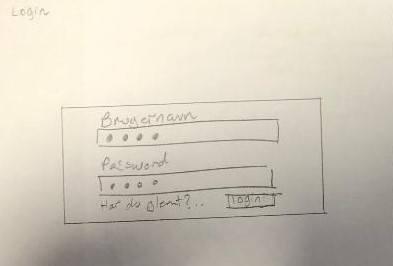
\includegraphics[width=\textwidth]{billeder/login-view.jpg}
			\caption{Login interface}
			\label{fig:1-Login}
		\end{subfigure}
		\quad
		\begin{subfigure}[b]{0.48\textwidth}
			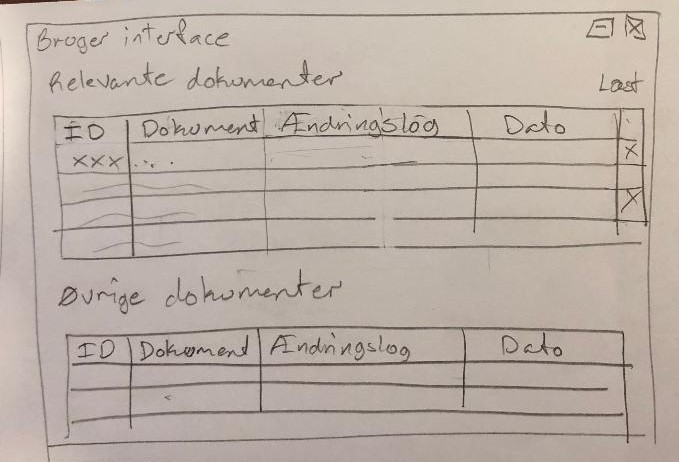
\includegraphics[width=\textwidth]{billeder/Main-view.jpg}
			\caption{Main page interface}
			\label{fig:1-Main}
		\end{subfigure}
\end{figure}
\begin{figure}[H]\ContinuedFloat
		\centering
		\begin{subfigure}[b]{0.48\textwidth}
			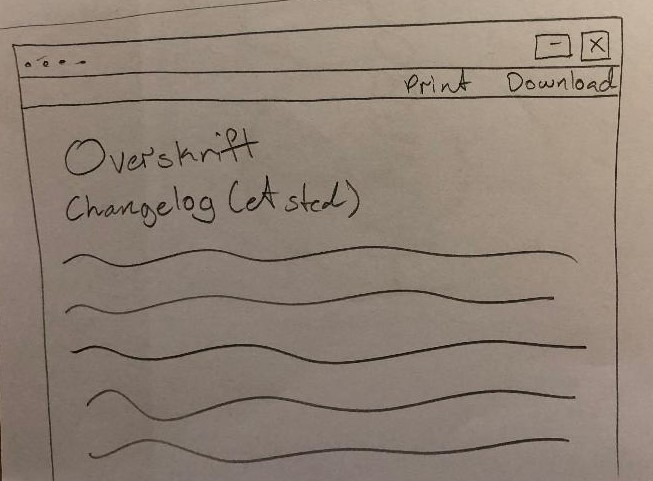
\includegraphics[width=\textwidth]{billeder/pdf-view.jpg}
			\caption{Pdf interface}
			\label{fig:1-pdf}
		\end{subfigure}
		\quad
		\begin{subfigure}[b]{0.48\textwidth}
			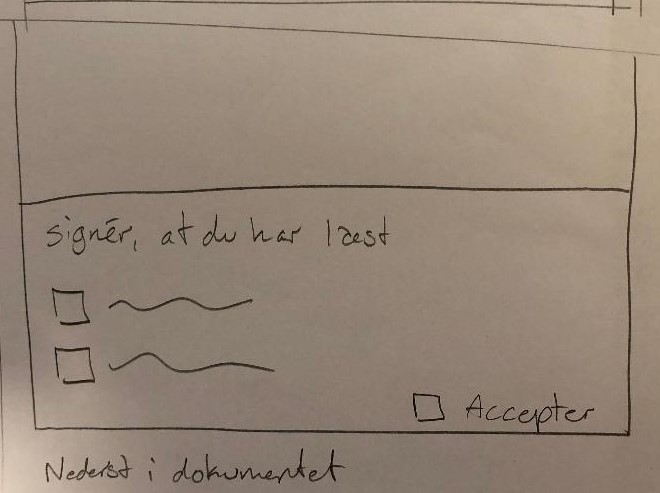
\includegraphics[width=\textwidth]{billeder/bottom-pdf-view.jpg}
			\caption{bottom of pdf view}
			\label{fig:1-bottom-pdf}
		\end{subfigure}
		\caption{Main interfaces and its connections}\label{fig:1-MainPages}
\end{figure}

%Second block of pictures
\begin{figure}[H]
	\centering
		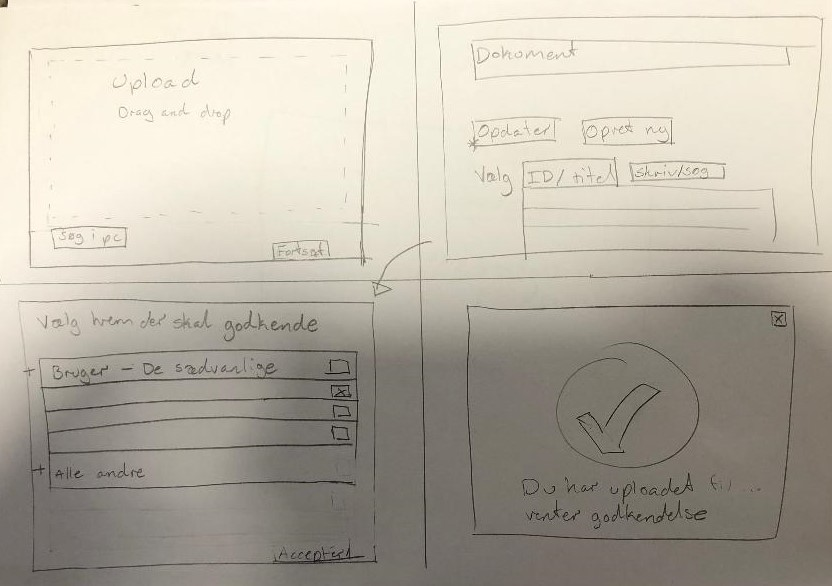
\includegraphics[width=0.65\textwidth]{billeder/Upload-view.jpg}
		\caption{The different interfaces during the upload process}
		\label{fig:1-Upload}
\end{figure}

%Third block of pictures
\begin{figure}[H]
	\centering
	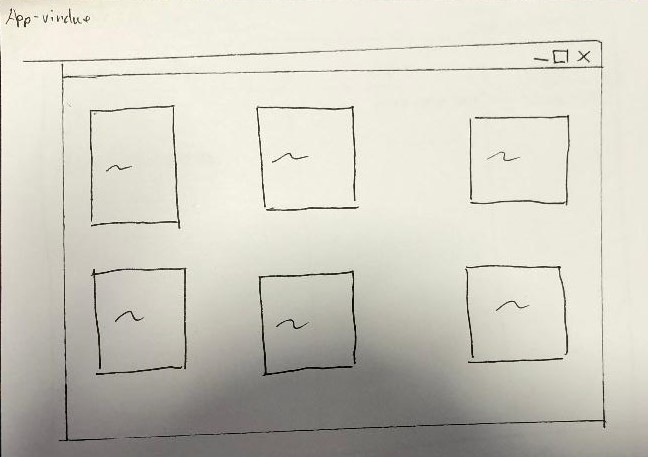
\includegraphics[width=0.5\textwidth]{billeder/app-view.jpg}
	\caption{Interface for first page after login}
	\label{fig:1-app-view}
\end{figure}

\section{Second sketches}\label{sec:Second-sketches}
\begin{figure}[H]
	\centering
	\begin{subfigure}[b]{0.48\textwidth}
		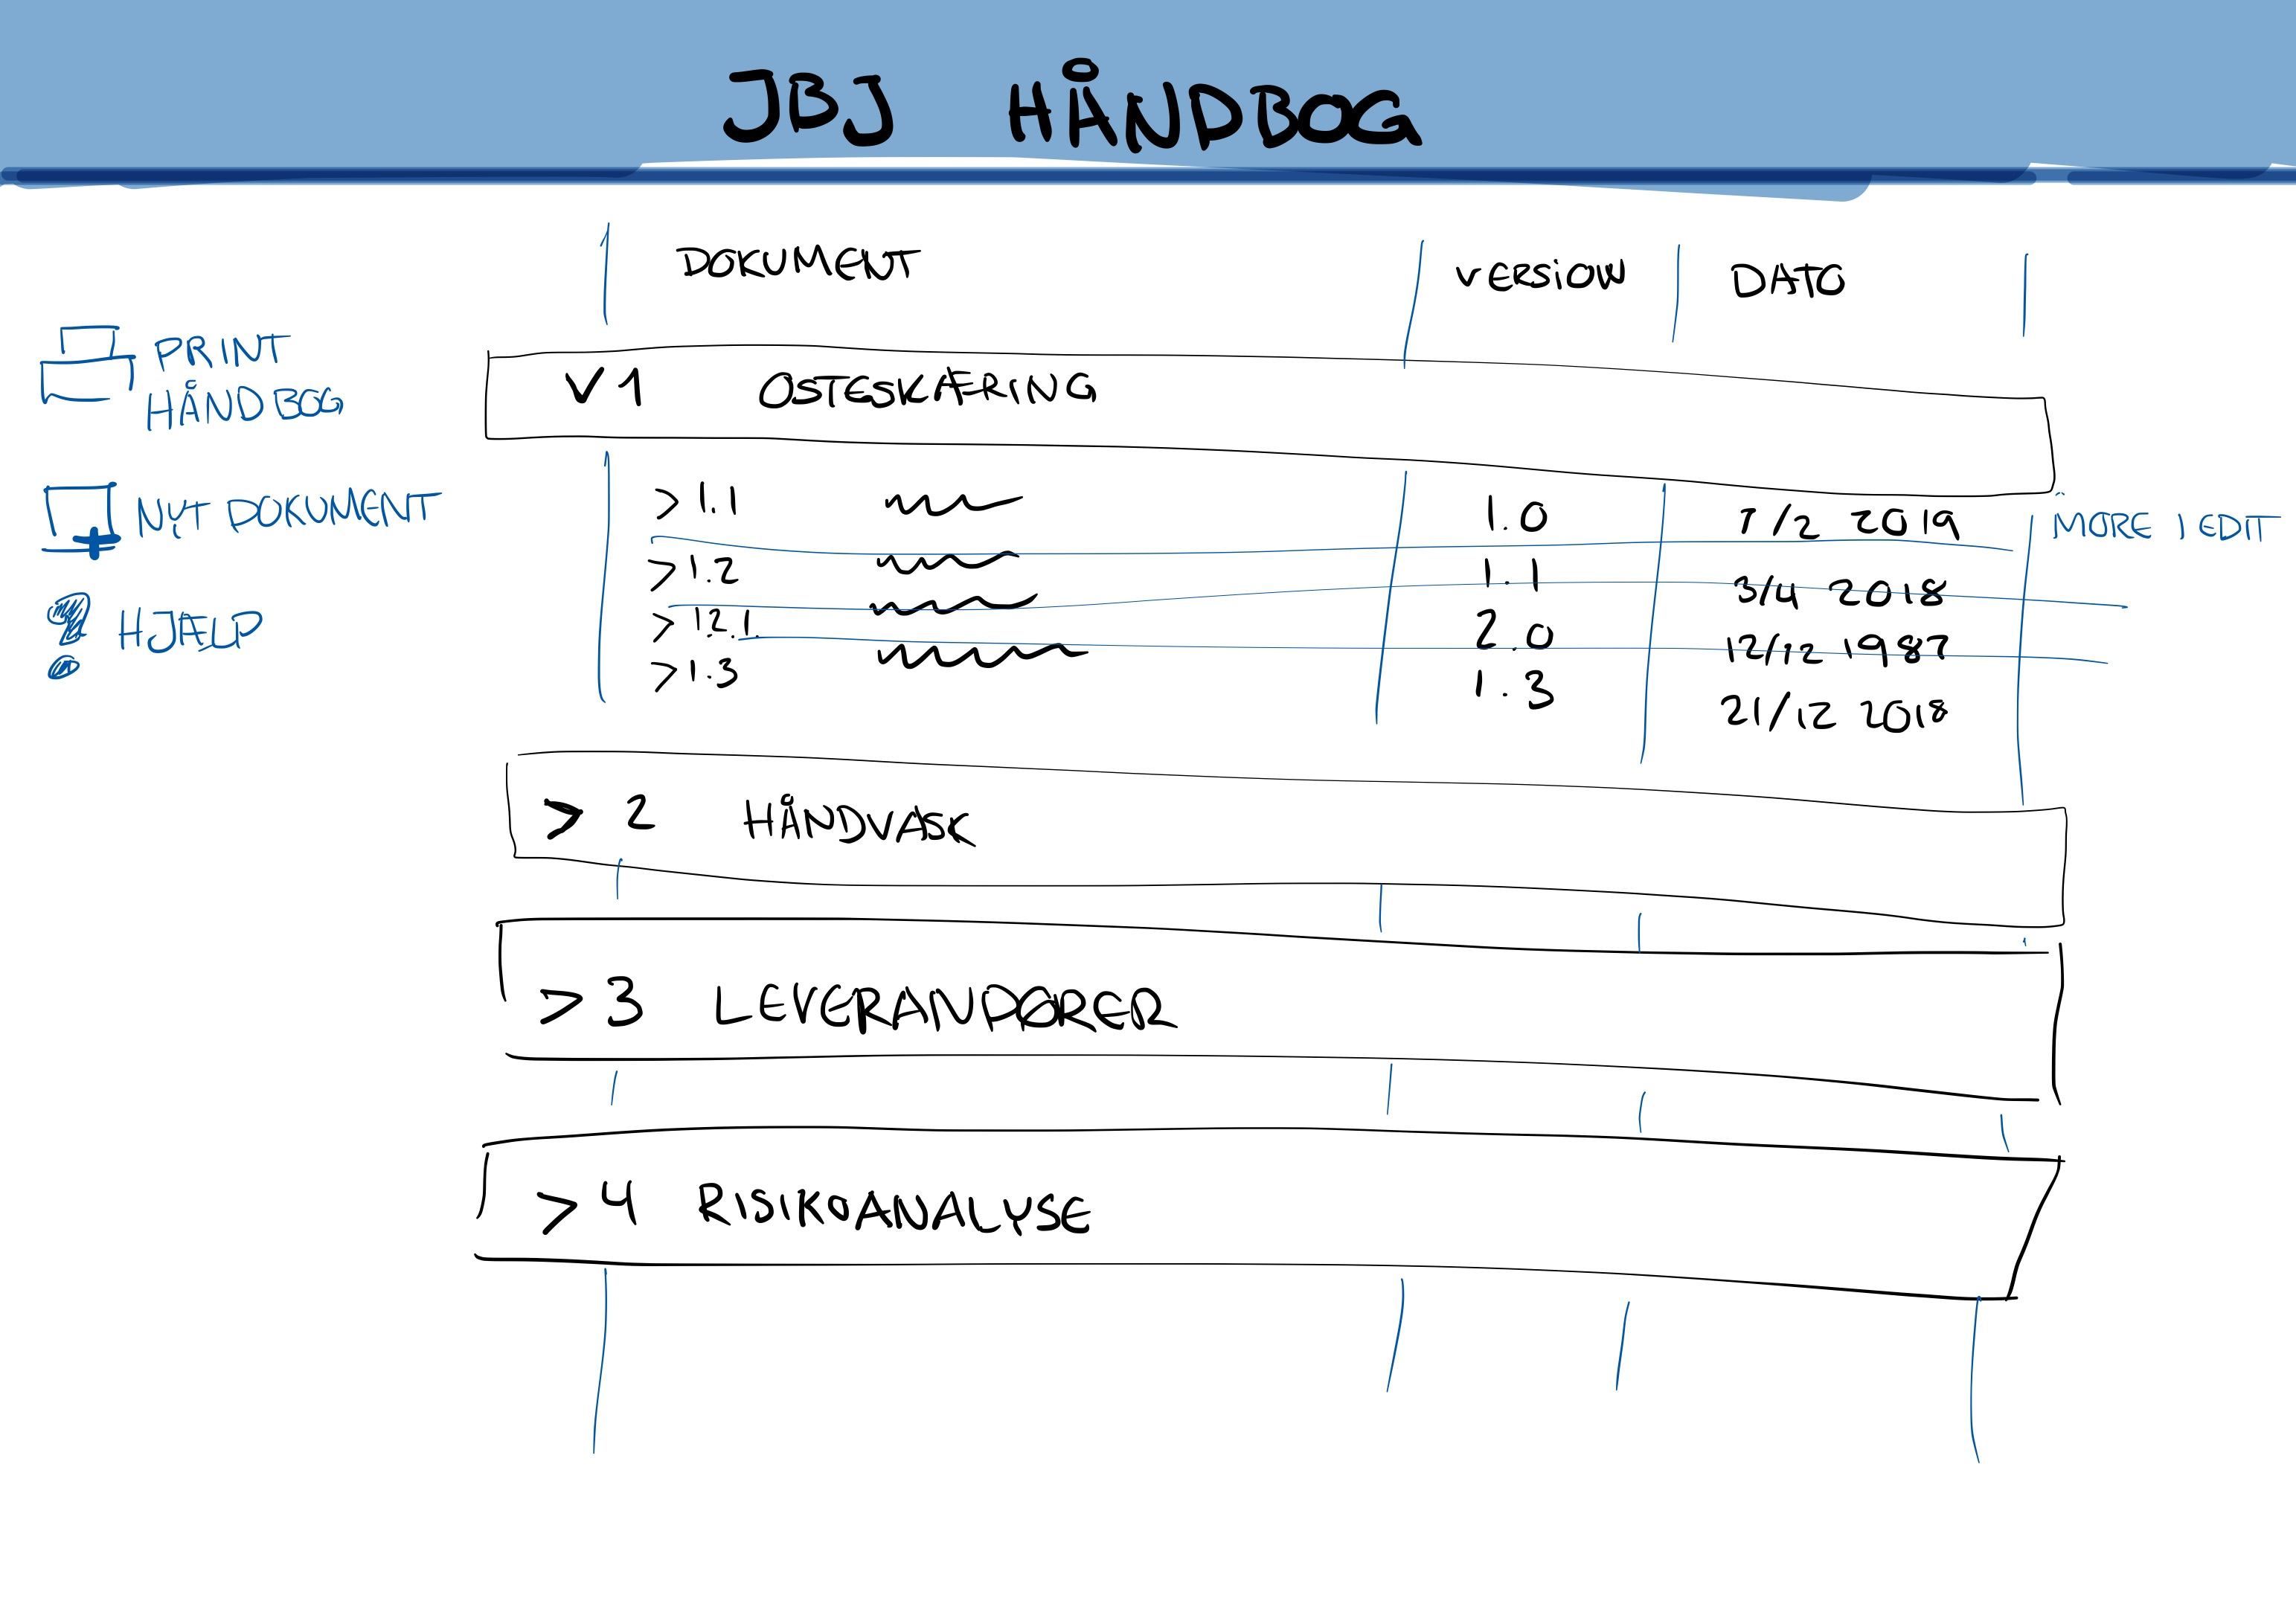
\includegraphics[width=\textwidth]{billeder/Main-view2.jpg}
		\caption{Main page interface}
		\label{fig:2-Main}
	\end{subfigure}
	\quad
	\begin{subfigure}[b]{0.48\textwidth}
		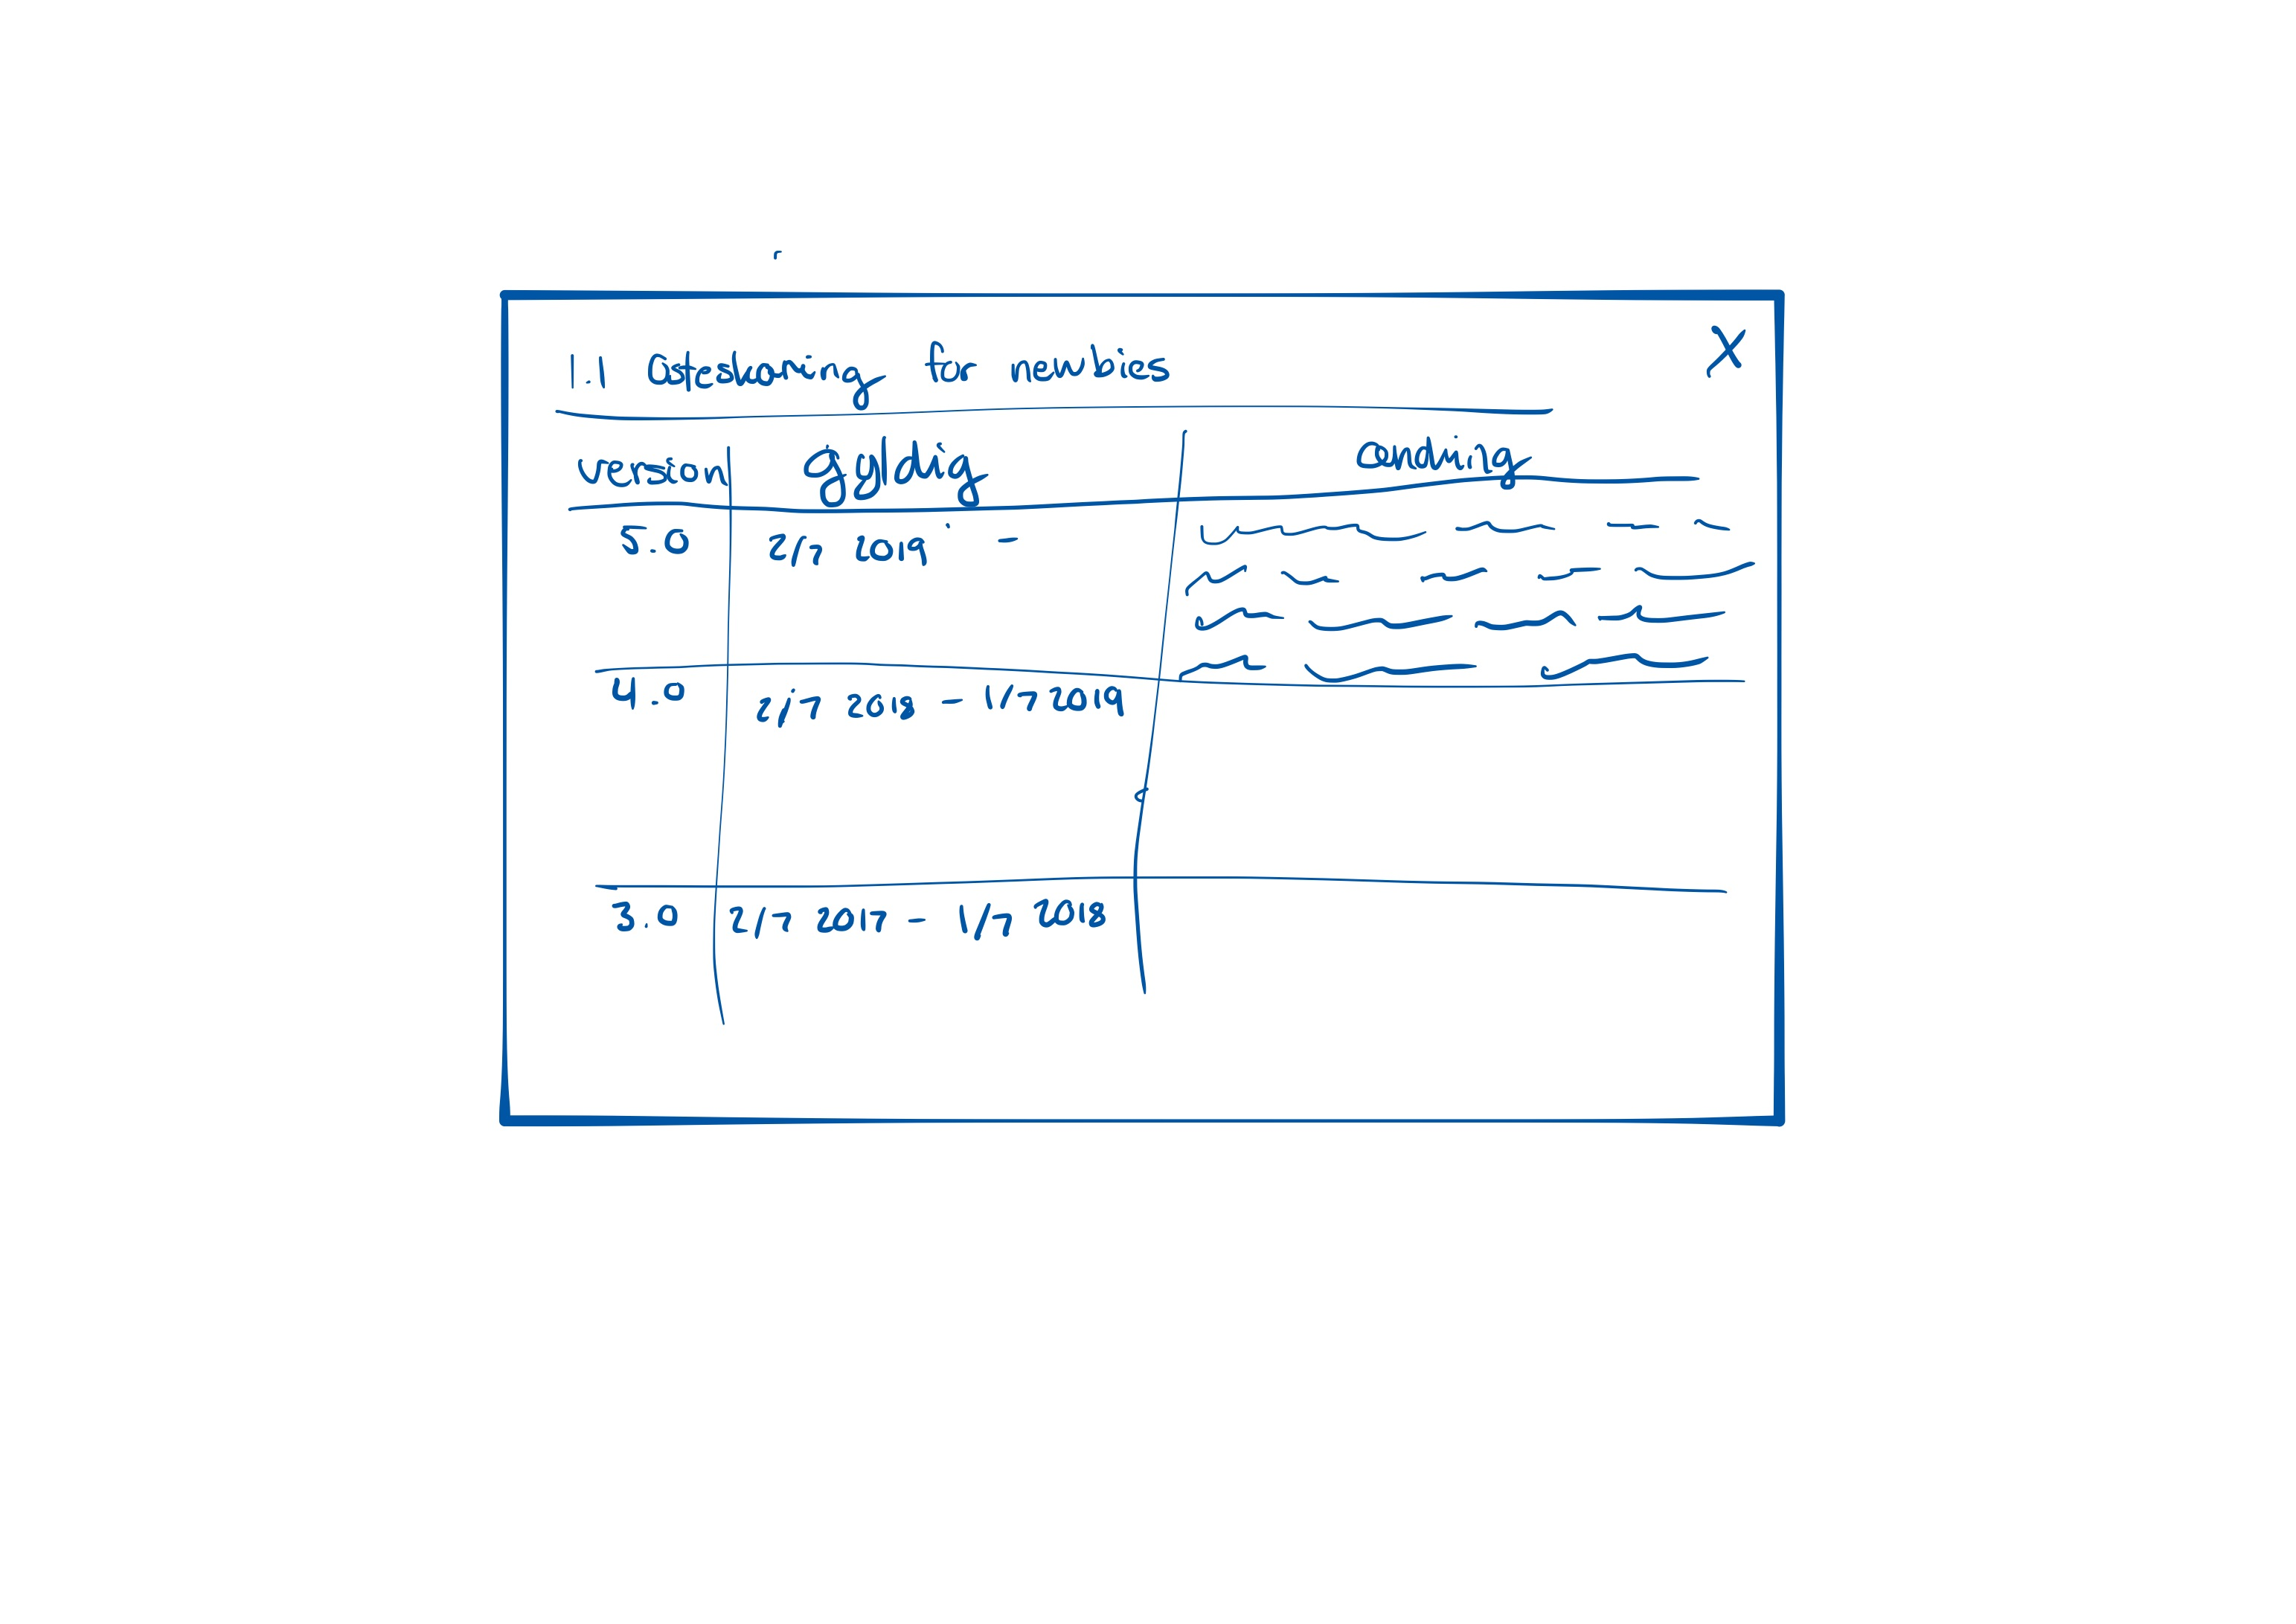
\includegraphics[width=\textwidth]{billeder/Archive-view2.jpg}
		\caption{Archive view of one document}
		\label{fig:2-Archive}
	\end{subfigure}
	\caption{Another idea of how to make the main interface and archive look as well as the archive for one document}
\end{figure}

\newpage
\section{Main interfaces from prototype for second meeting with Ipsen}\label{sec:1prototype}
%Første gruppering af billeder
\begin{figure}[H]
	\centering
	\begin{subfigure}[b]{0.48\textwidth}
		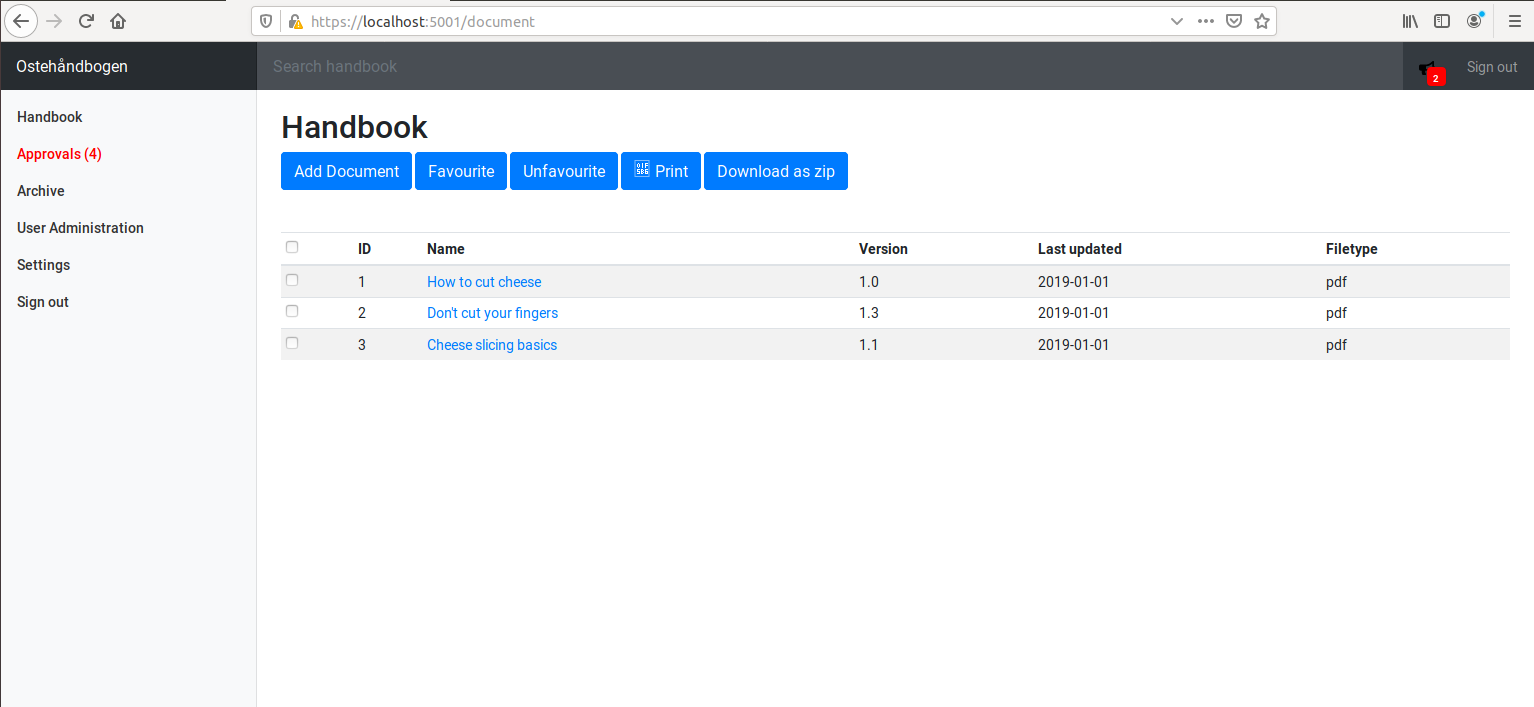
\includegraphics[width=\textwidth]{billeder/iteration1Prototyper/Handbook.png}
		\caption{Main interface}
		\label{fig:3-main}
	\end{subfigure}
	\quad
	\begin{subfigure}[b]{0.48\textwidth}
		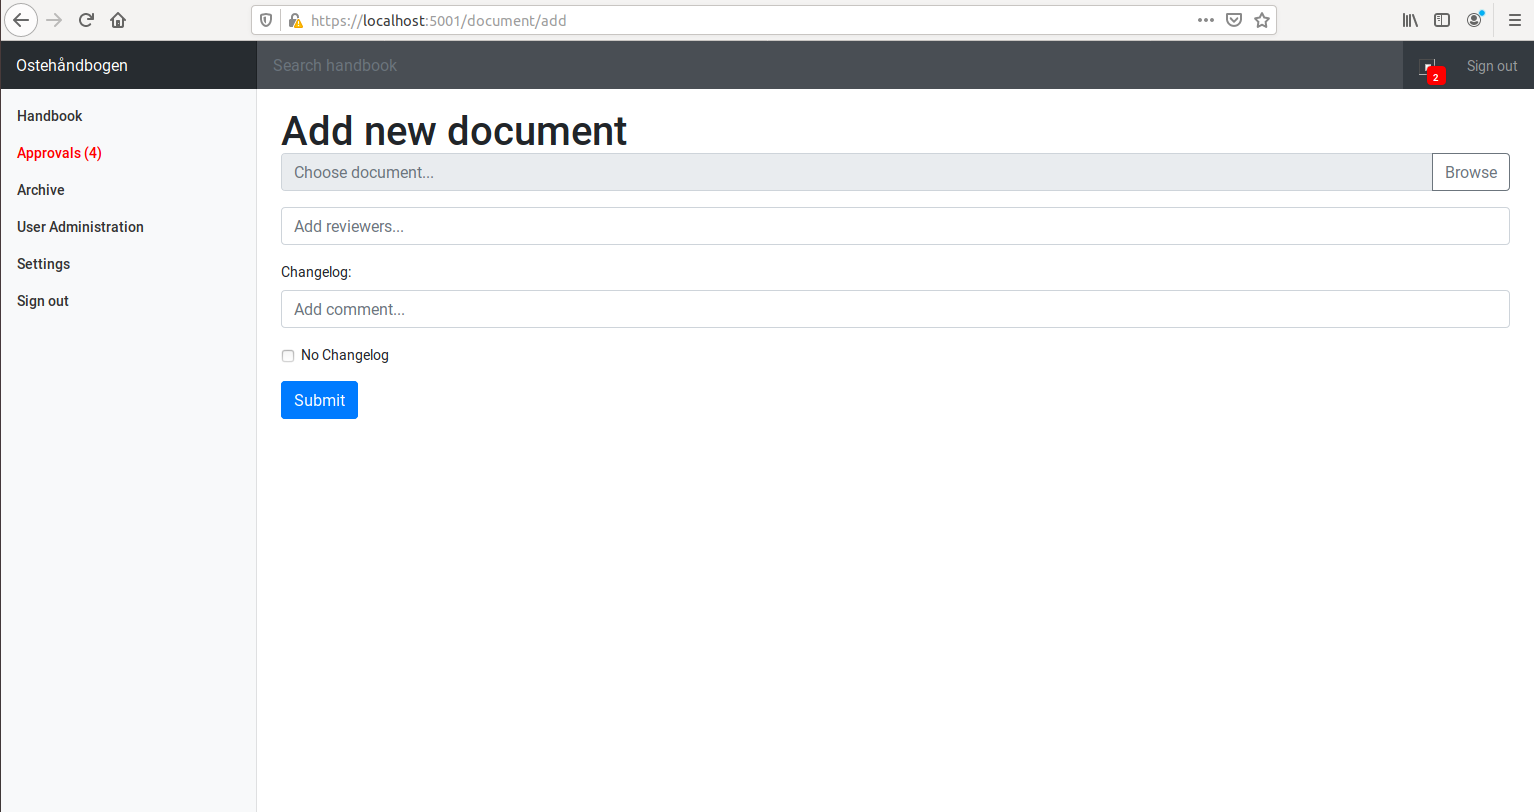
\includegraphics[width=\textwidth]{billeder/iteration1Prototyper/Add-Document.png}
		\caption{View after pressing ''Add Document'' in main interface}
		\label{fig:3-addDoc}
	\end{subfigure}
\end{figure}
\begin{figure}[H]\ContinuedFloat
	\centering
	\begin{subfigure}[b]{0.48\textwidth}
		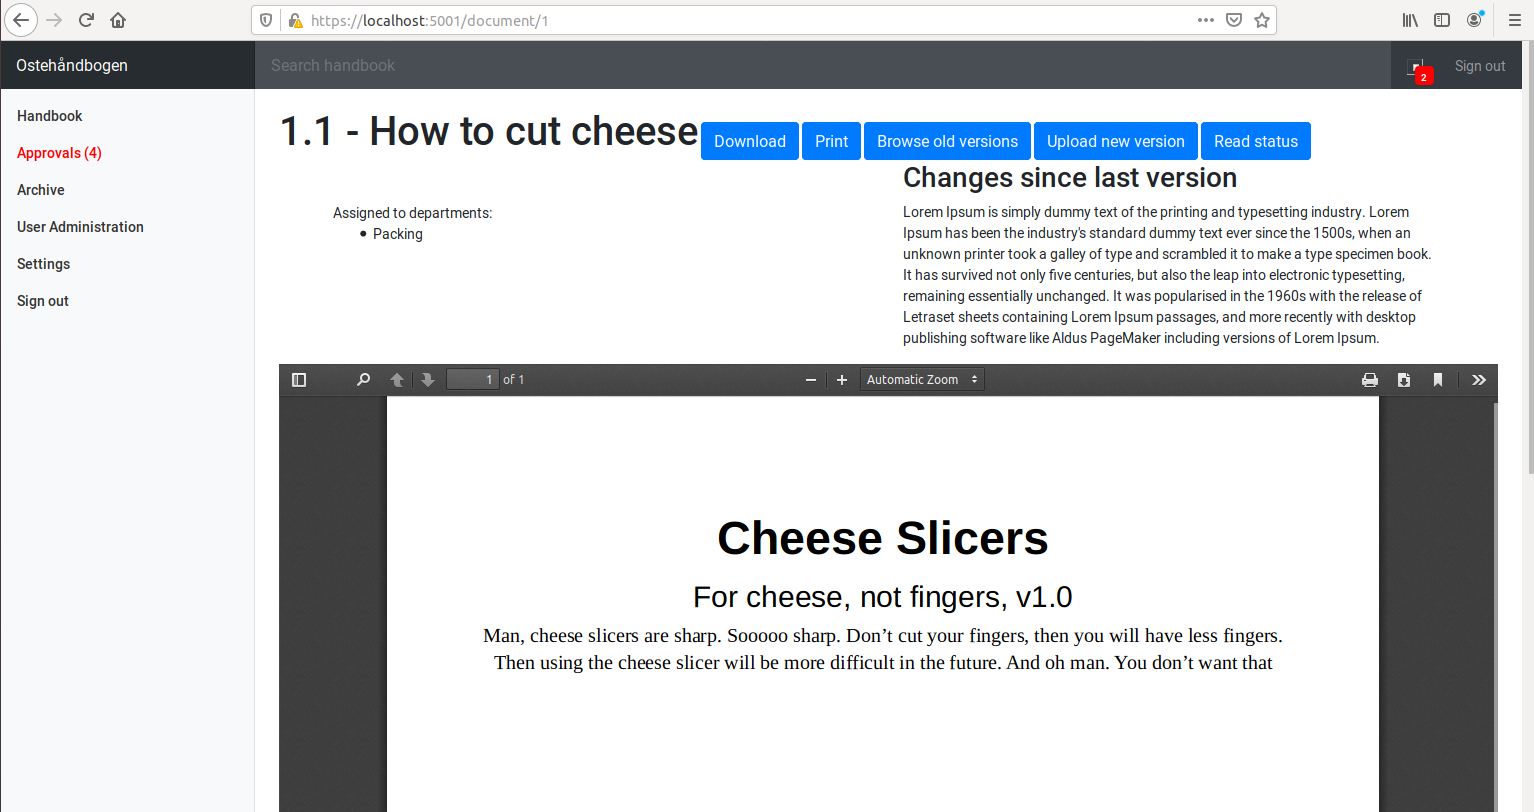
\includegraphics[width=\textwidth]{billeder/iteration1Prototyper/Document-view.png}
		\caption{View of active version in specific Document}
		\label{fig:3-DocView}
	\end{subfigure}
	\quad
	\begin{subfigure}[b]{0.48\textwidth}
		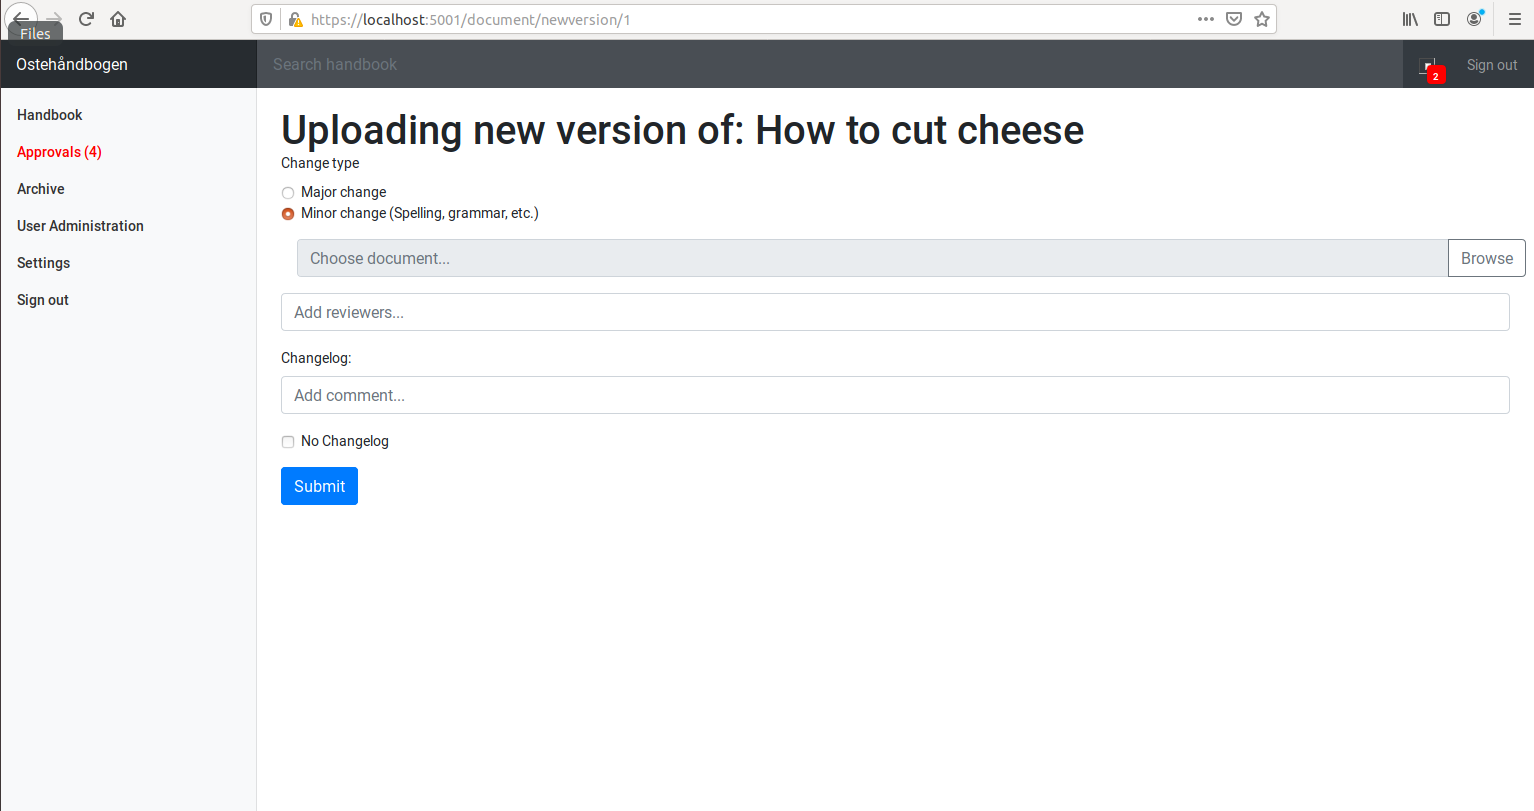
\includegraphics[width=\textwidth]{billeder/iteration1Prototyper/Upload-version.png}
		\caption{View after pressing ''Upload new version''}
		\label{fig:3-UploadVer}
	\end{subfigure}
	\caption{Interfaces connected to main page}\label{fig:3-MainPages}
\end{figure}

%Anden gruppering af billeder
\begin{figure}[H]
	\centering
	\begin{subfigure}[b]{0.48\textwidth}
		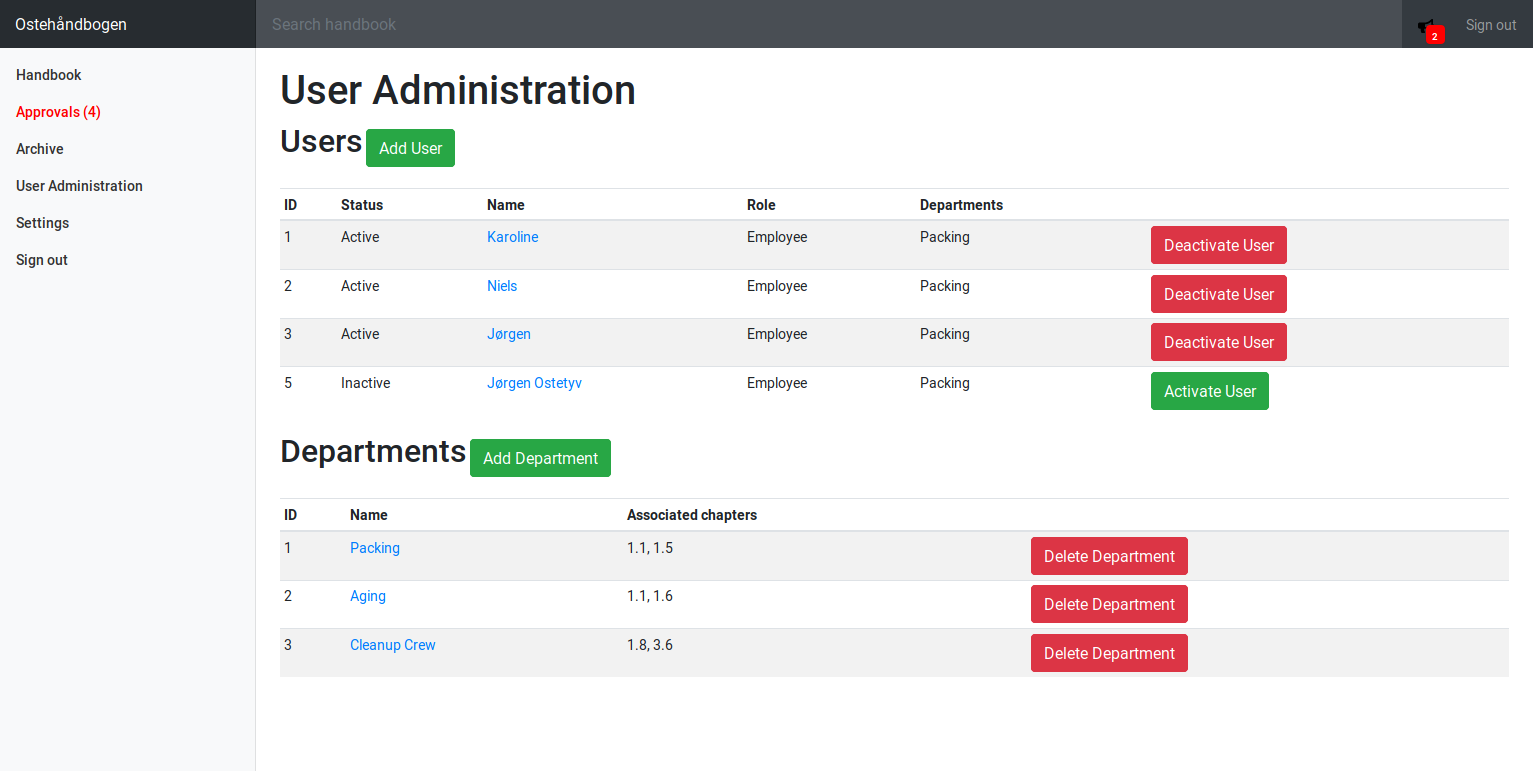
\includegraphics[width=\textwidth]{billeder/iteration1Prototyper/UserAdministration.png}
		\caption{User administration interface}
		\label{fig:3-UserAdmin}
	\end{subfigure}
	\quad
	\begin{subfigure}[b]{0.48\textwidth}
		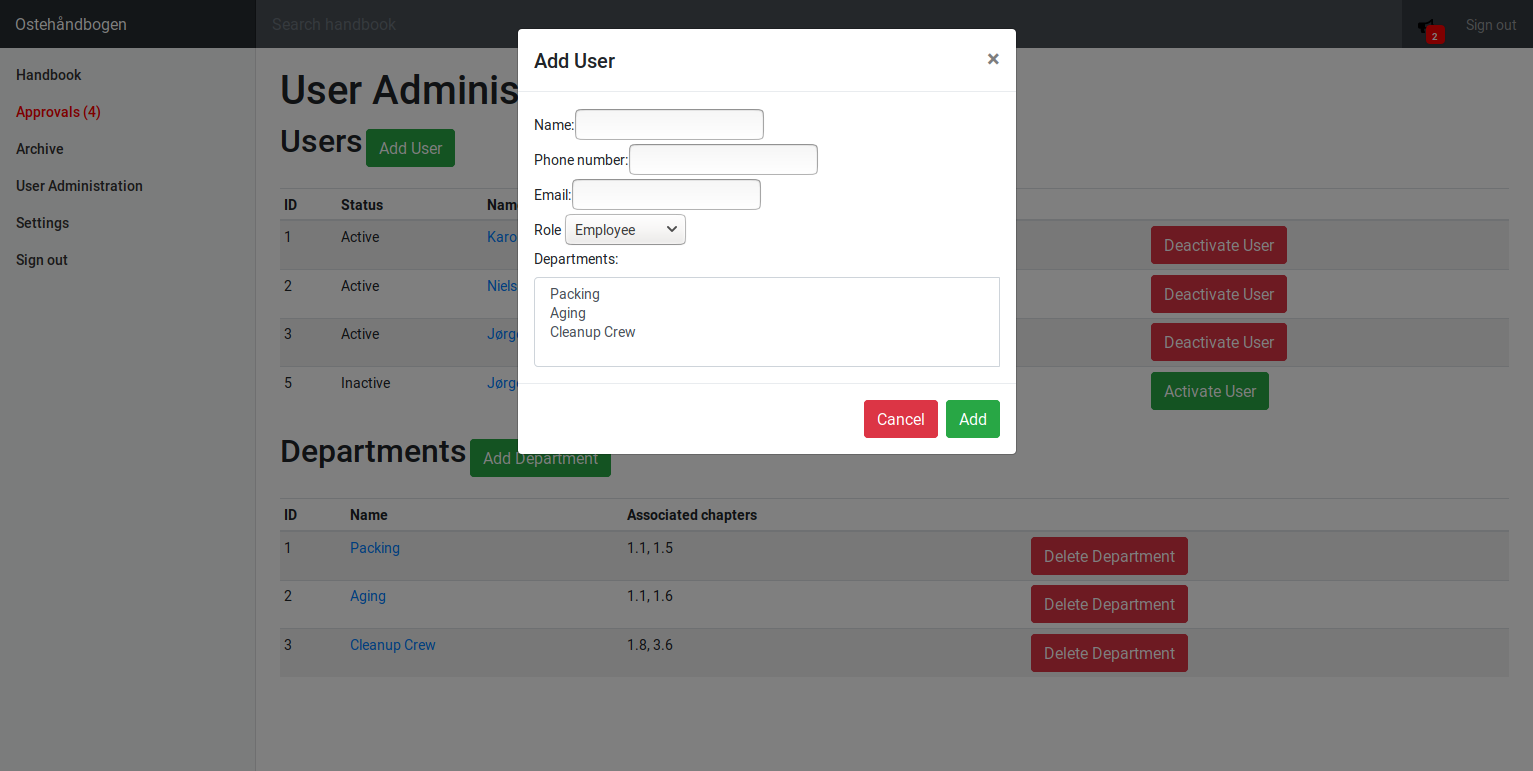
\includegraphics[width=\textwidth]{billeder/iteration1Prototyper/AddUser.png}
		\caption{Add new user view}
		\label{fig:3-addUser}
	\end{subfigure}
\end{figure}
\begin{figure}[H]\ContinuedFloat
	\centering
	\begin{subfigure}[b]{0.48\textwidth}
		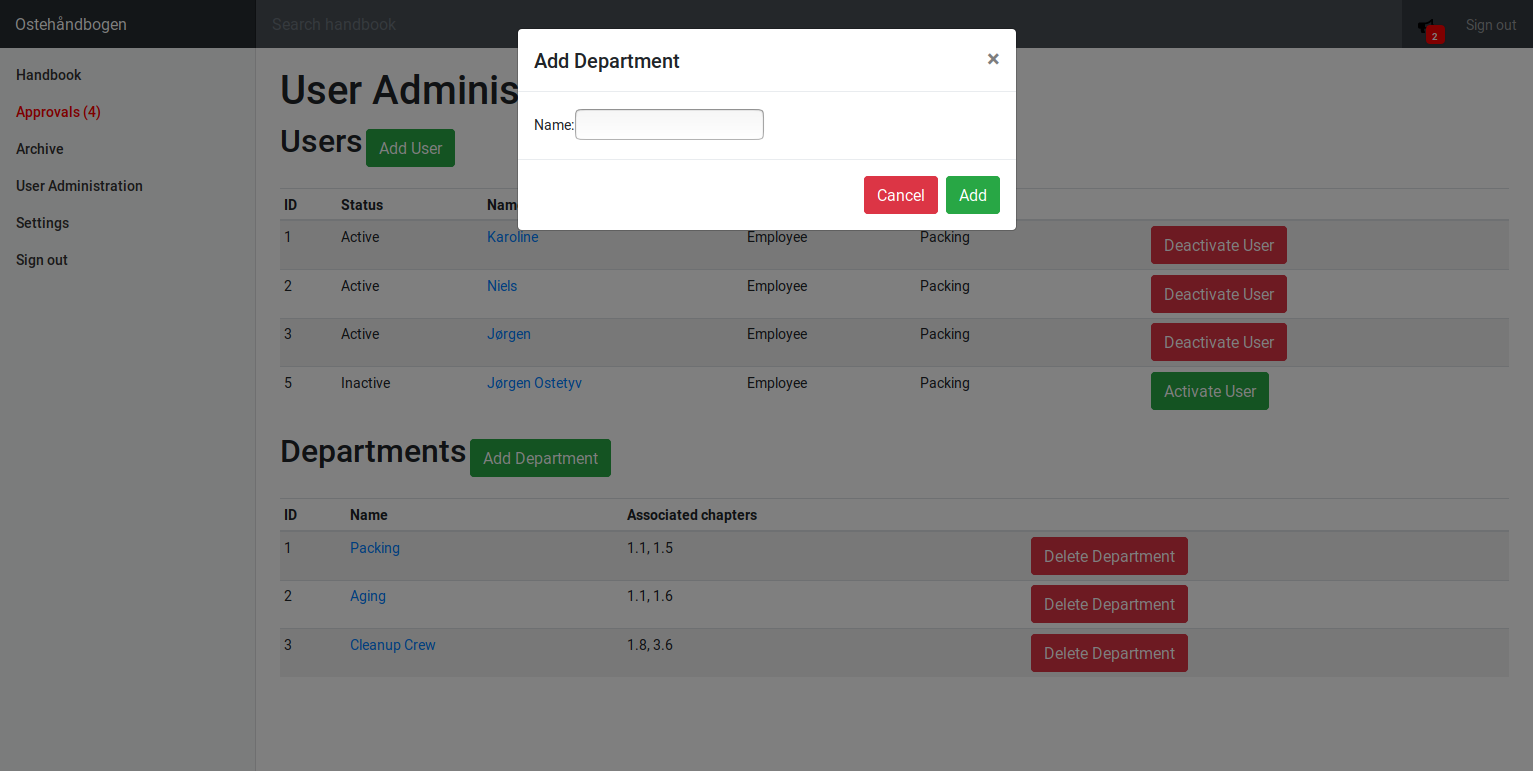
\includegraphics[width=\textwidth]{billeder/iteration1Prototyper/AddDepartment.png}
		\caption{Add new department}
		\label{fig:3-AddDep}
	\end{subfigure}
	\quad
	\begin{subfigure}[b]{0.48\textwidth}
		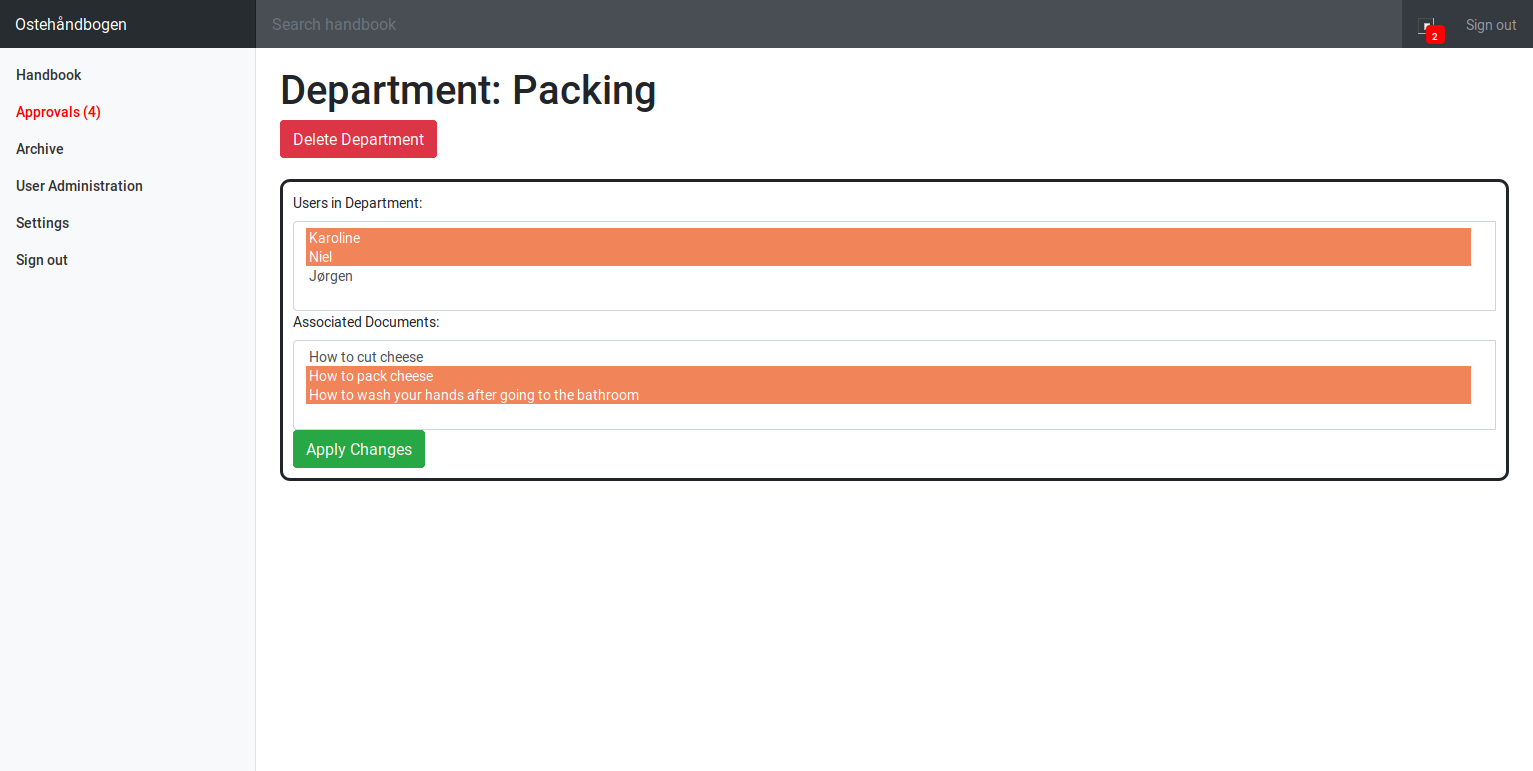
\includegraphics[width=\textwidth]{billeder/iteration1Prototyper/DepartmentEdit.png}
		\caption{Edit existing department}
		\label{fig:3-EditDep}
	\end{subfigure}
	\caption{Interfaces connected user administration}\label{fig:3-UserAdminPages}
\end{figure}

%Tredje gruppering af billeder
\begin{figure}[H]
	\centering
	\begin{subfigure}[b]{0.48\textwidth}
		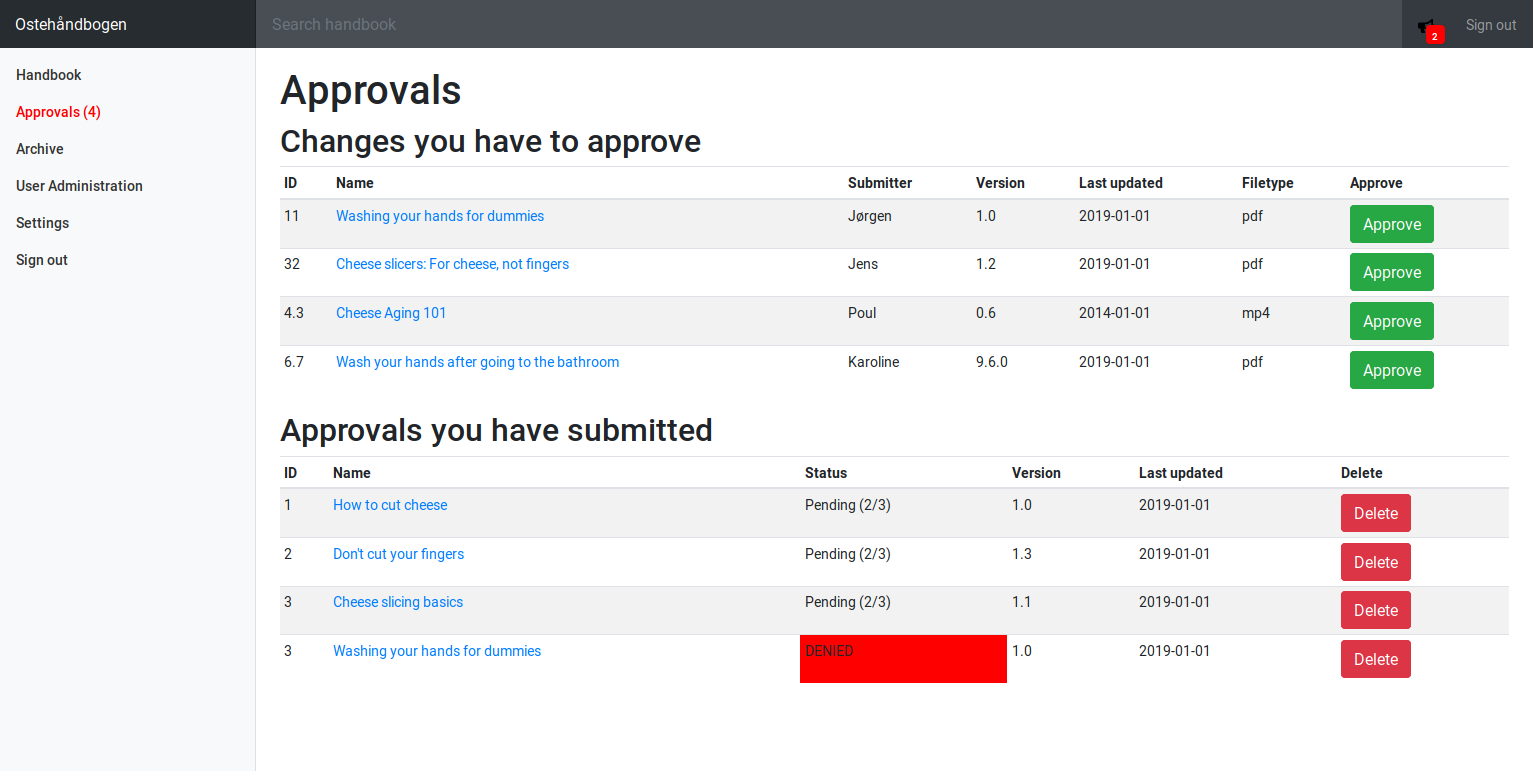
\includegraphics[width=\textwidth]{billeder/iteration1Prototyper/Approval.png}
		\caption{Approval interface}
		\label{fig:3-approve}
	\end{subfigure}
	\quad
	\begin{subfigure}[b]{0.48\textwidth}
		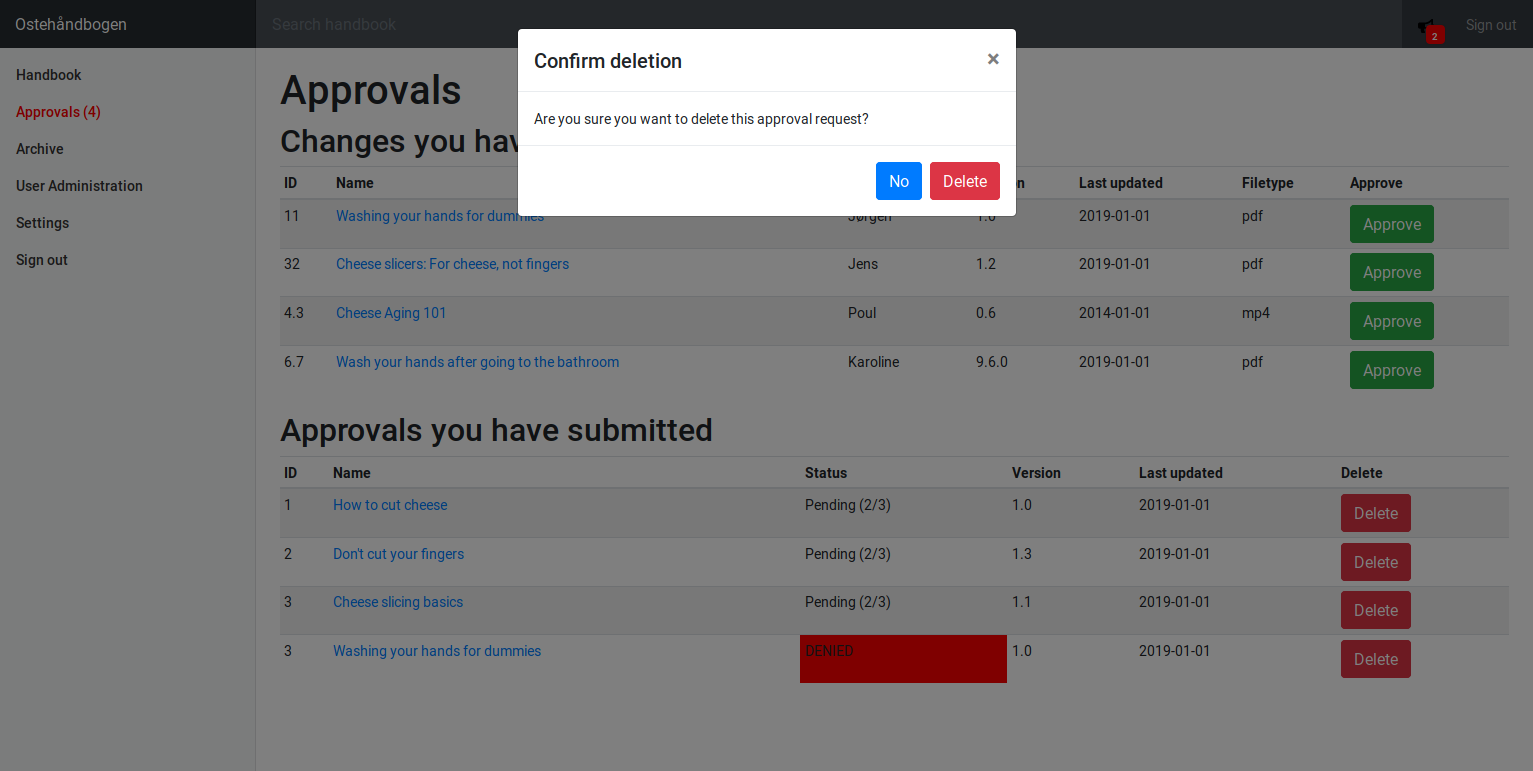
\includegraphics[width=\textwidth]{billeder/iteration1Prototyper/ApprovalDenial.png}
		\caption{Pop up when denying approval.}
		\label{fig:3-ApproveDenial}
	\end{subfigure}
\end{figure}
\begin{figure}[H]\ContinuedFloat
	\centering
	\begin{subfigure}[b]{0.48\textwidth}
		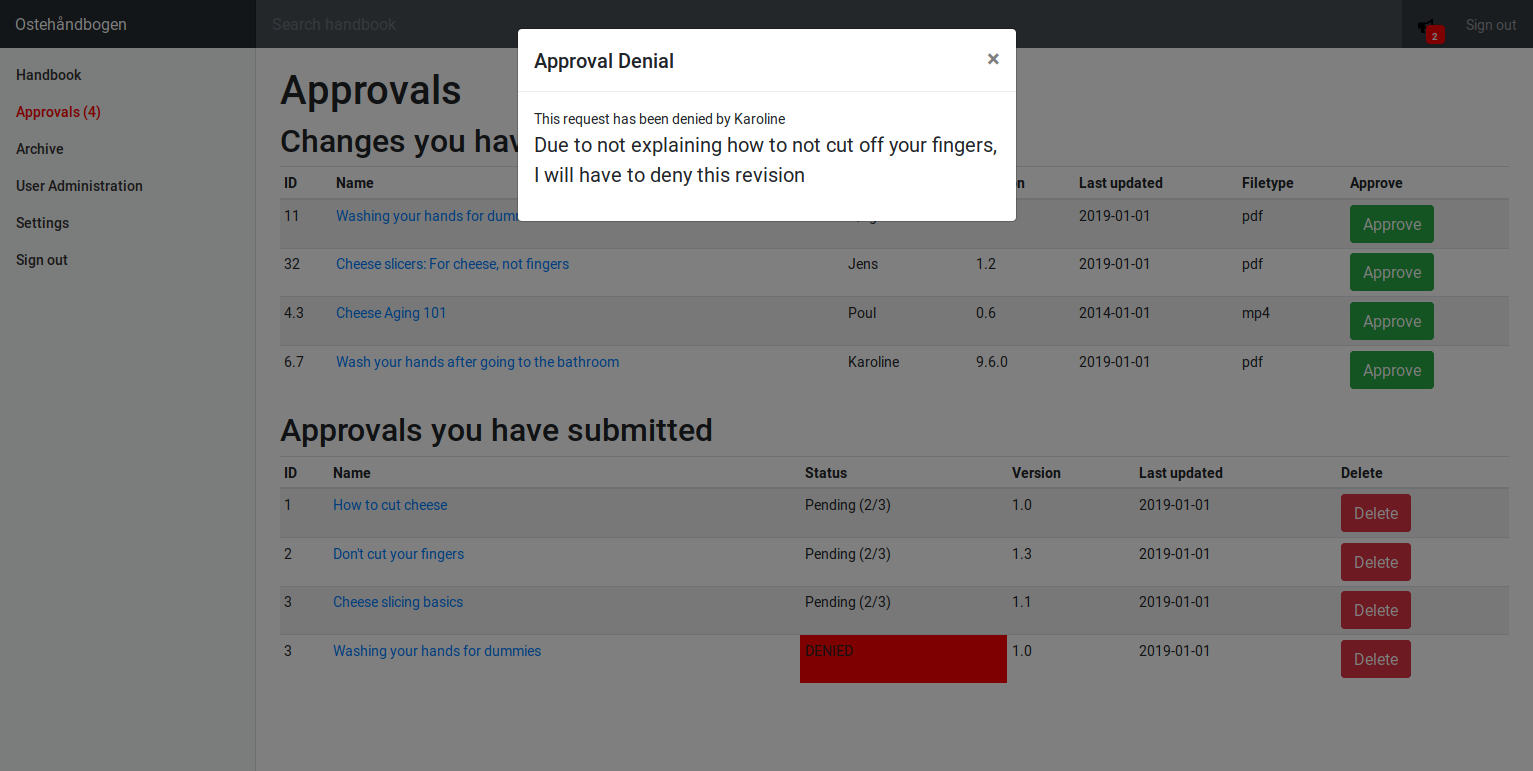
\includegraphics[width=\textwidth]{billeder/iteration1Prototyper/ApprovalDenied.png}
		\caption{when someone else has denied the approval}
		\label{fig:3-ApproveDenied}
	\end{subfigure}
	\quad
	\begin{subfigure}[b]{0.48\textwidth}
		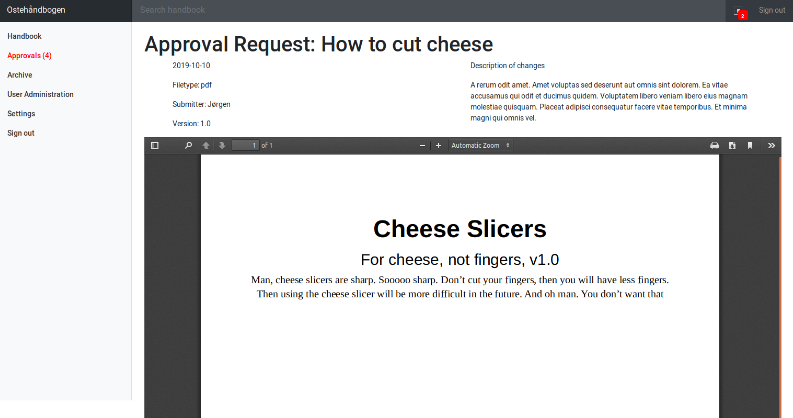
\includegraphics[width=\textwidth]{billeder/iteration1Prototyper/ApprovalRequest.png}
		\caption{Detailed view of an approval request.}
		\label{fig:3-ApproveRequest}
	\end{subfigure}
	\caption{Interfaces connected to Approval process}\label{fig:3-AprovalPages}
\end{figure}

%Fjerde gruppering af billeder
\begin{figure}[H]
	\centering
	\begin{subfigure}[b]{0.48\textwidth}
		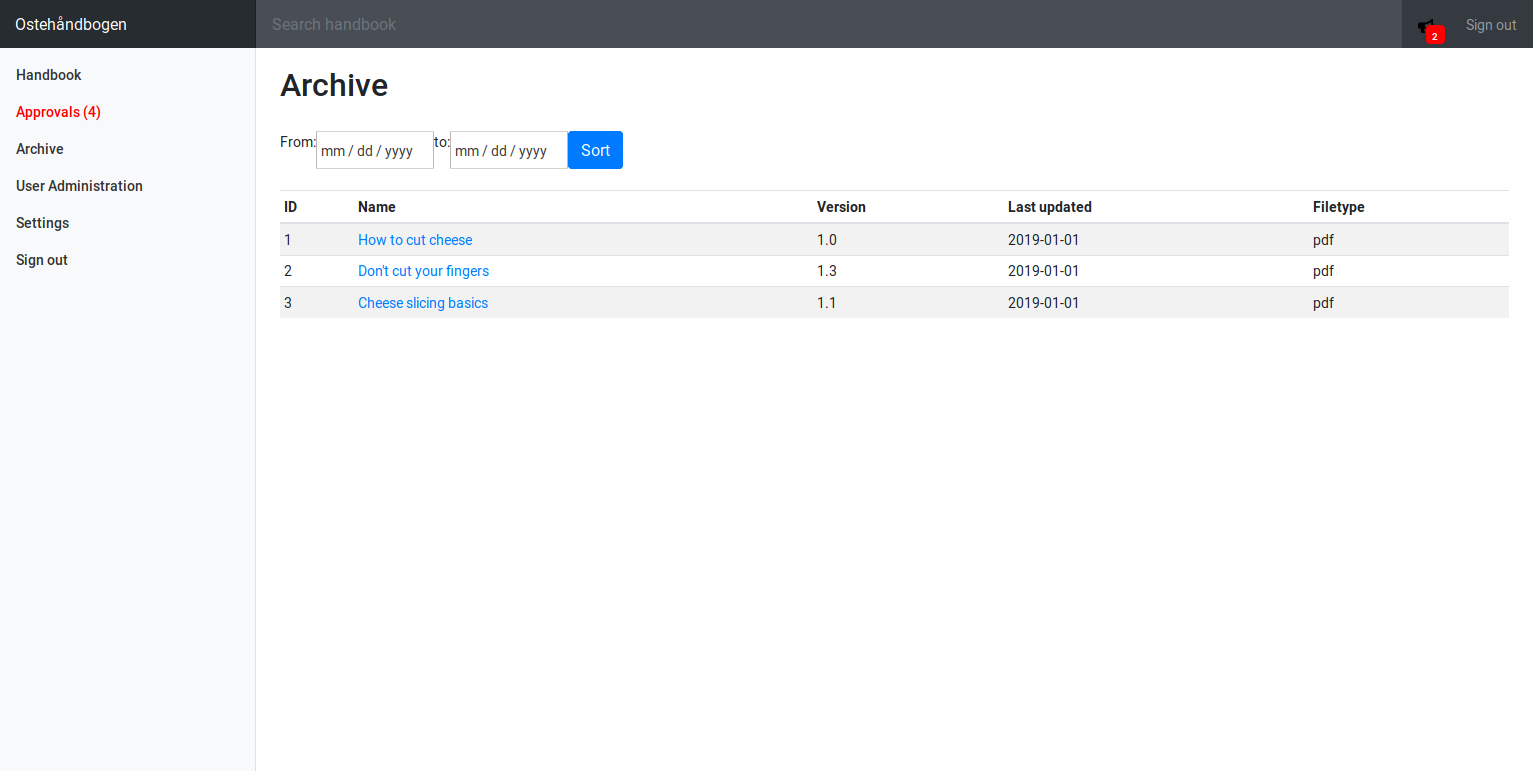
\includegraphics[width=\textwidth]{billeder/iteration1Prototyper/Archive.png}
		\caption{Archive interface}
		\label{fig:3-archive}
	\end{subfigure}
	\quad
	\begin{subfigure}[b]{0.48\textwidth}
		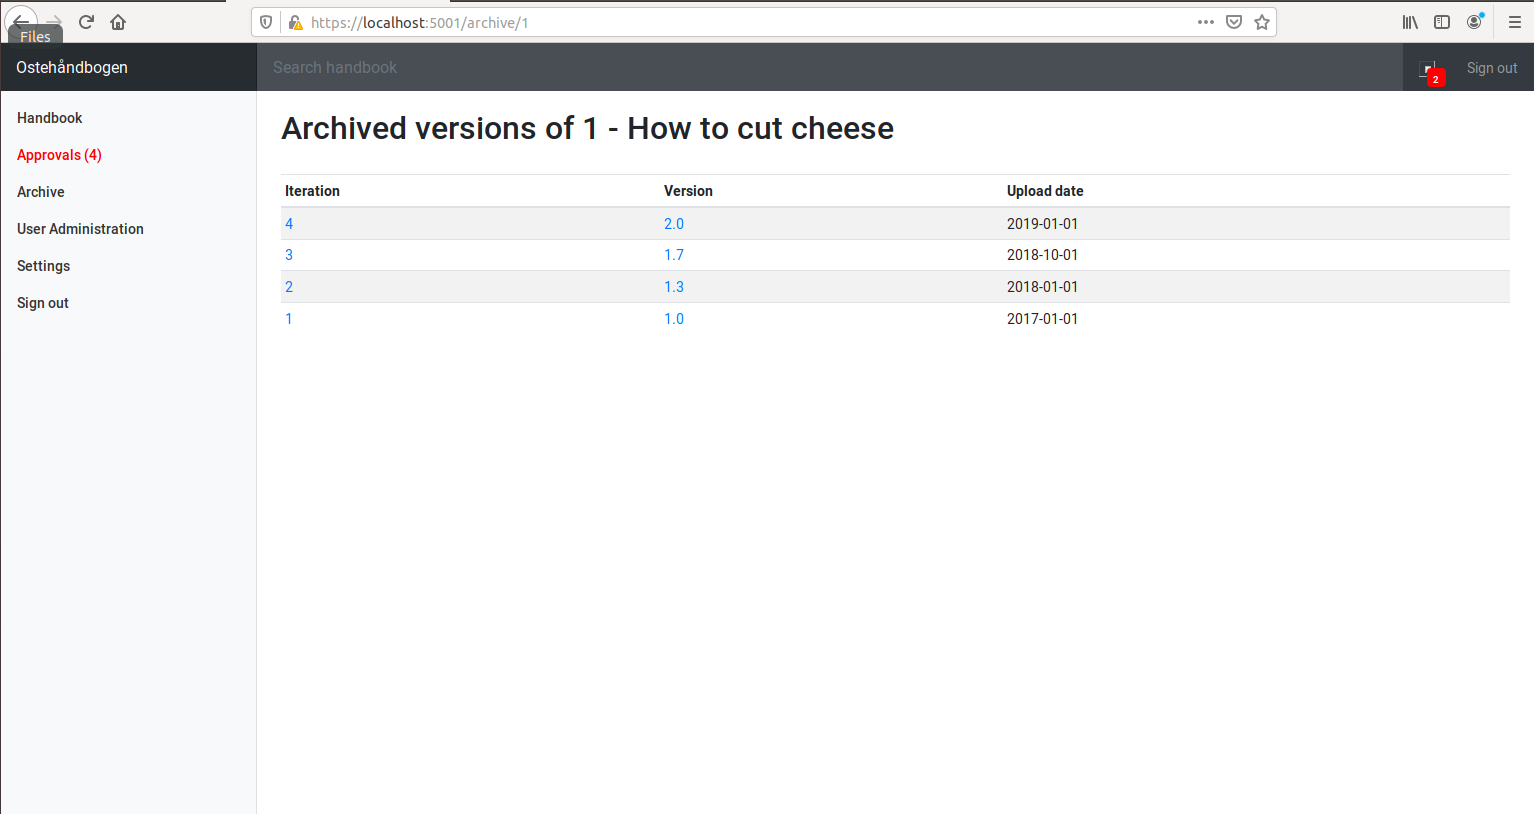
\includegraphics[width=\textwidth]{billeder/iteration1Prototyper/Archive-Version1.png}
		\caption{Archive of a specific document}
		\label{fig:3-ArchiveVersion}
	\end{subfigure}
	\caption{Interfaces connected to the archive}\label{fig:3-ArchivePages}
\end{figure}

\chapter{Second iteration prototypes}\label{chap:2-Prototypes}
\section{Mock-up}\label{sec:Mock}

\begin{figure}[H]
	\centering
	\begin{subfigure}[b]{0.48\textwidth}
		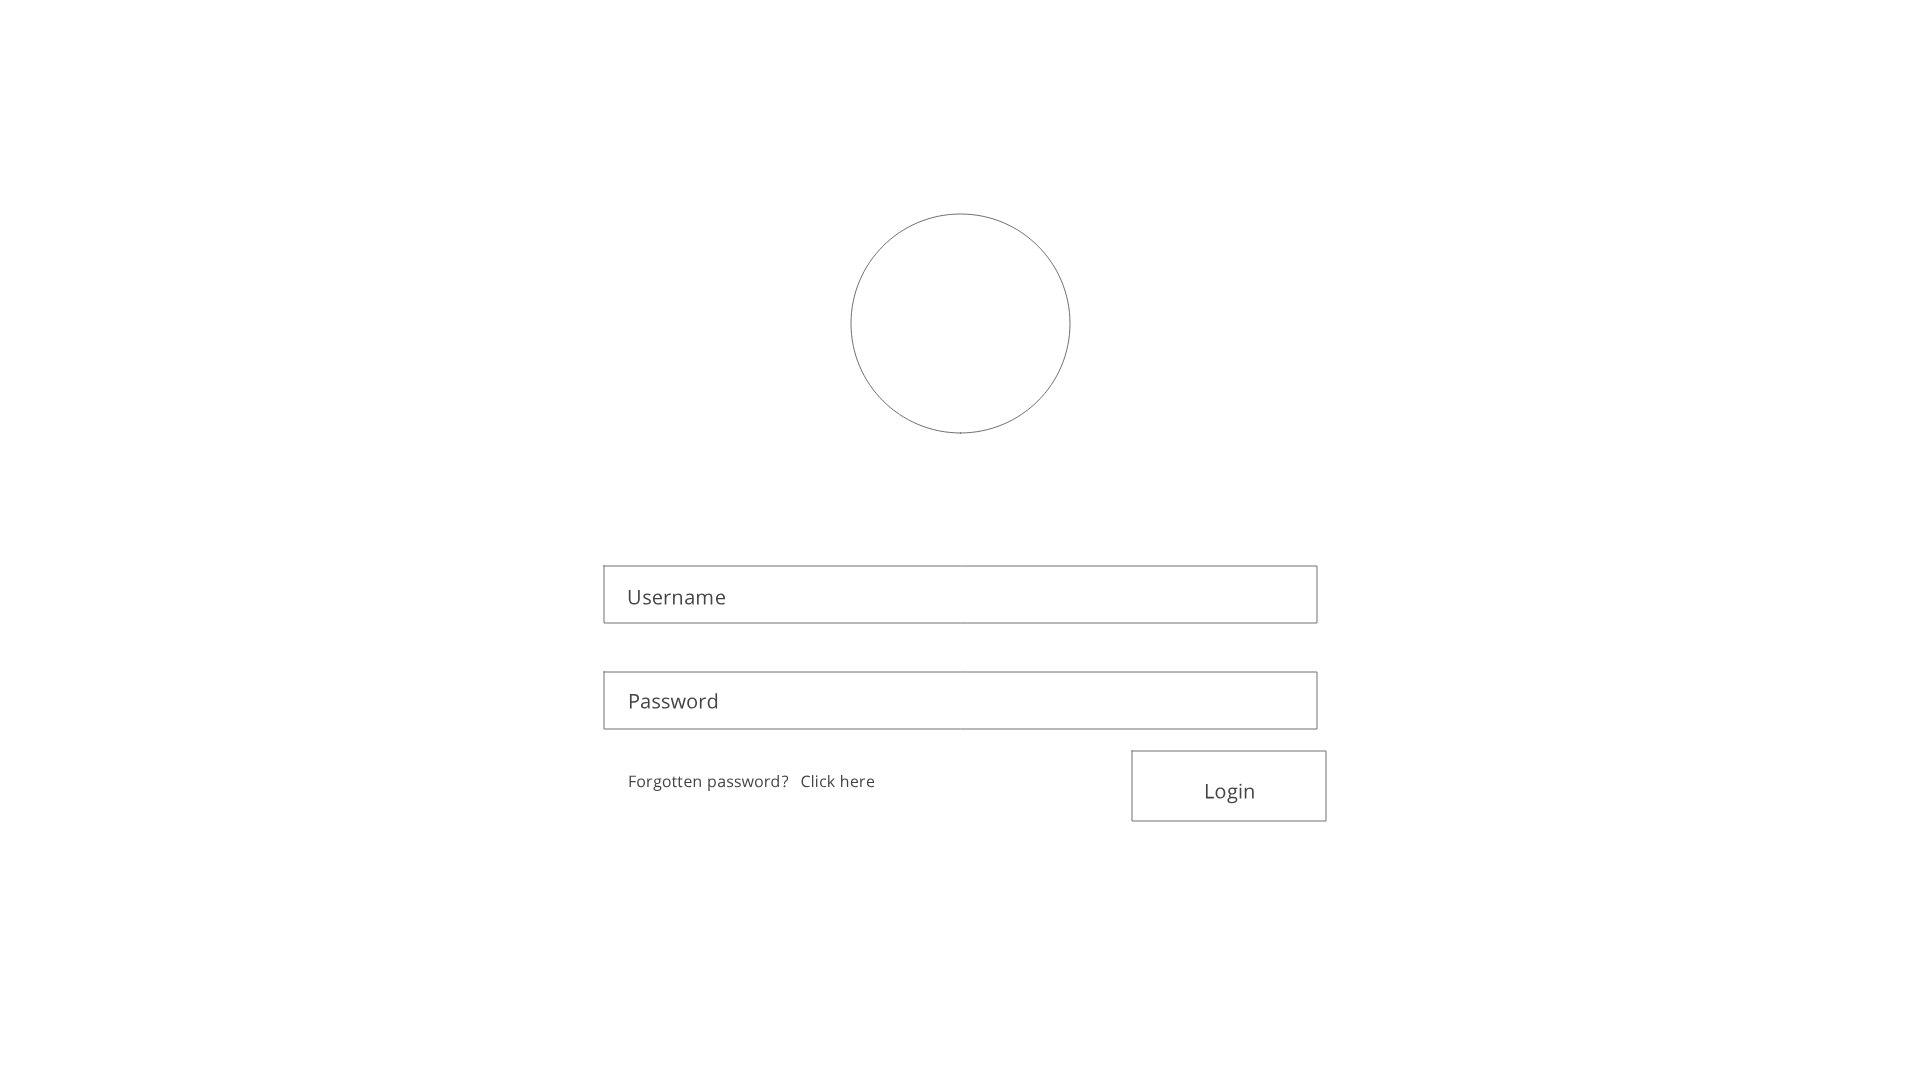
\includegraphics[width=\textwidth]{billeder/iteration2Prototyper/Page_1.jpg}
		\caption{Login interface}
		\label{fig:4-Login}
	\end{subfigure}
	\quad
	\begin{subfigure}[b]{0.48\textwidth}
		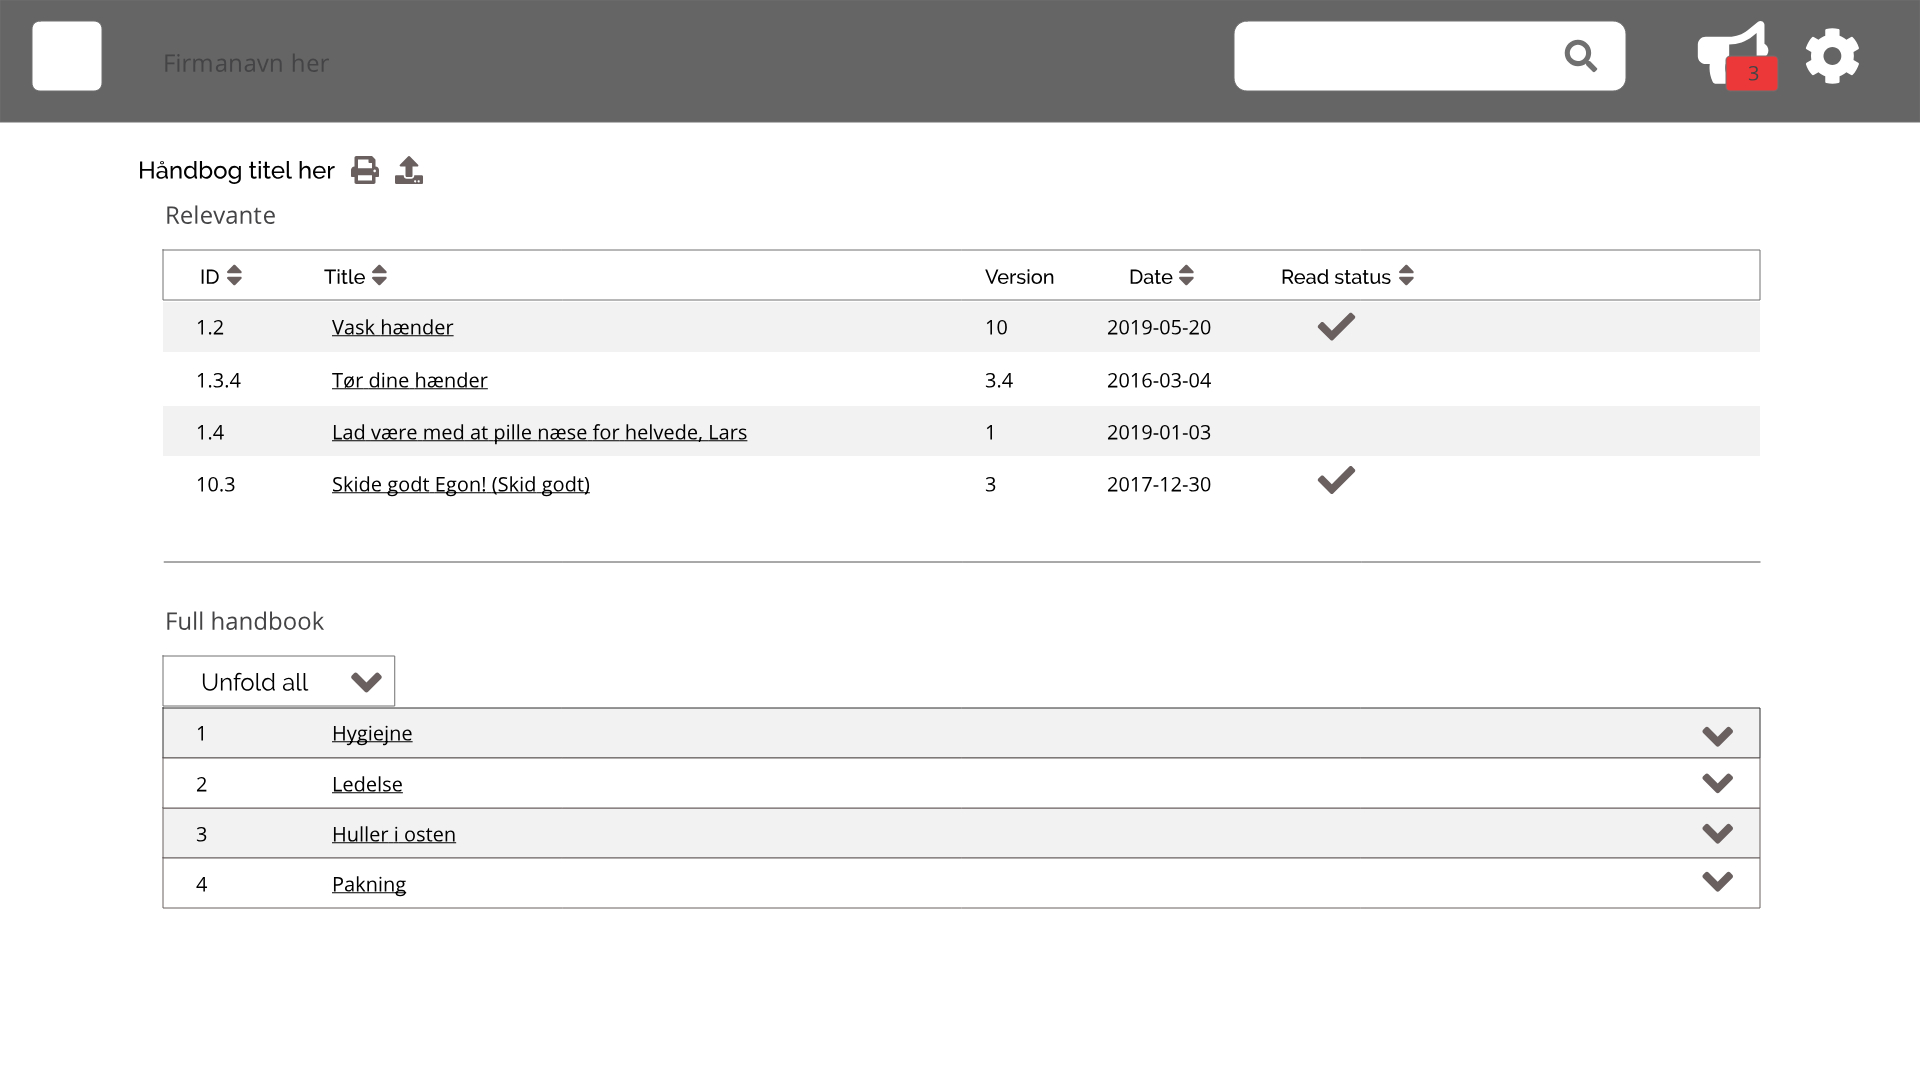
\includegraphics[width=\textwidth]{billeder/iteration2Prototyper/Page_2.jpg}
		\caption{Main page interface for writer}
		\label{fig:4-Main}
	\end{subfigure}
\end{figure}
\begin{figure}[H]\ContinuedFloat
	\centering
	\begin{subfigure}[b]{0.48\textwidth}
		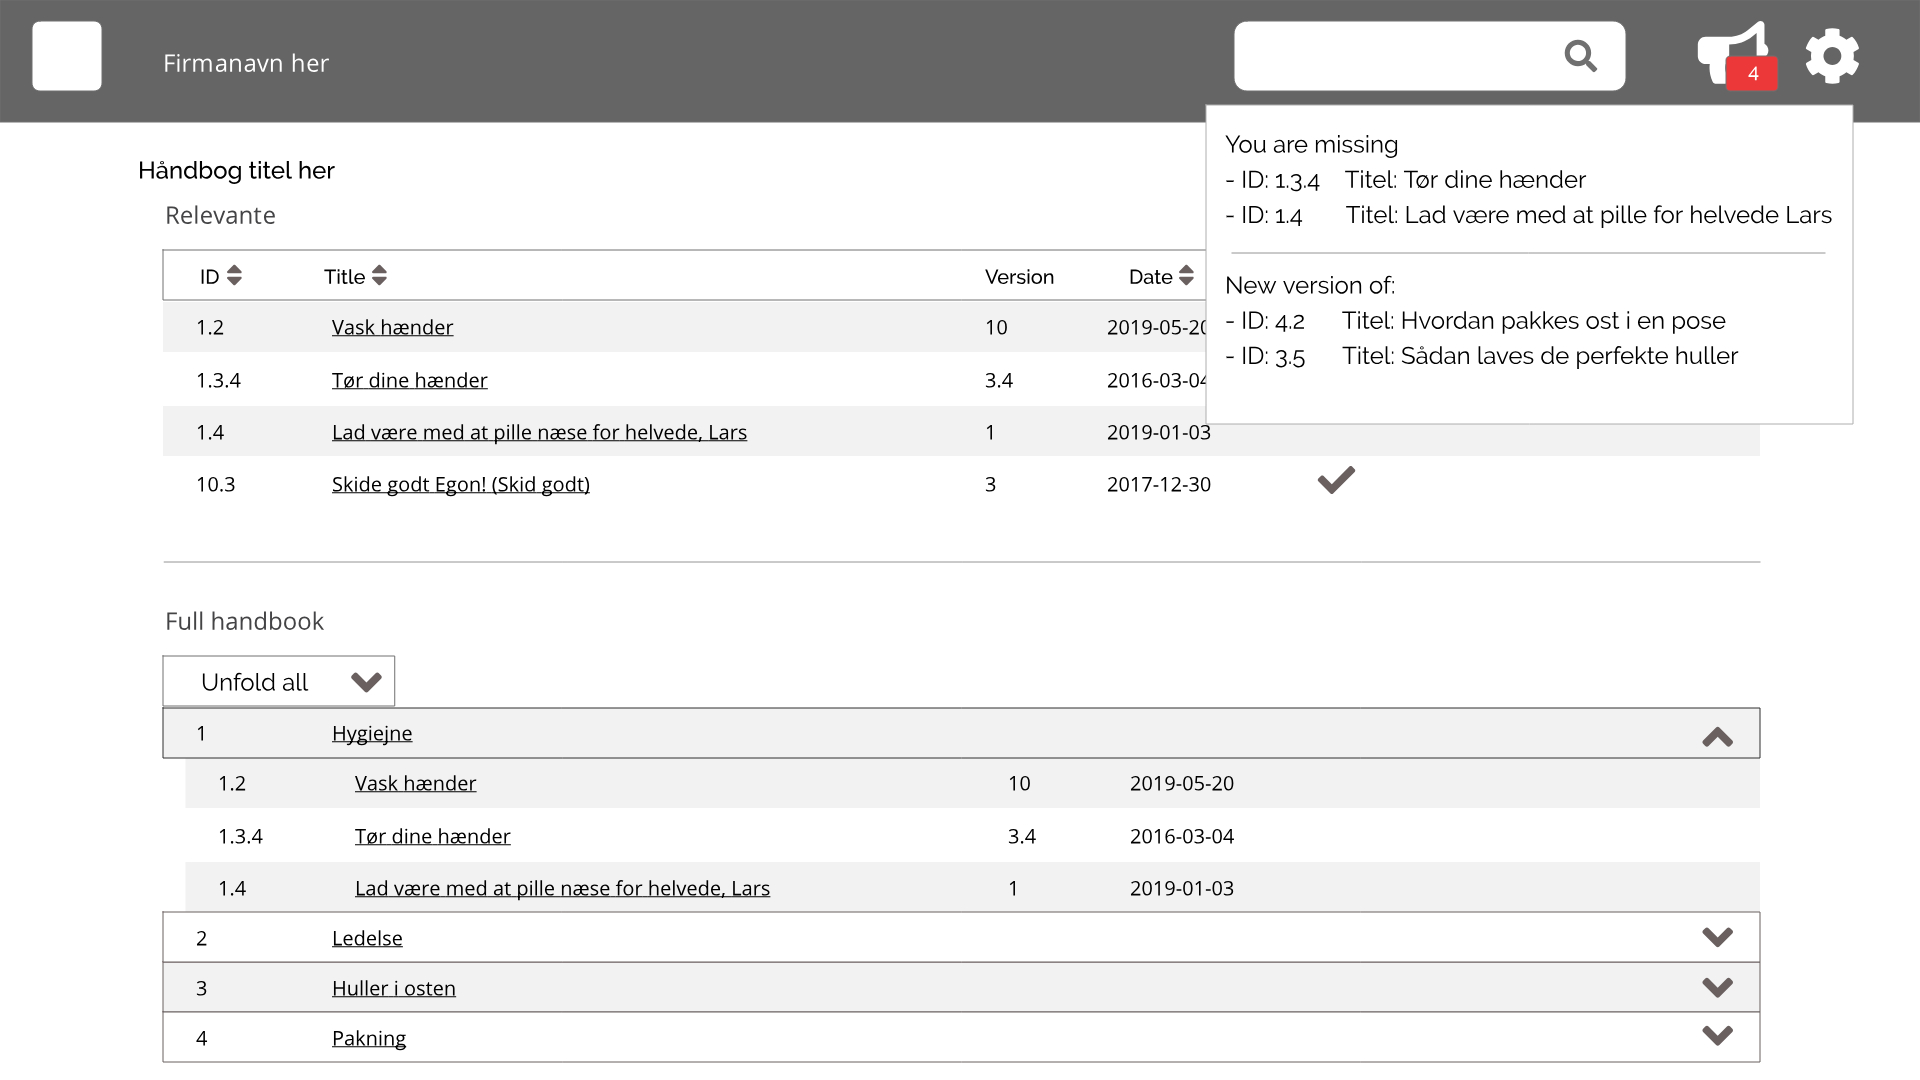
\includegraphics[width=\textwidth]{billeder/iteration2Prototyper/Page_3.jpg}
		\caption{Main interface with notification dropdown}
		\label{fig:4-MainDrop}
	\end{subfigure}
	\quad
	\begin{subfigure}[b]{0.48\textwidth}
		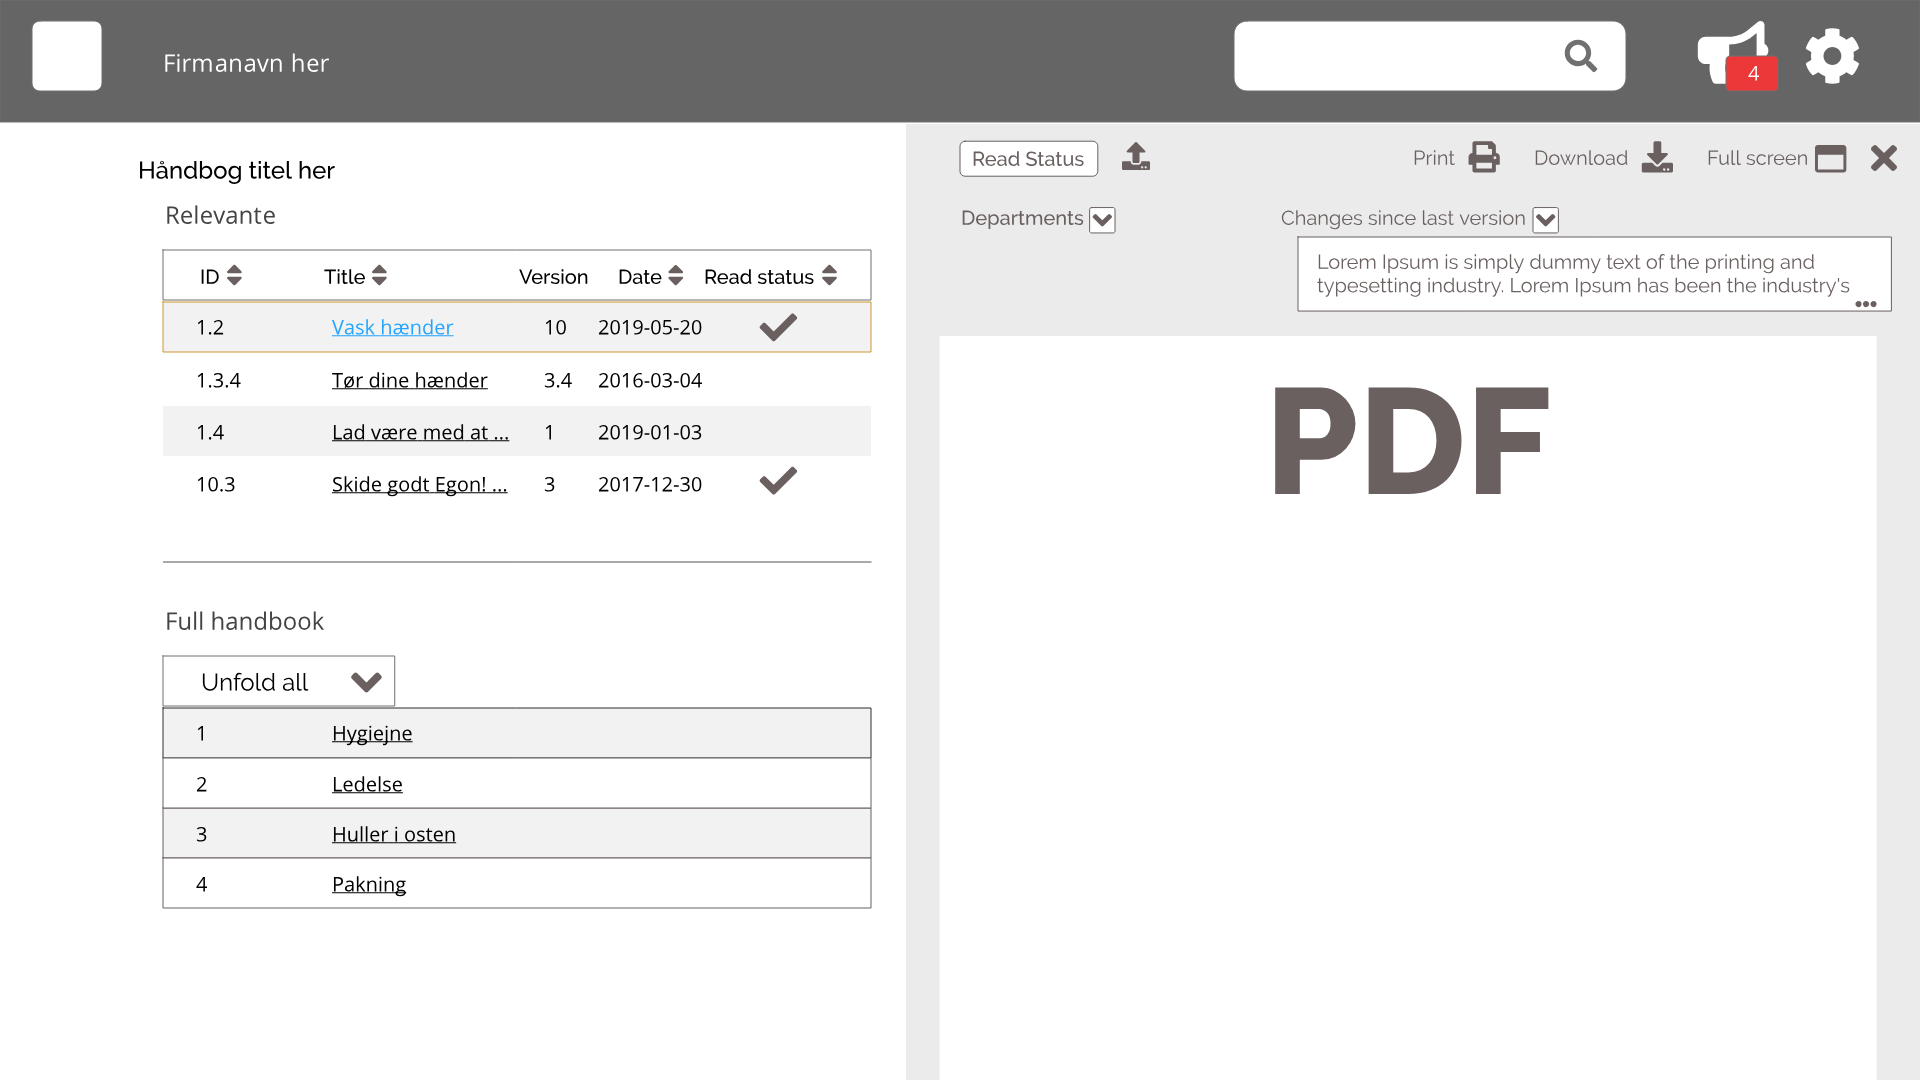
\includegraphics[width=\textwidth]{billeder/iteration2Prototyper/Page_4.jpg}
		\caption{Half document preview}
		\label{fig:4-DocPreviewHalf}
	\end{subfigure}
\end{figure}
\begin{figure}[H]\ContinuedFloat
	\centering
	\begin{subfigure}[b]{0.48\textwidth}
		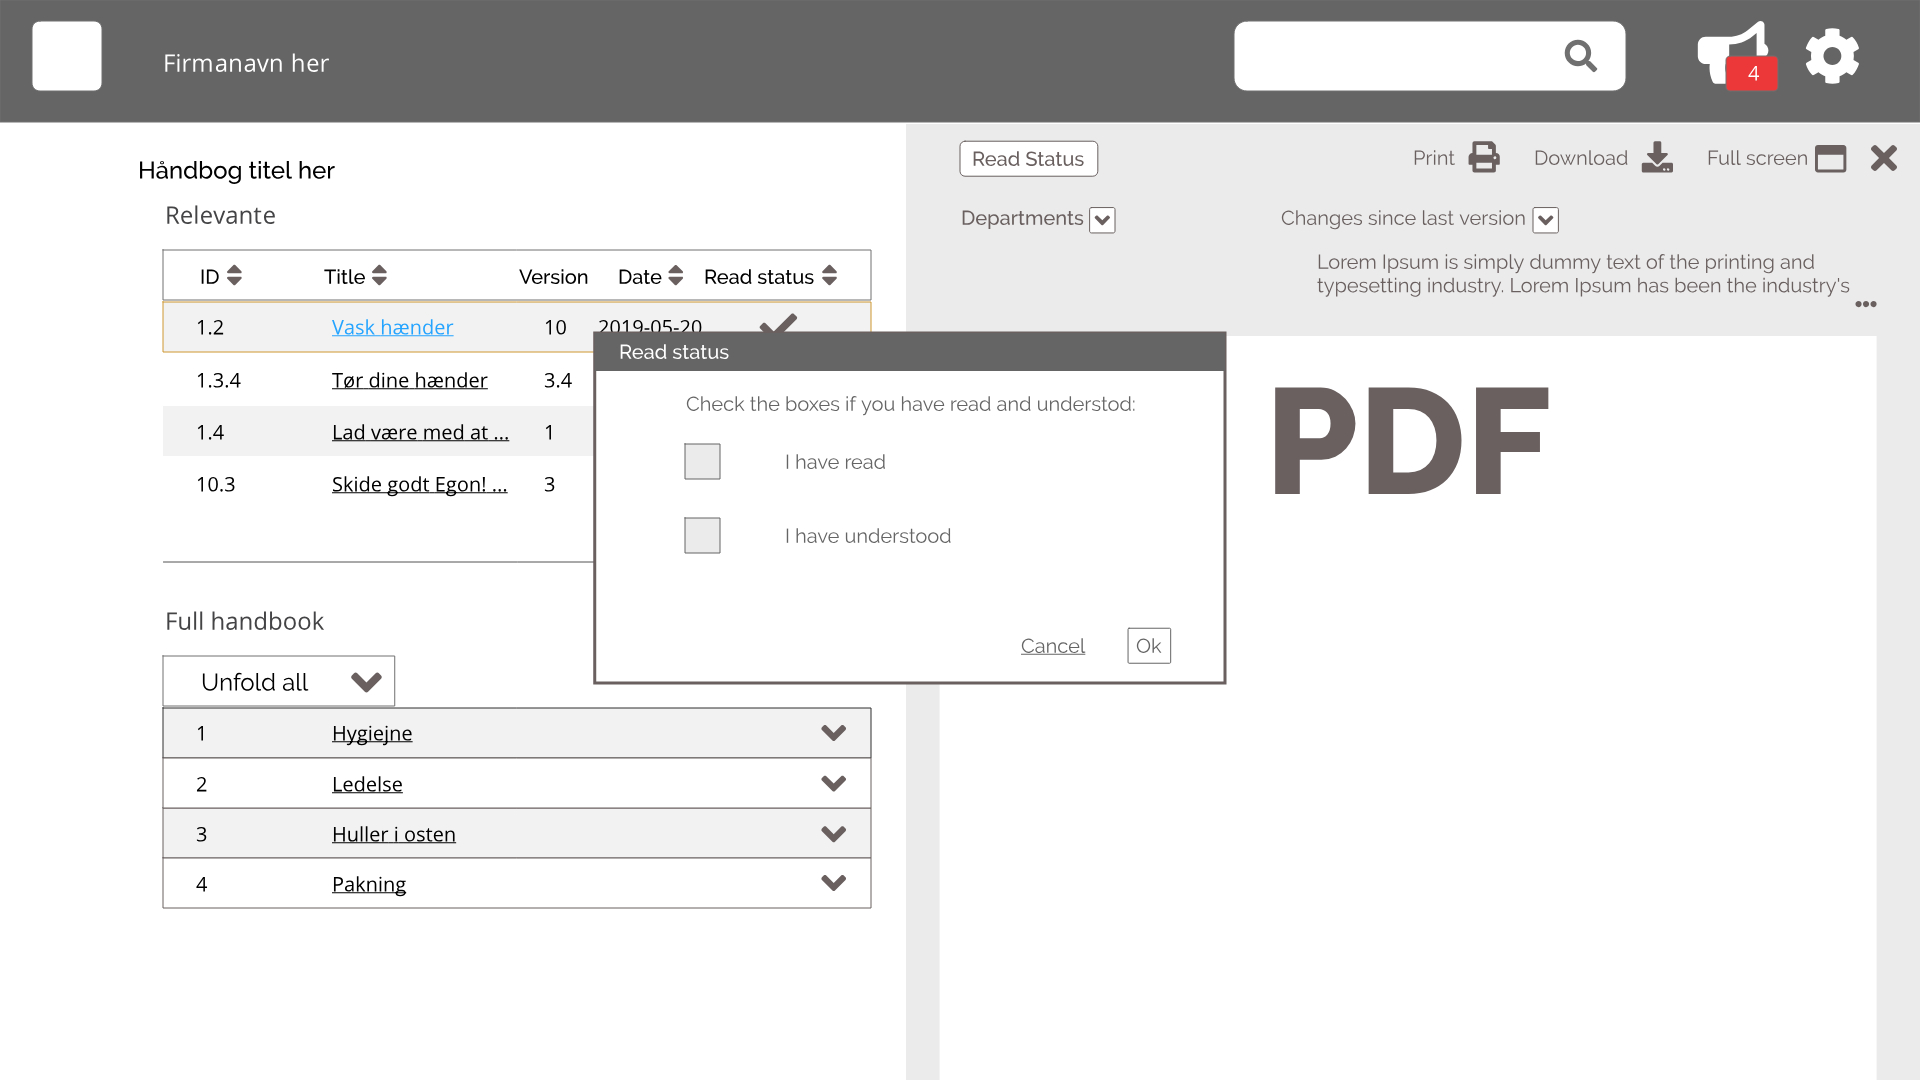
\includegraphics[width=\textwidth]{billeder/iteration2Prototyper/Page_5.jpg}
		\caption{Read status pop-up}
		\label{fig:4-Read}
	\end{subfigure}
	\quad
	\begin{subfigure}[b]{0.48\textwidth}
		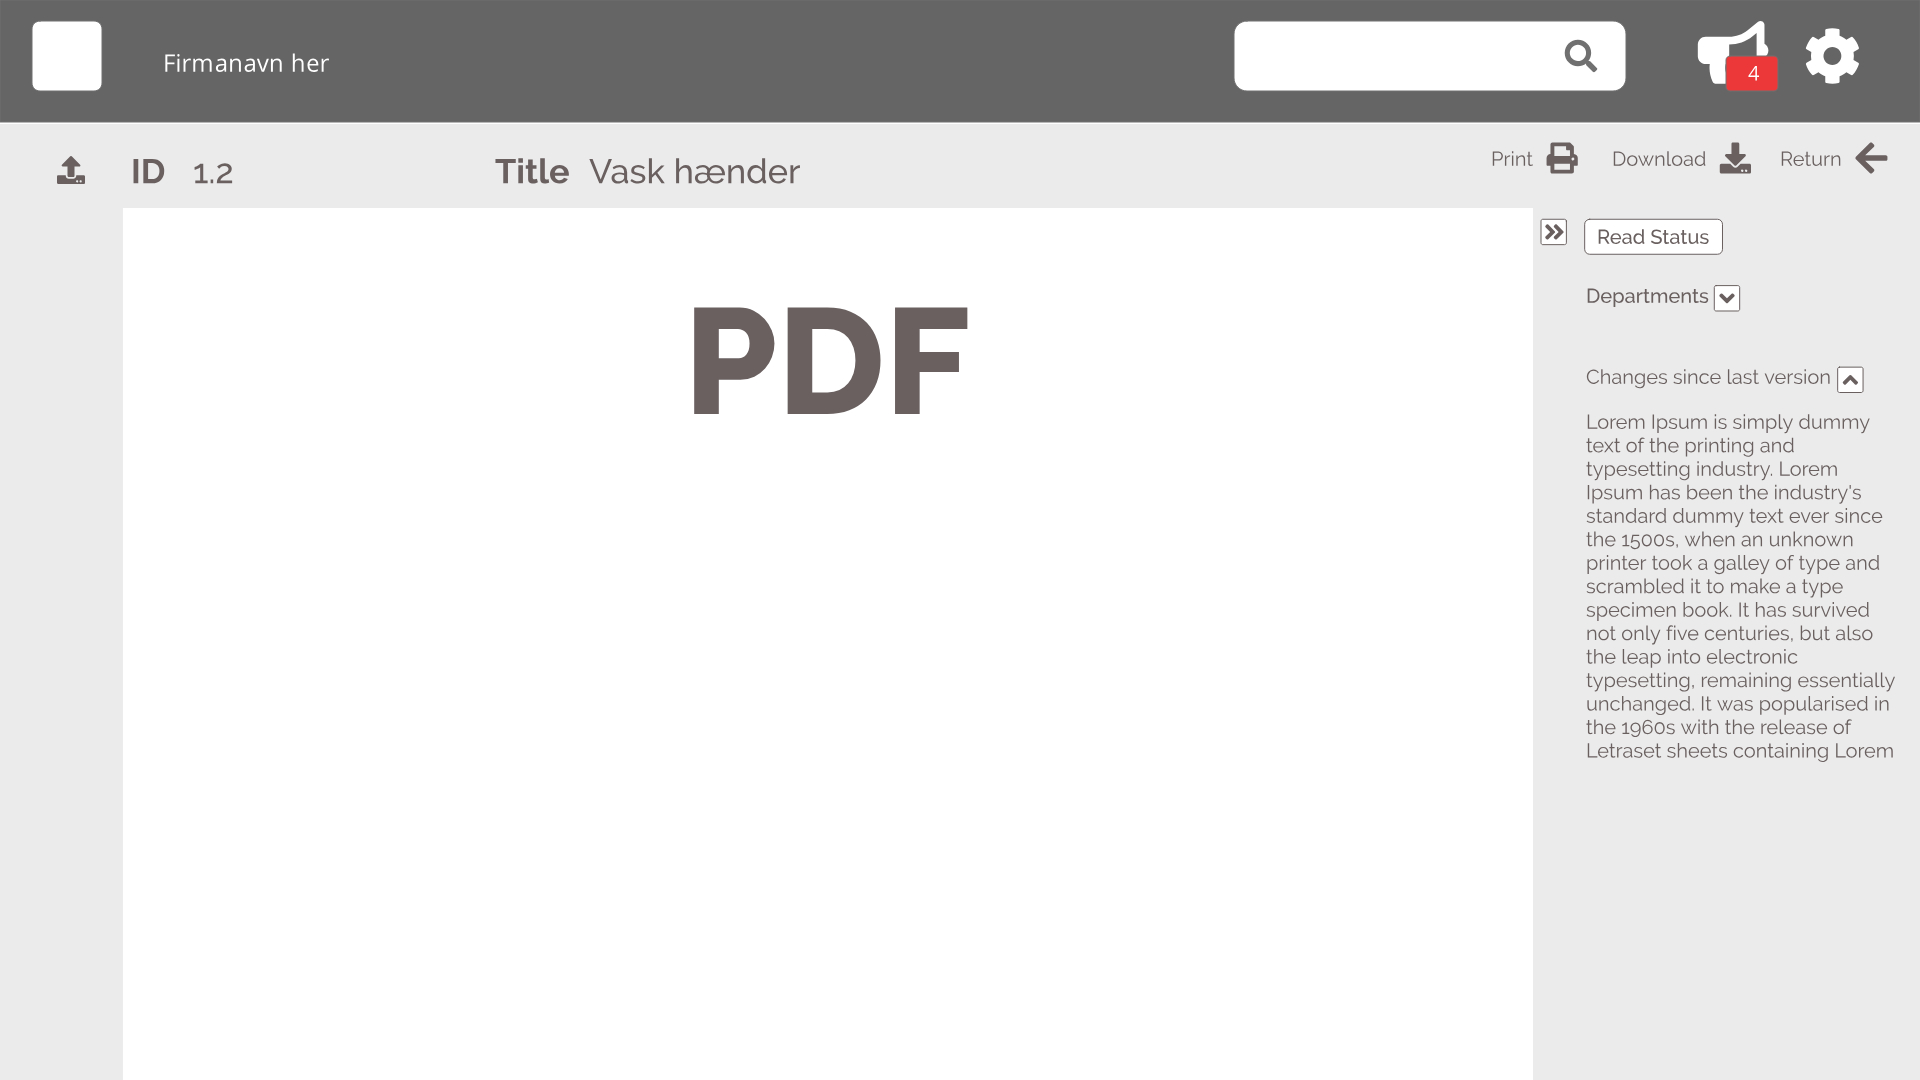
\includegraphics[width=\textwidth]{billeder/iteration2Prototyper/Page_6.jpg}
		\caption{Full document preview}
		\label{fig:4-DocPrevieFull}
	\end{subfigure}
	\caption{Interface design from Mock-up}\label{fig:4-MockUp}
\end{figure}

\section{Main interfaces from prototype for fourth meeting with Ipsen}\label{sec:2prototype}

\chapter{Third Iteration Prototypes} \label{chap:3-Prototypes}
\section{Mockup Continued Development}\label{sec:2Mock}
%Første Blok
\begin{figure}[H]
	\centering
	\begin{subfigure}[b]{0.48\textwidth}
		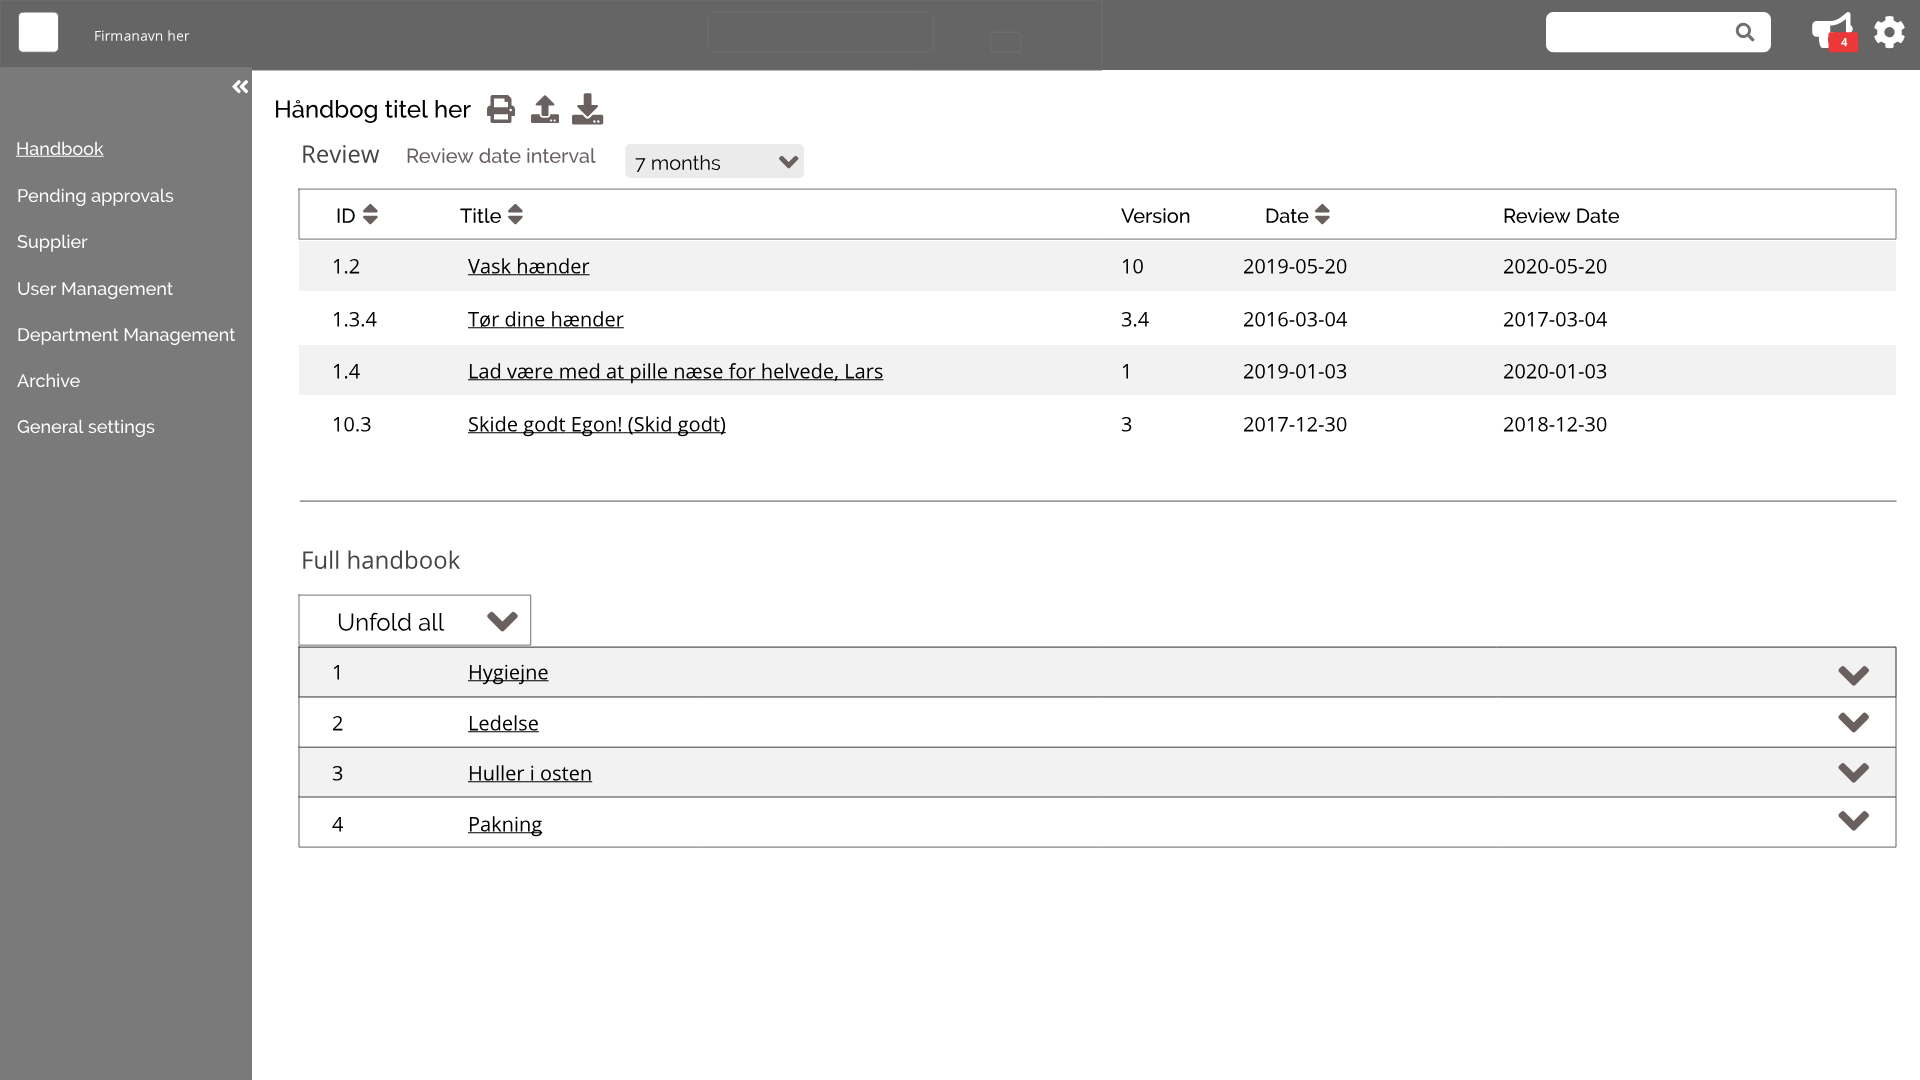
\includegraphics[width=\textwidth]{billeder/iteration3Prototyper/Page_11.jpg}
		\caption{Administrator's main interface 1}
		\label{fig:5-Main1}
	\end{subfigure}
	\quad
	\begin{subfigure}[b]{0.48\textwidth}
		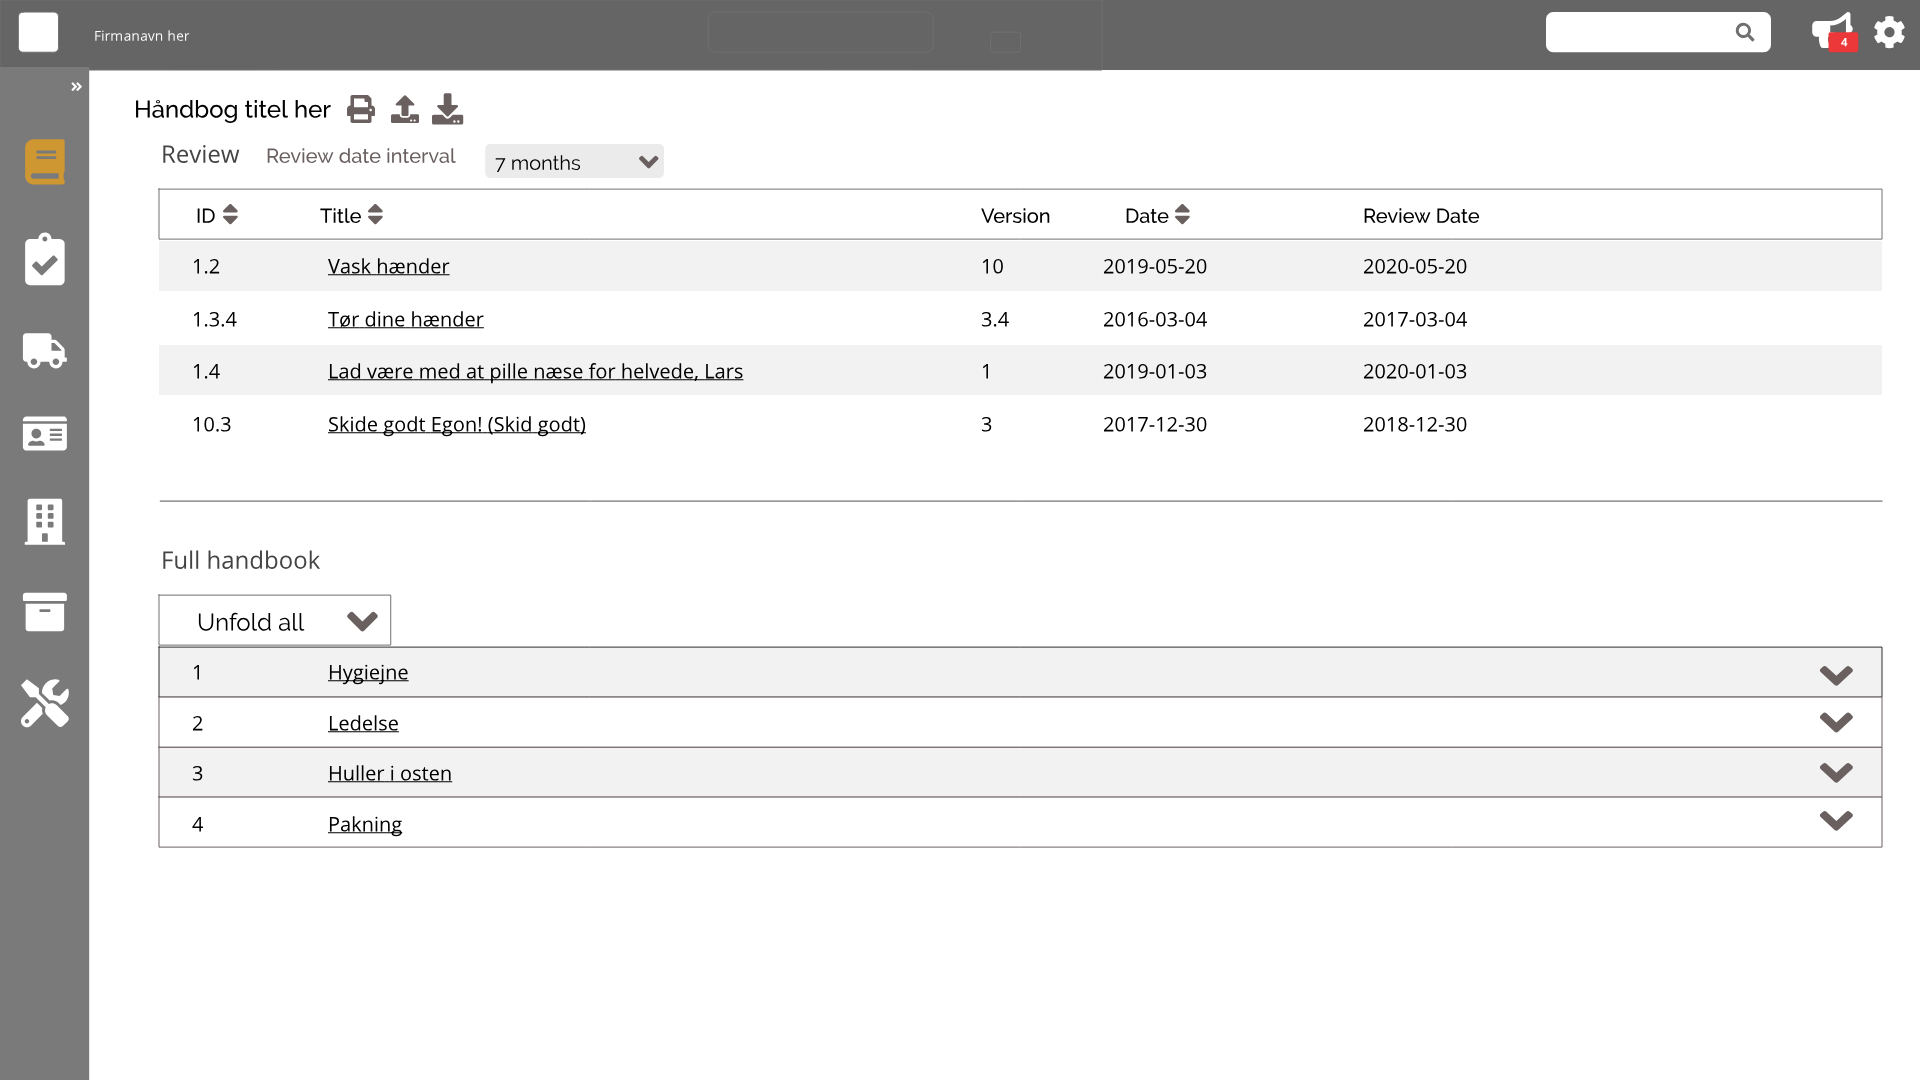
\includegraphics[width=\textwidth]{billeder/iteration3Prototyper/Page_13.jpg}
		\caption{Administrator's main interface 2}
		\label{fig:5-Main2}
	\end{subfigure}
\end{figure}
\begin{figure}[H]\ContinuedFloat
	\centering
	\begin{subfigure}[b]{0.48\textwidth}
		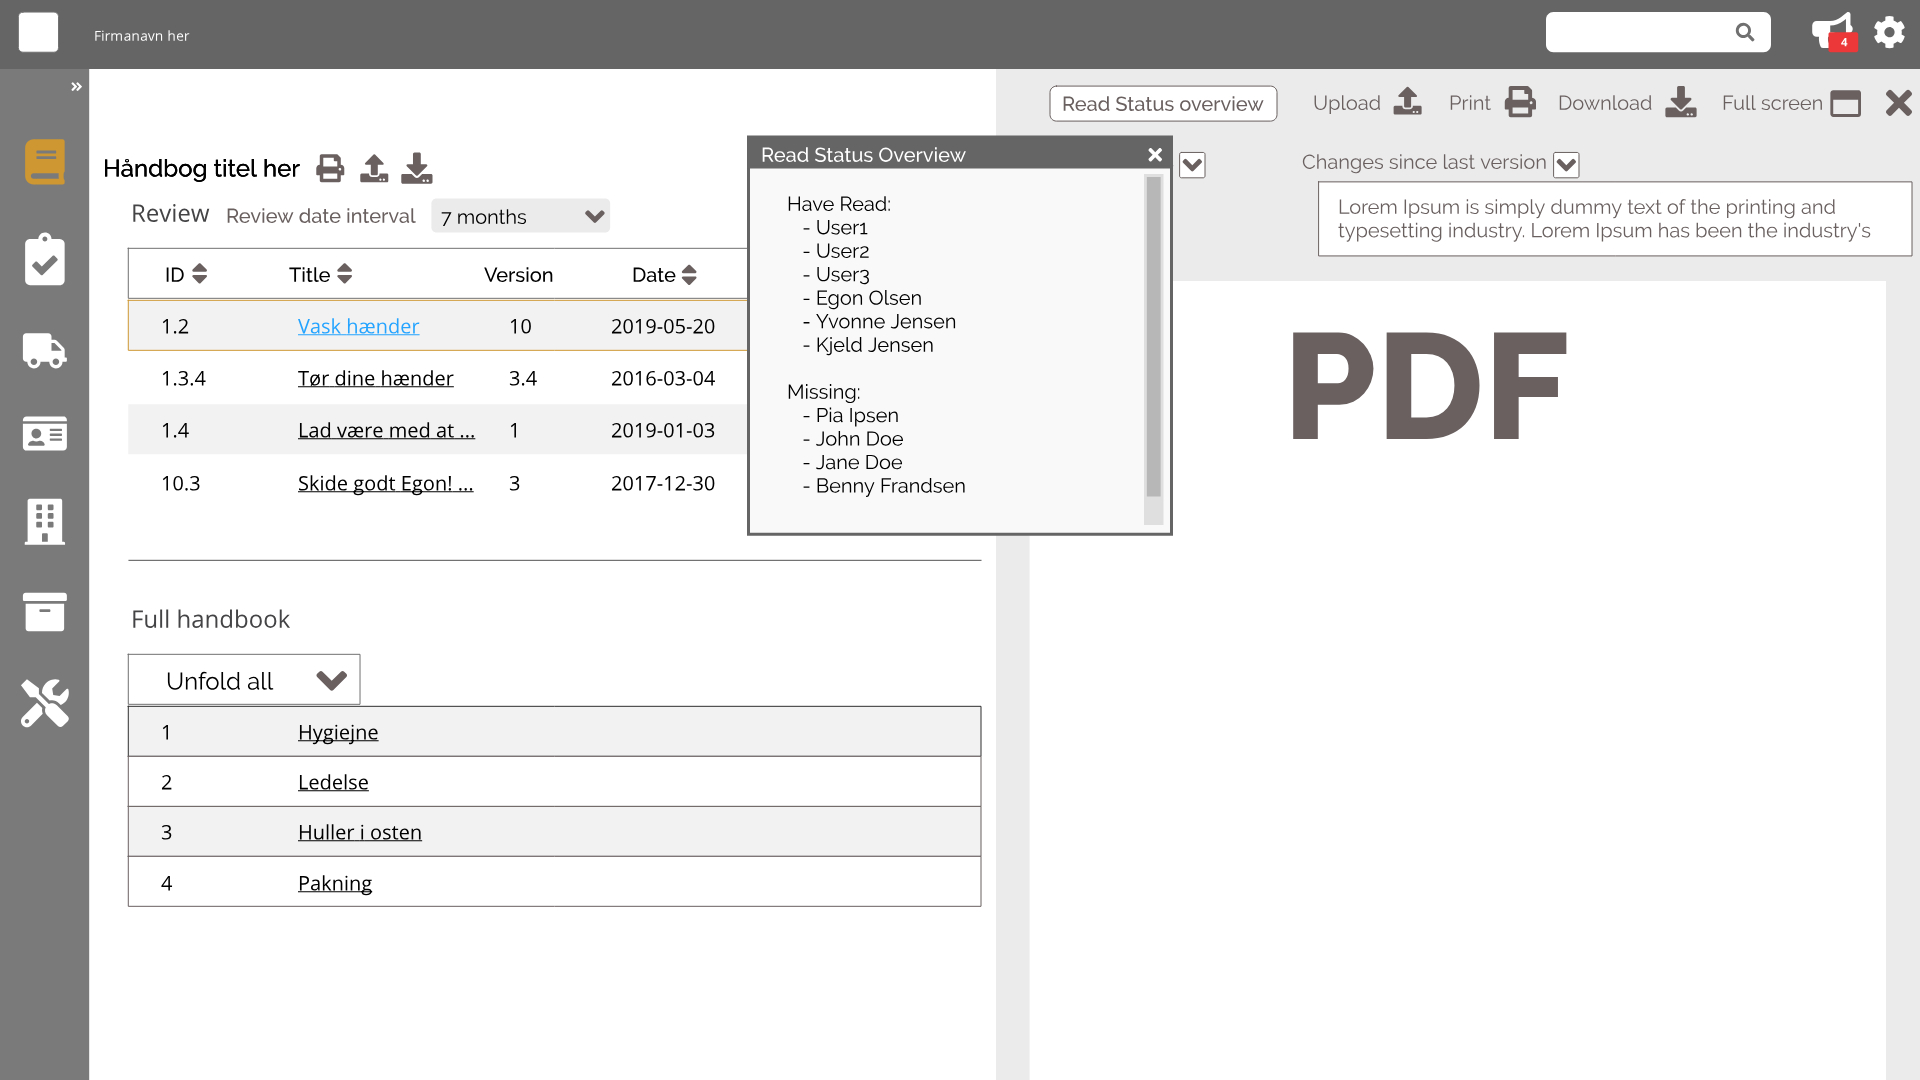
\includegraphics[width=\textwidth]{billeder/iteration3Prototyper/Page_15.jpg}
		\caption{Document preview and read status overview}
		\label{fig:5-PreviewRead}
	\end{subfigure}
	\quad
	\begin{subfigure}[b]{0.48\textwidth}
		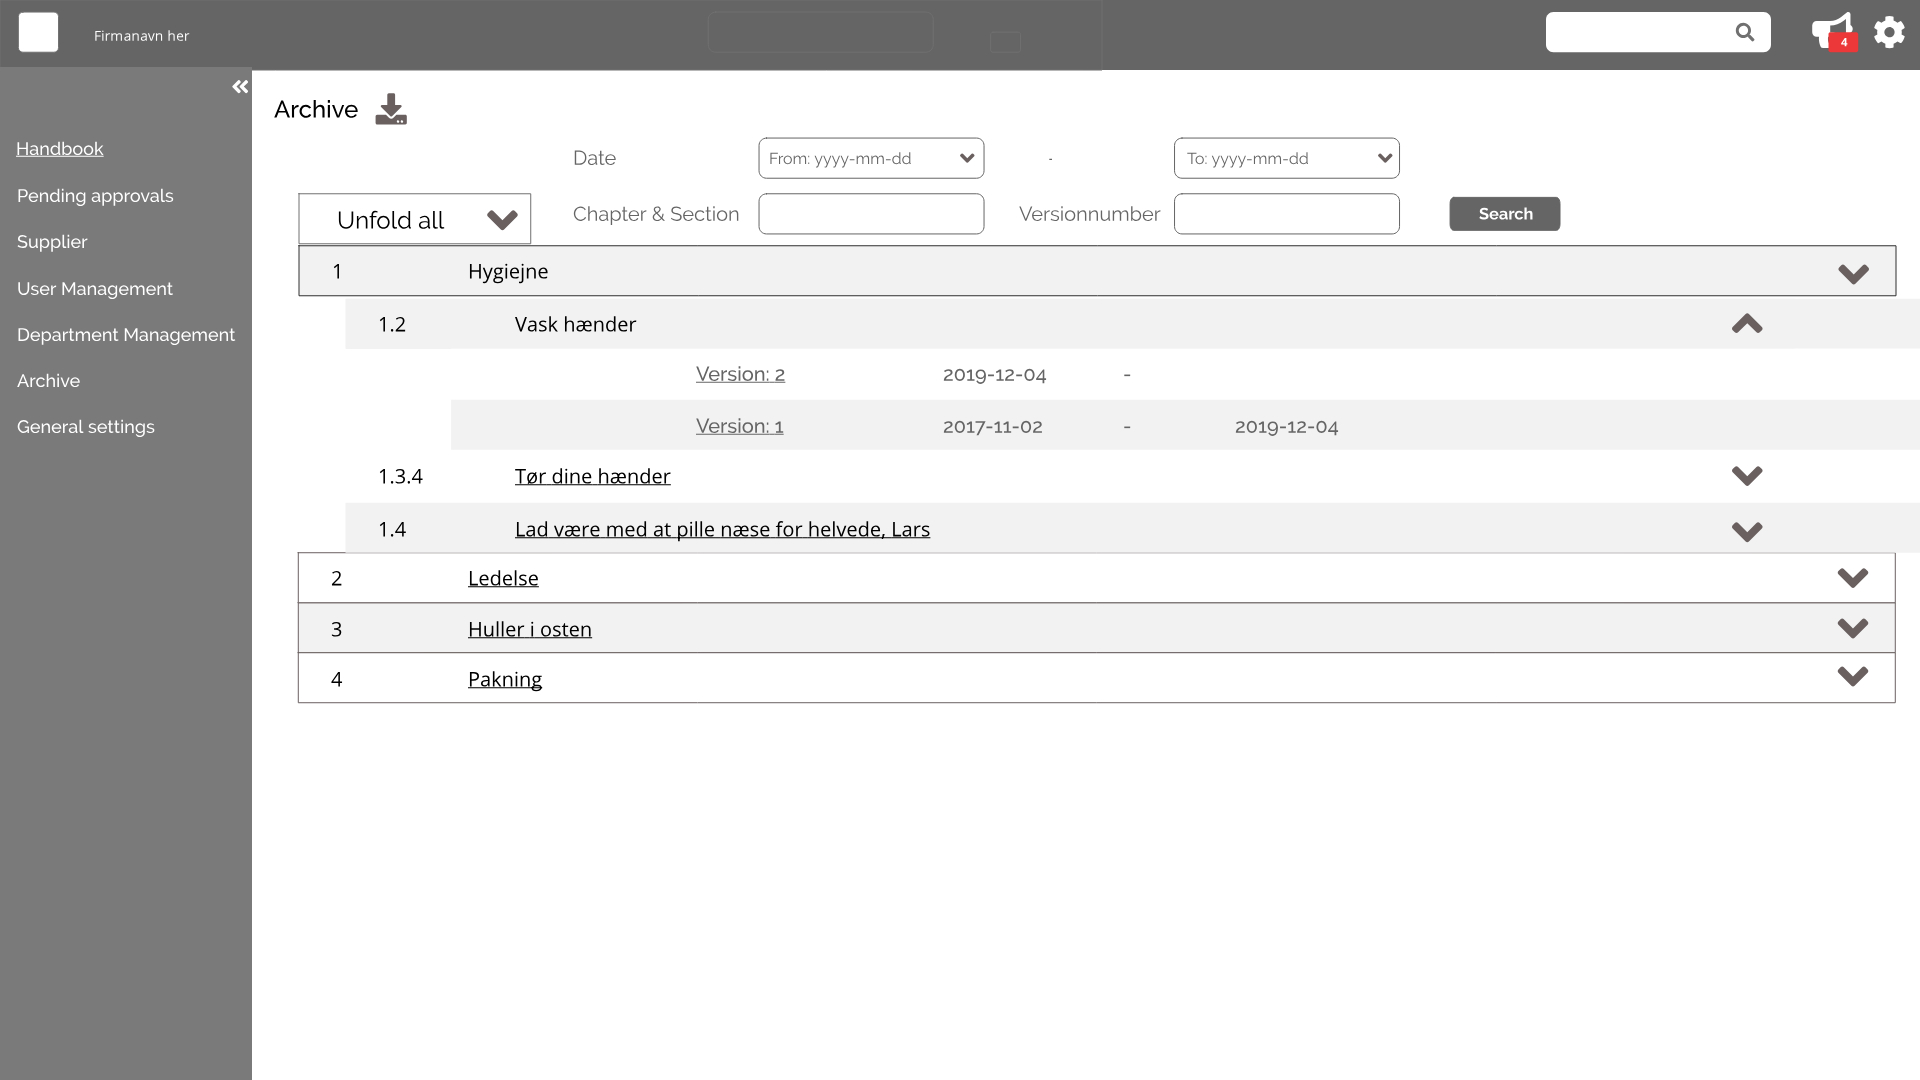
\includegraphics[width=\textwidth]{billeder/iteration3Prototyper/Page_16.jpg}
		\caption{Archive main page}
		\label{fig:5-Archive}
	\end{subfigure}
	\caption{Main and archive interface design from mockup}\label{fig:5-GeneralMockUp}
\end{figure}

%Anden blok
\begin{figure}[H]
	\centering
	\begin{subfigure}[b]{0.48\textwidth}
		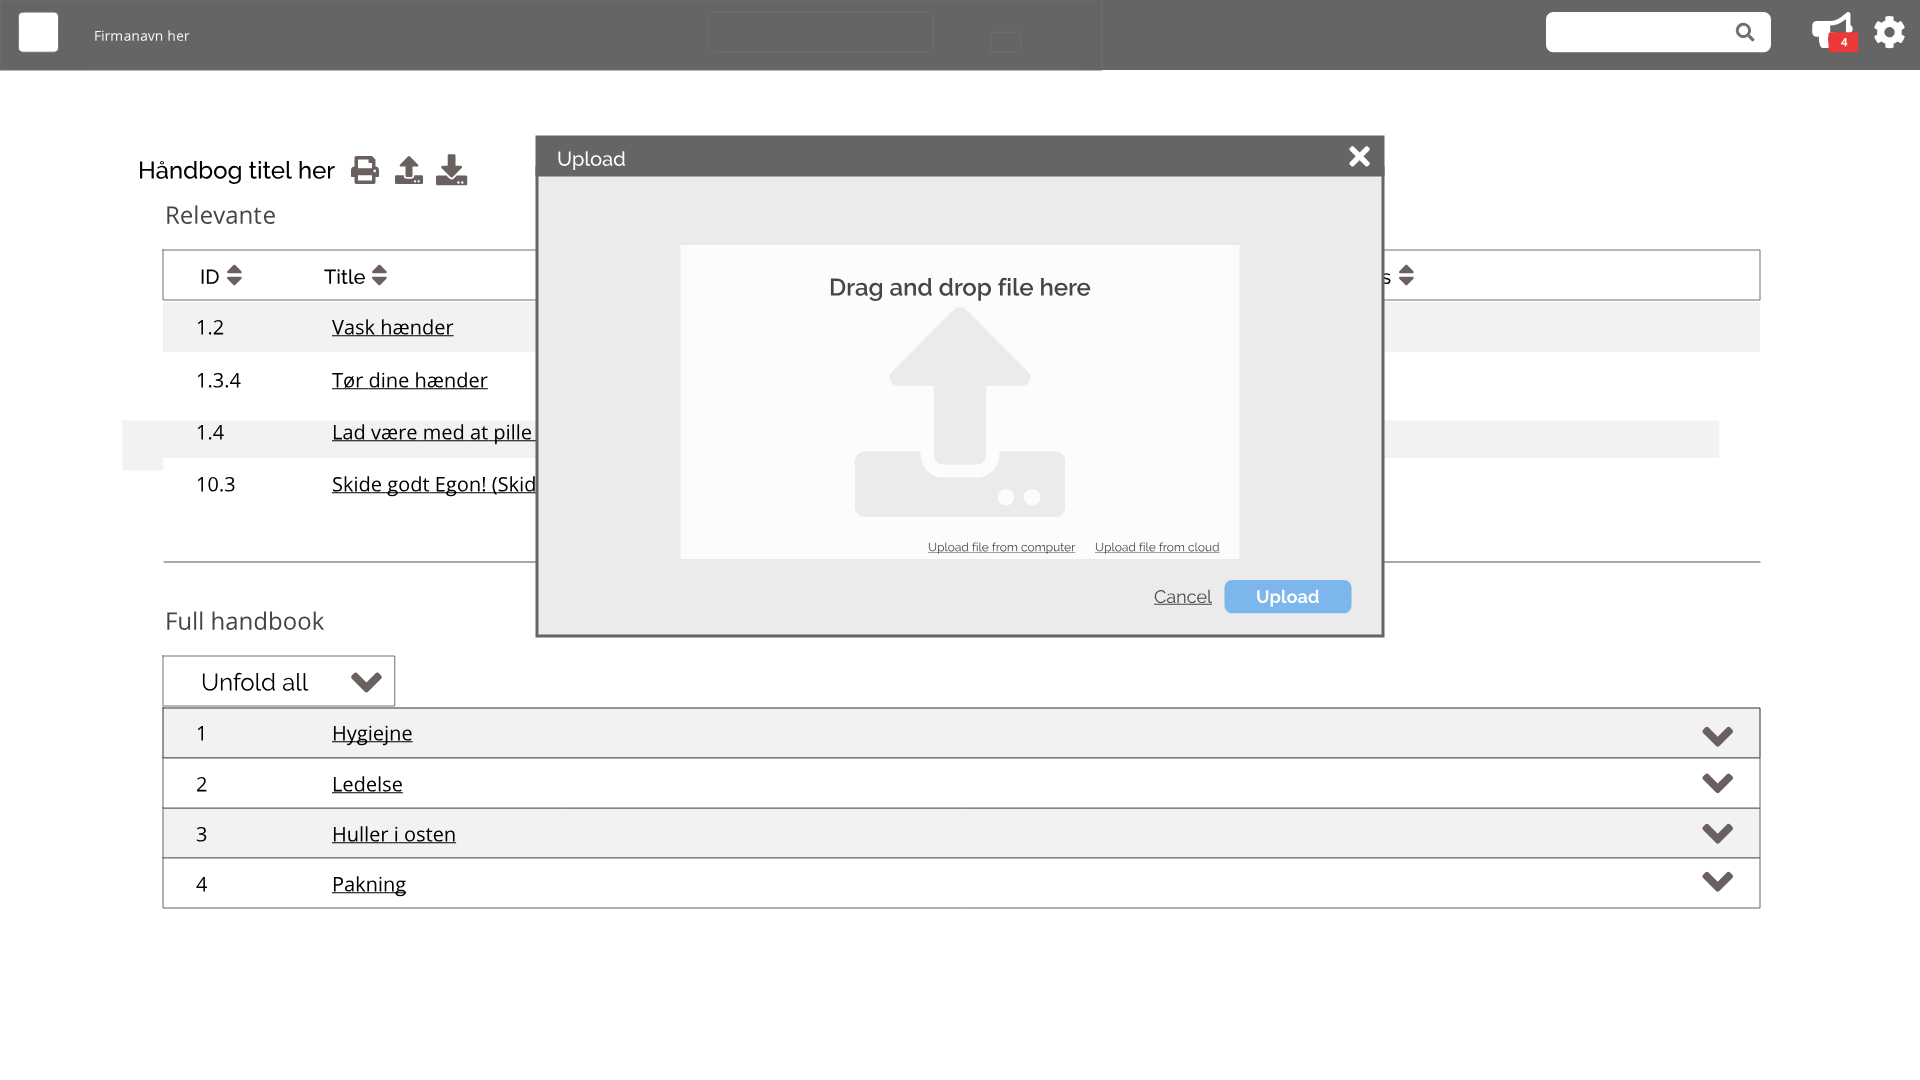
\includegraphics[width=\textwidth]{billeder/iteration3Prototyper/Page_8.jpg}
		\caption{Drag and drop upload}
		\label{fig:5-Upload1}
	\end{subfigure}
	\quad
	\begin{subfigure}[b]{0.48\textwidth}
		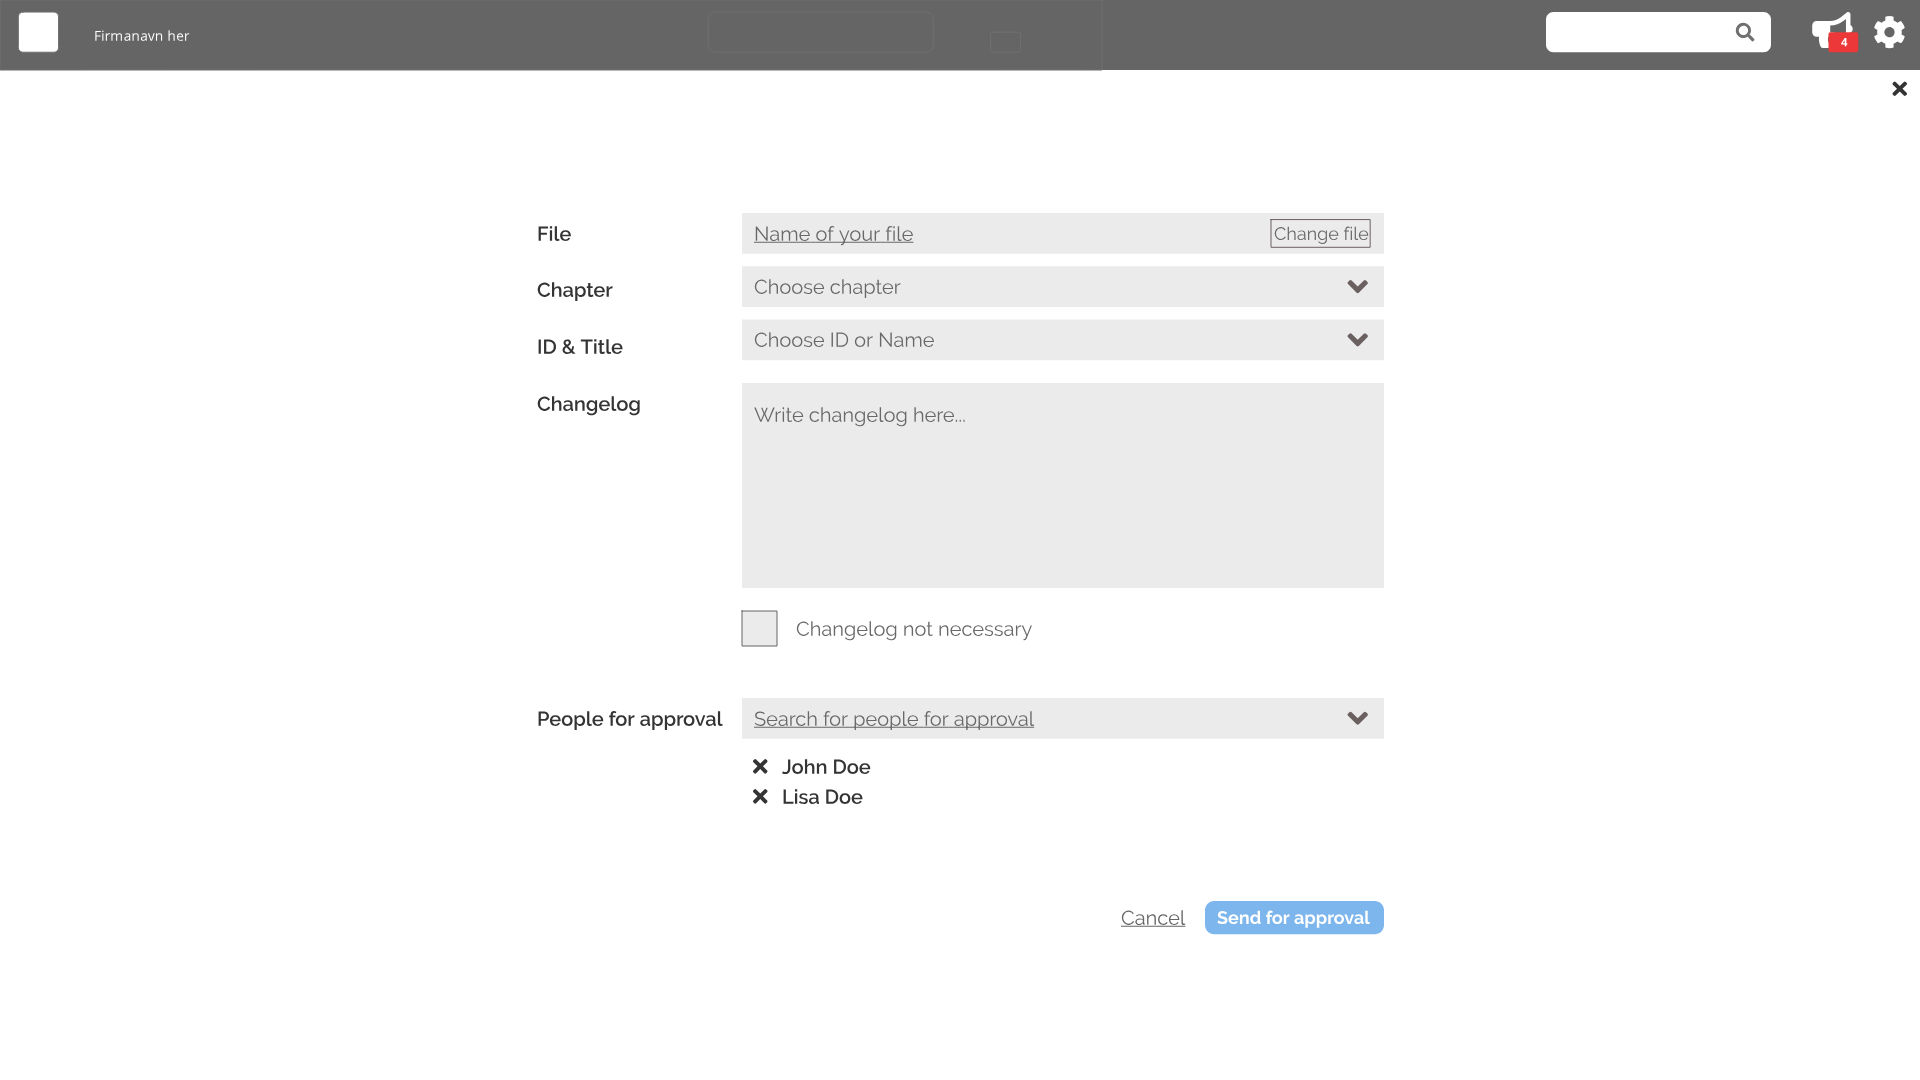
\includegraphics[width=\textwidth]{billeder/iteration3Prototyper/Page_9.jpg}
		\caption{Upload new version or document main interface}
		\label{fig:5-Upload2}
	\end{subfigure}
\end{figure}
\begin{figure}[H]\ContinuedFloat
	\centering
	\begin{subfigure}[b]{0.48\textwidth}
		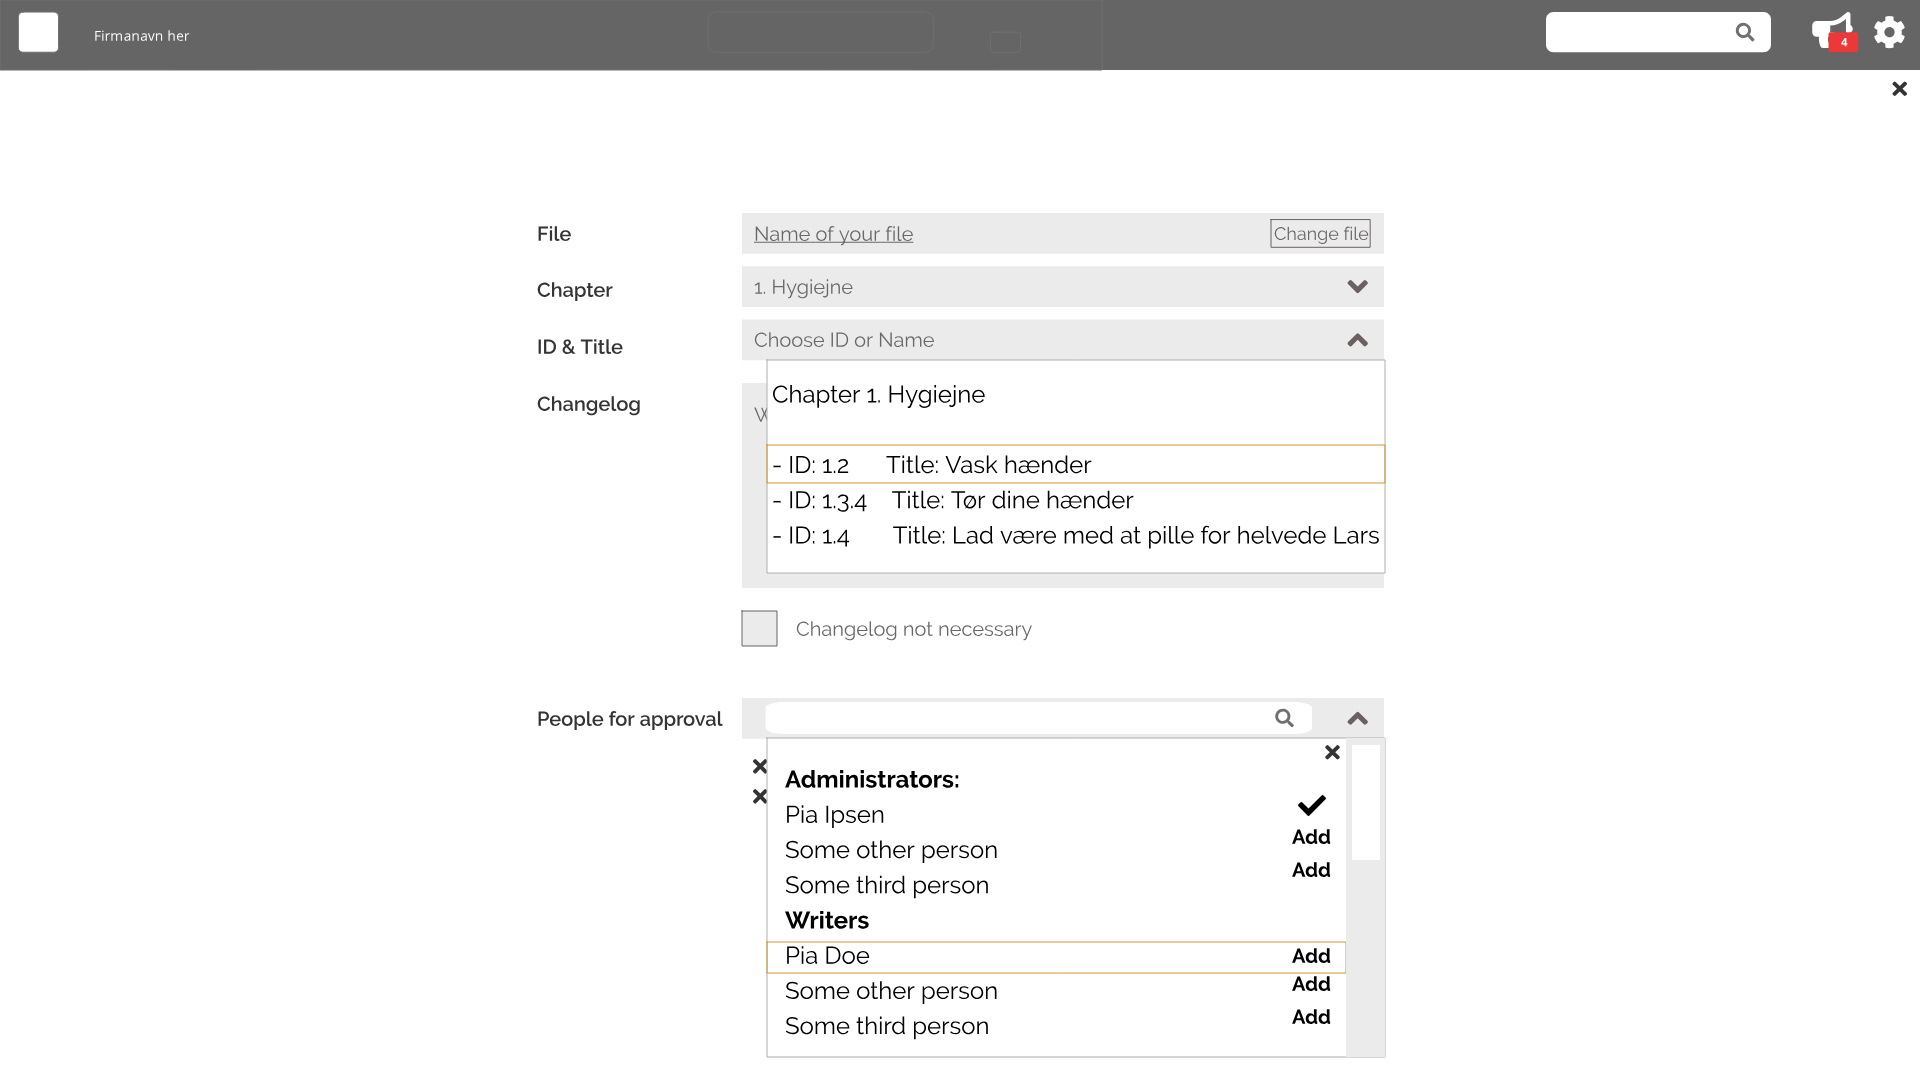
\includegraphics[width=\textwidth]{billeder/iteration3Prototyper/Page_10.jpg}
		\caption{Upload with dropdowns open}
		\label{fig:5-Upload 3}
	\end{subfigure}
	\quad
	\begin{subfigure}[b]{0.48\textwidth}
		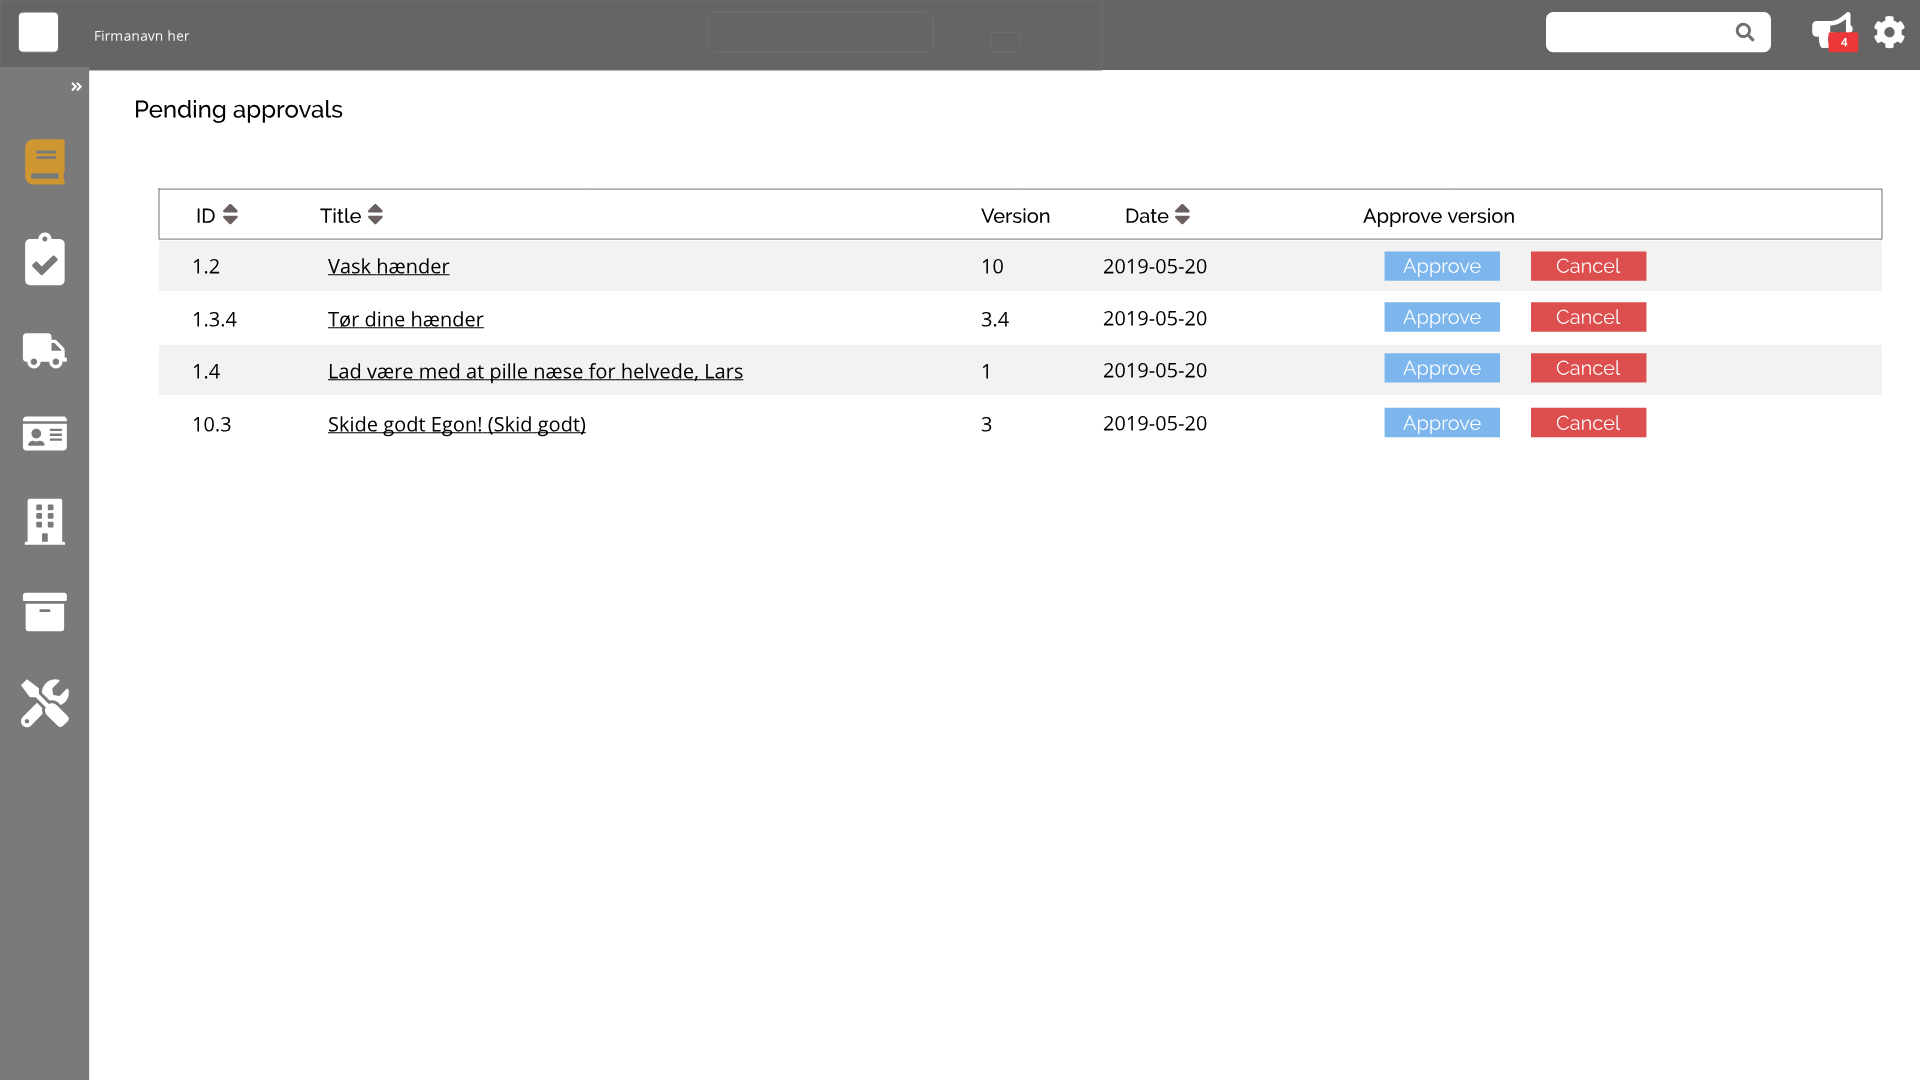
\includegraphics[width=\textwidth]{billeder/iteration3Prototyper/Page_18.jpg}
		\caption{Pending approval main interface}
		\label{fig:5-Approval1}
	\end{subfigure}
\end{figure}
\begin{figure}[H]\ContinuedFloat
	\centering
	\begin{subfigure}[b]{0.48\textwidth}
		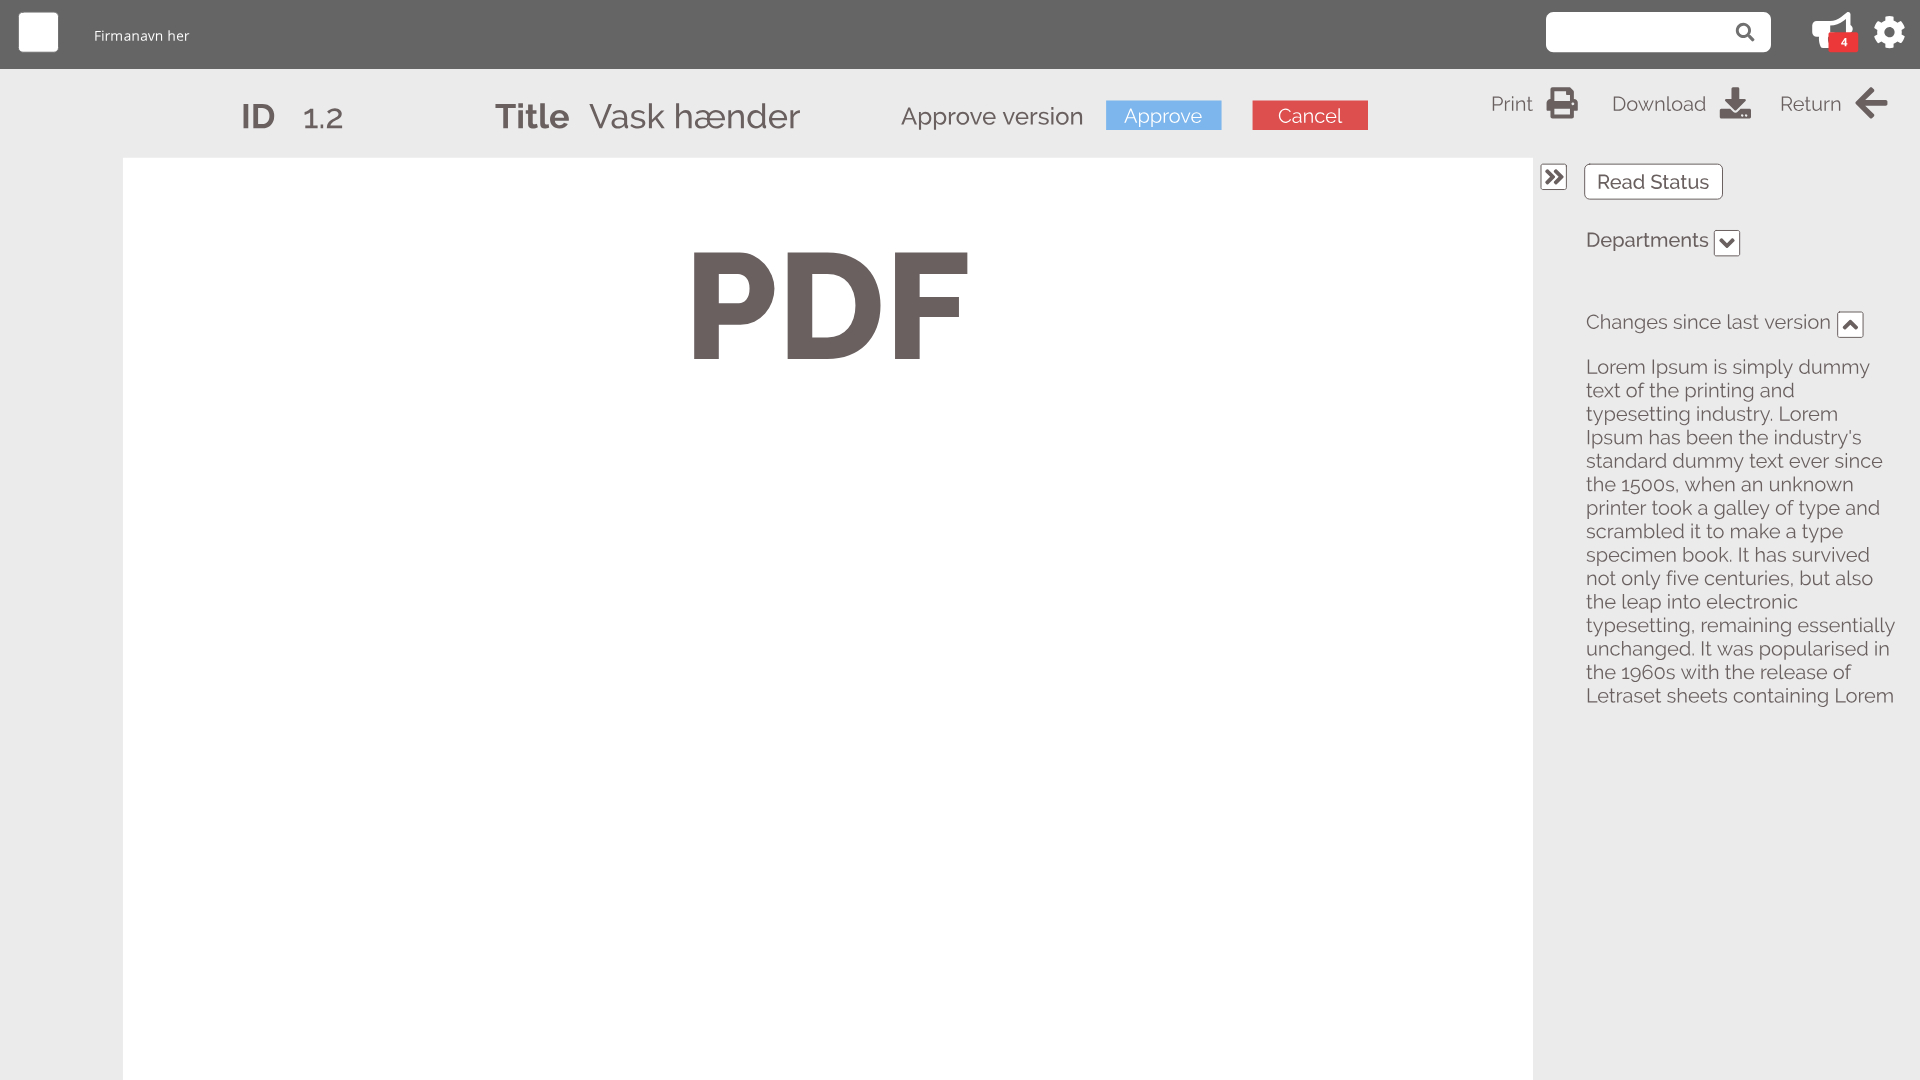
\includegraphics[width=\textwidth]{billeder/iteration3Prototyper/Page_19.jpg}
		\caption{Pending approval preview interface}
		\label{fig:5-Approval2}
	\end{subfigure}
	\caption{Upload and approval main interface design from mockup}\label{fig:5-DocMockUp}
\end{figure}

%Tredje blok
\begin{figure}[H]
	\centering
	\begin{subfigure}[b]{0.48\textwidth}
		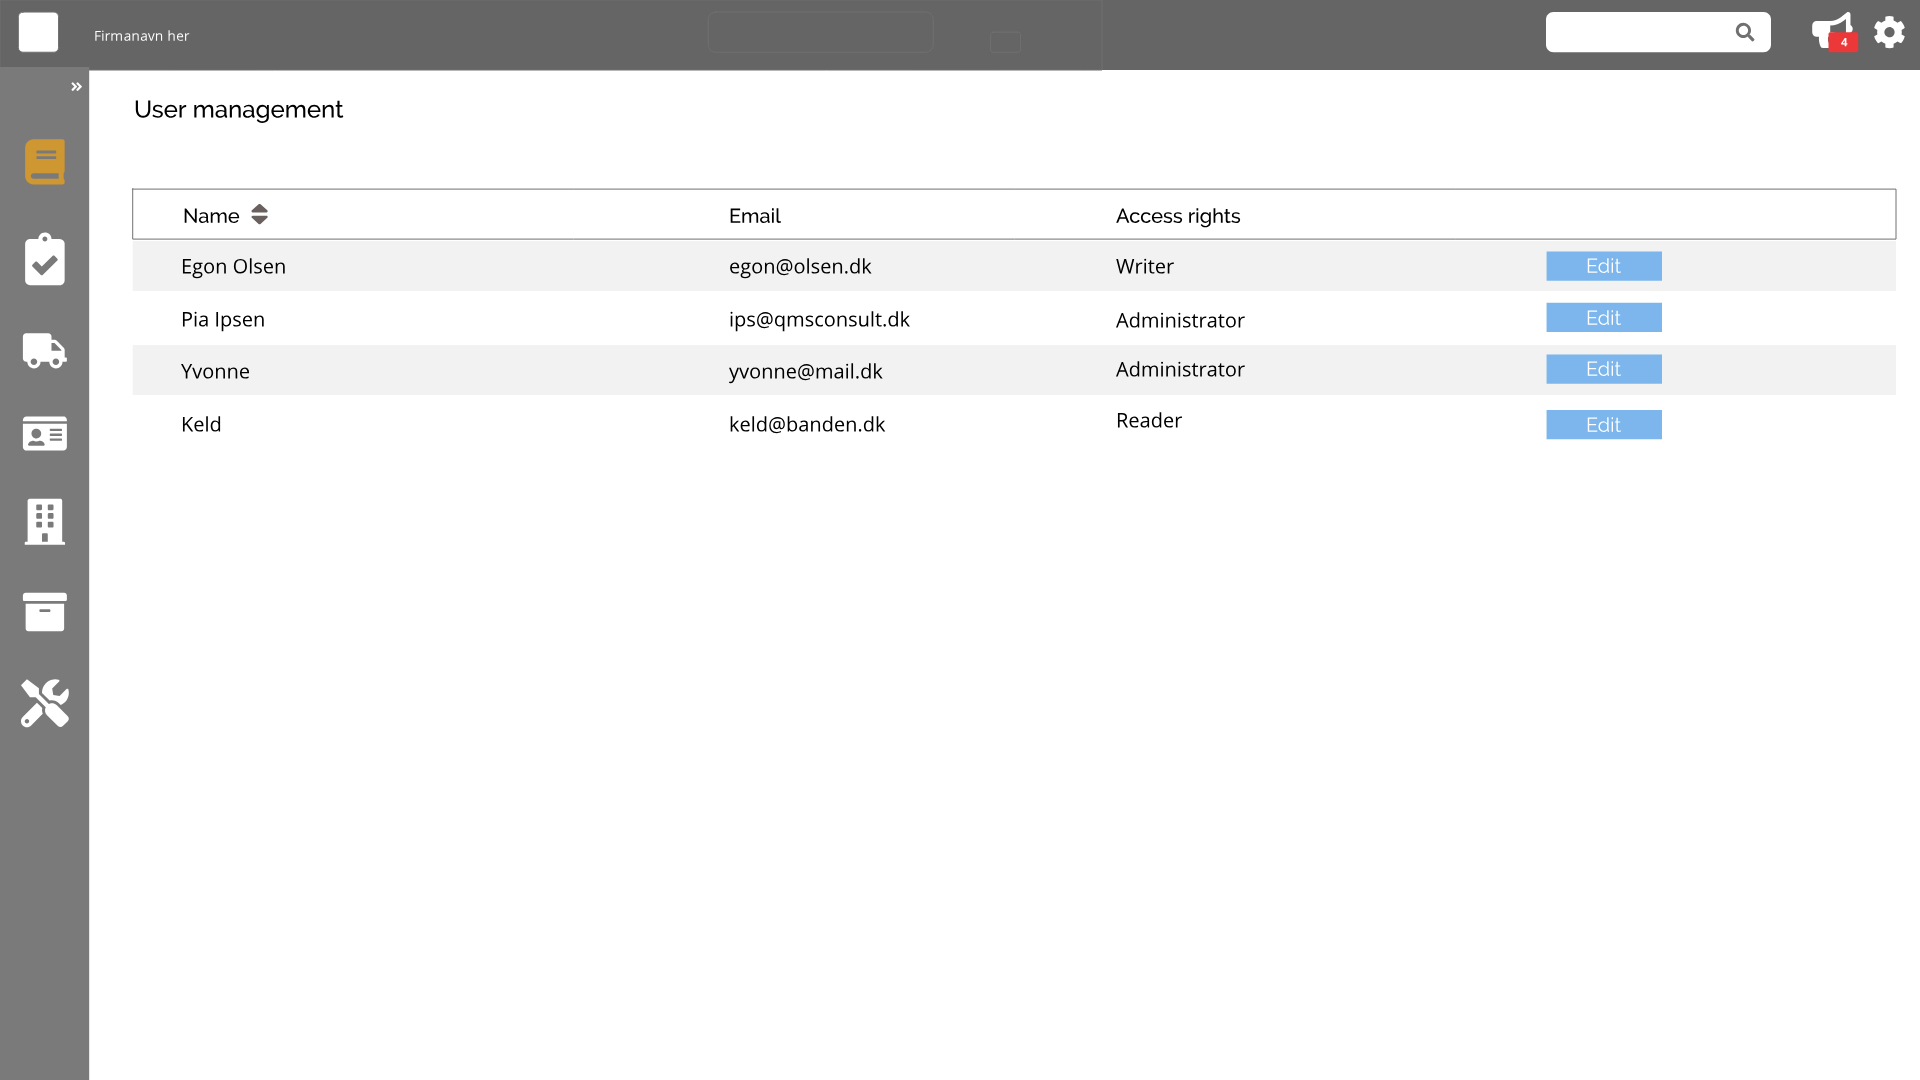
\includegraphics[width=\textwidth]{billeder/iteration3Prototyper/Page_20.jpg}
		\caption{User management main interface}
		\label{fig:5-UserMan}
	\end{subfigure}
	\quad
	\begin{subfigure}[b]{0.48\textwidth}
		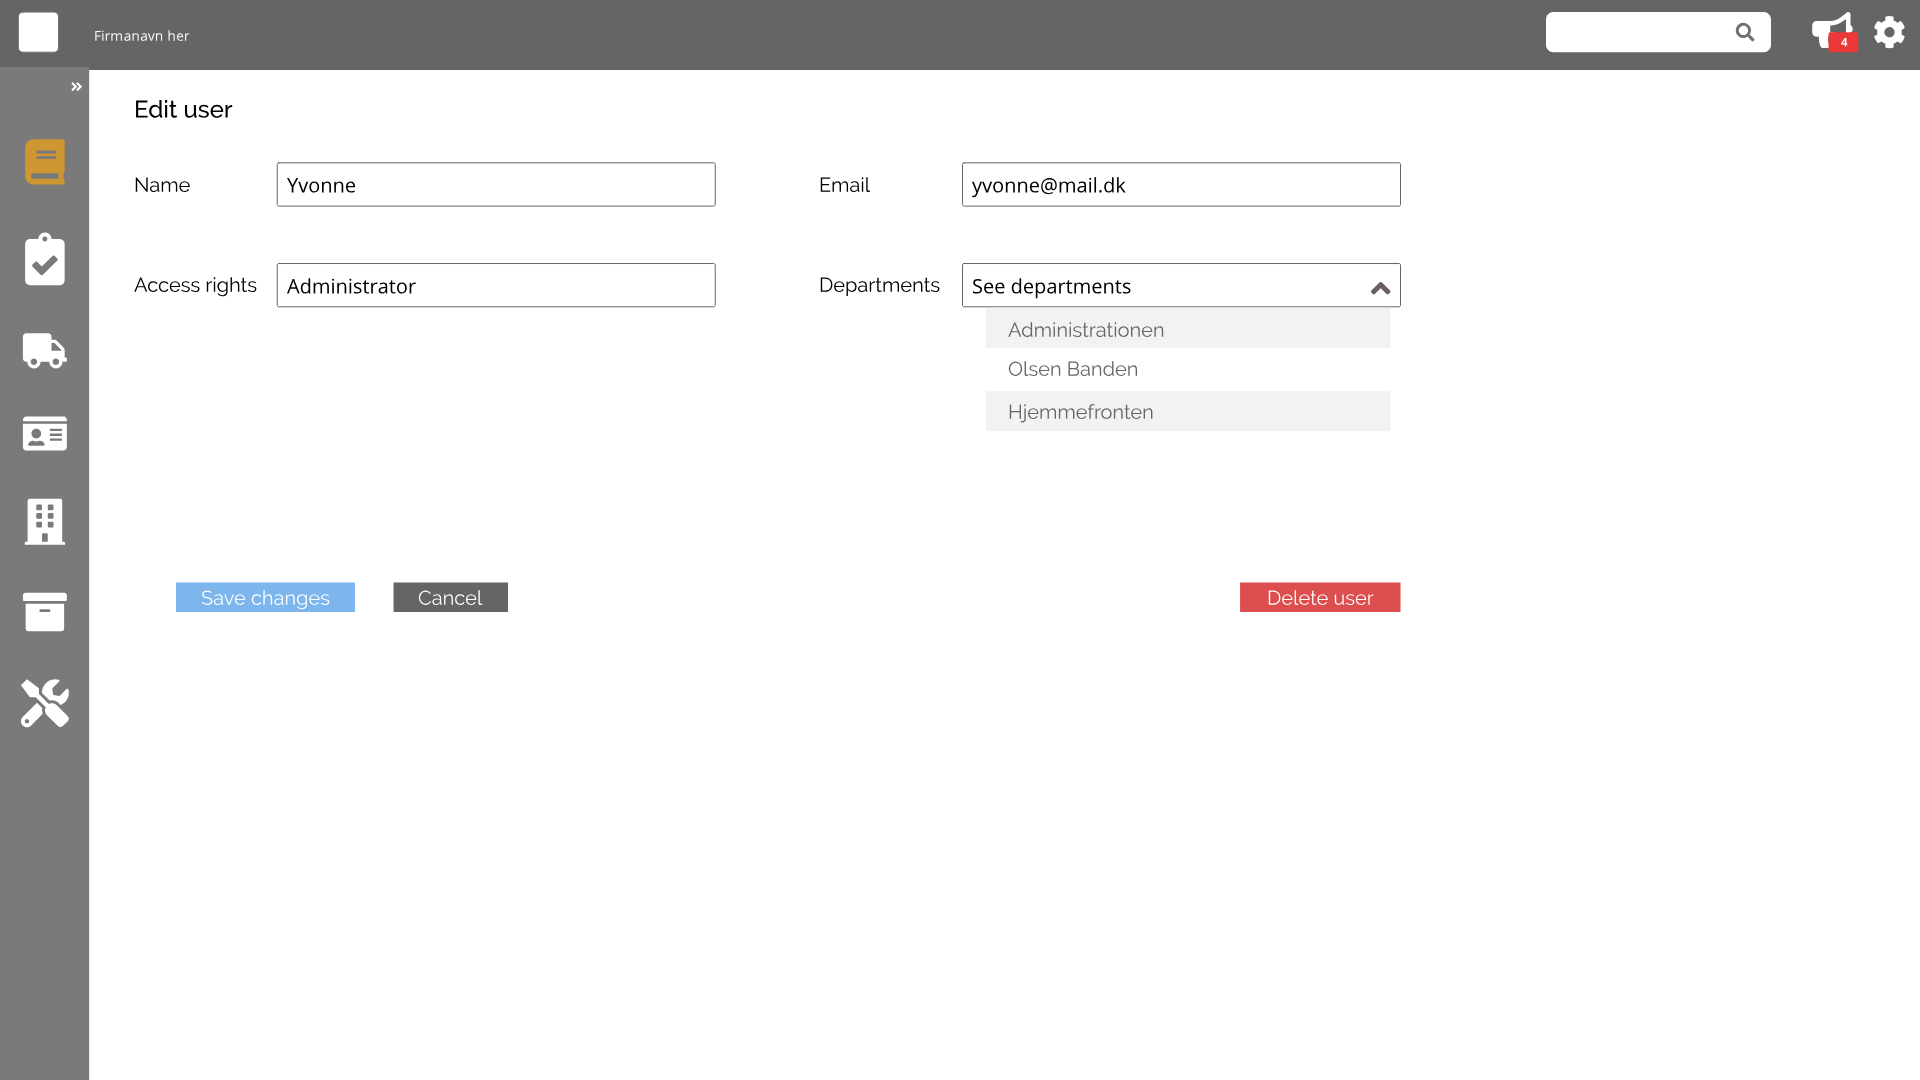
\includegraphics[width=\textwidth]{billeder/iteration3Prototyper/Page_21.jpg}
		\caption{User management edit user interface}
		\label{fig:5-UserManEdit}
	\end{subfigure}
\end{figure}
\begin{figure}[H]\ContinuedFloat
	\centering
	\begin{subfigure}[b]{0.48\textwidth}
		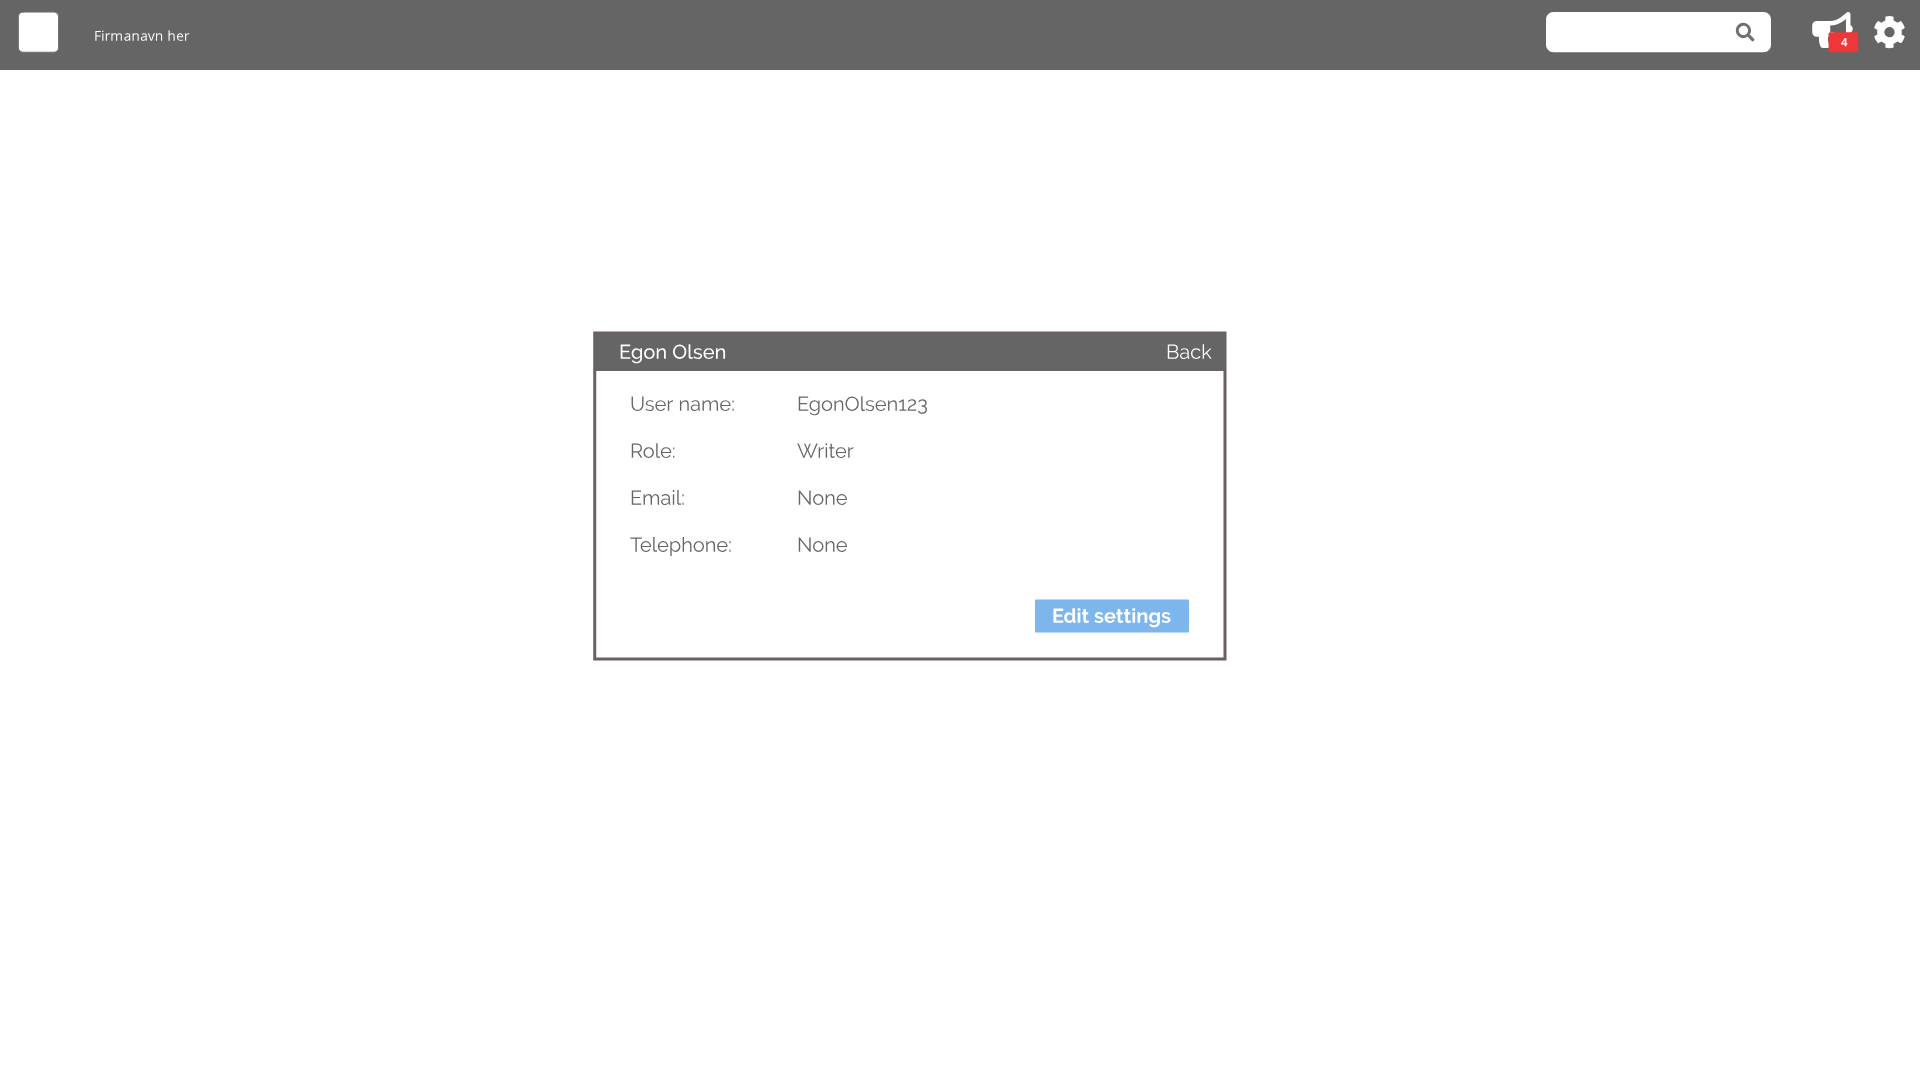
\includegraphics[width=\textwidth]{billeder/iteration3Prototyper/Page_27.jpg}
		\caption{Profile setting main interface}
		\label{fig:5-Profile}
	\end{subfigure}
	\quad
	\begin{subfigure}[b]{0.48\textwidth}
		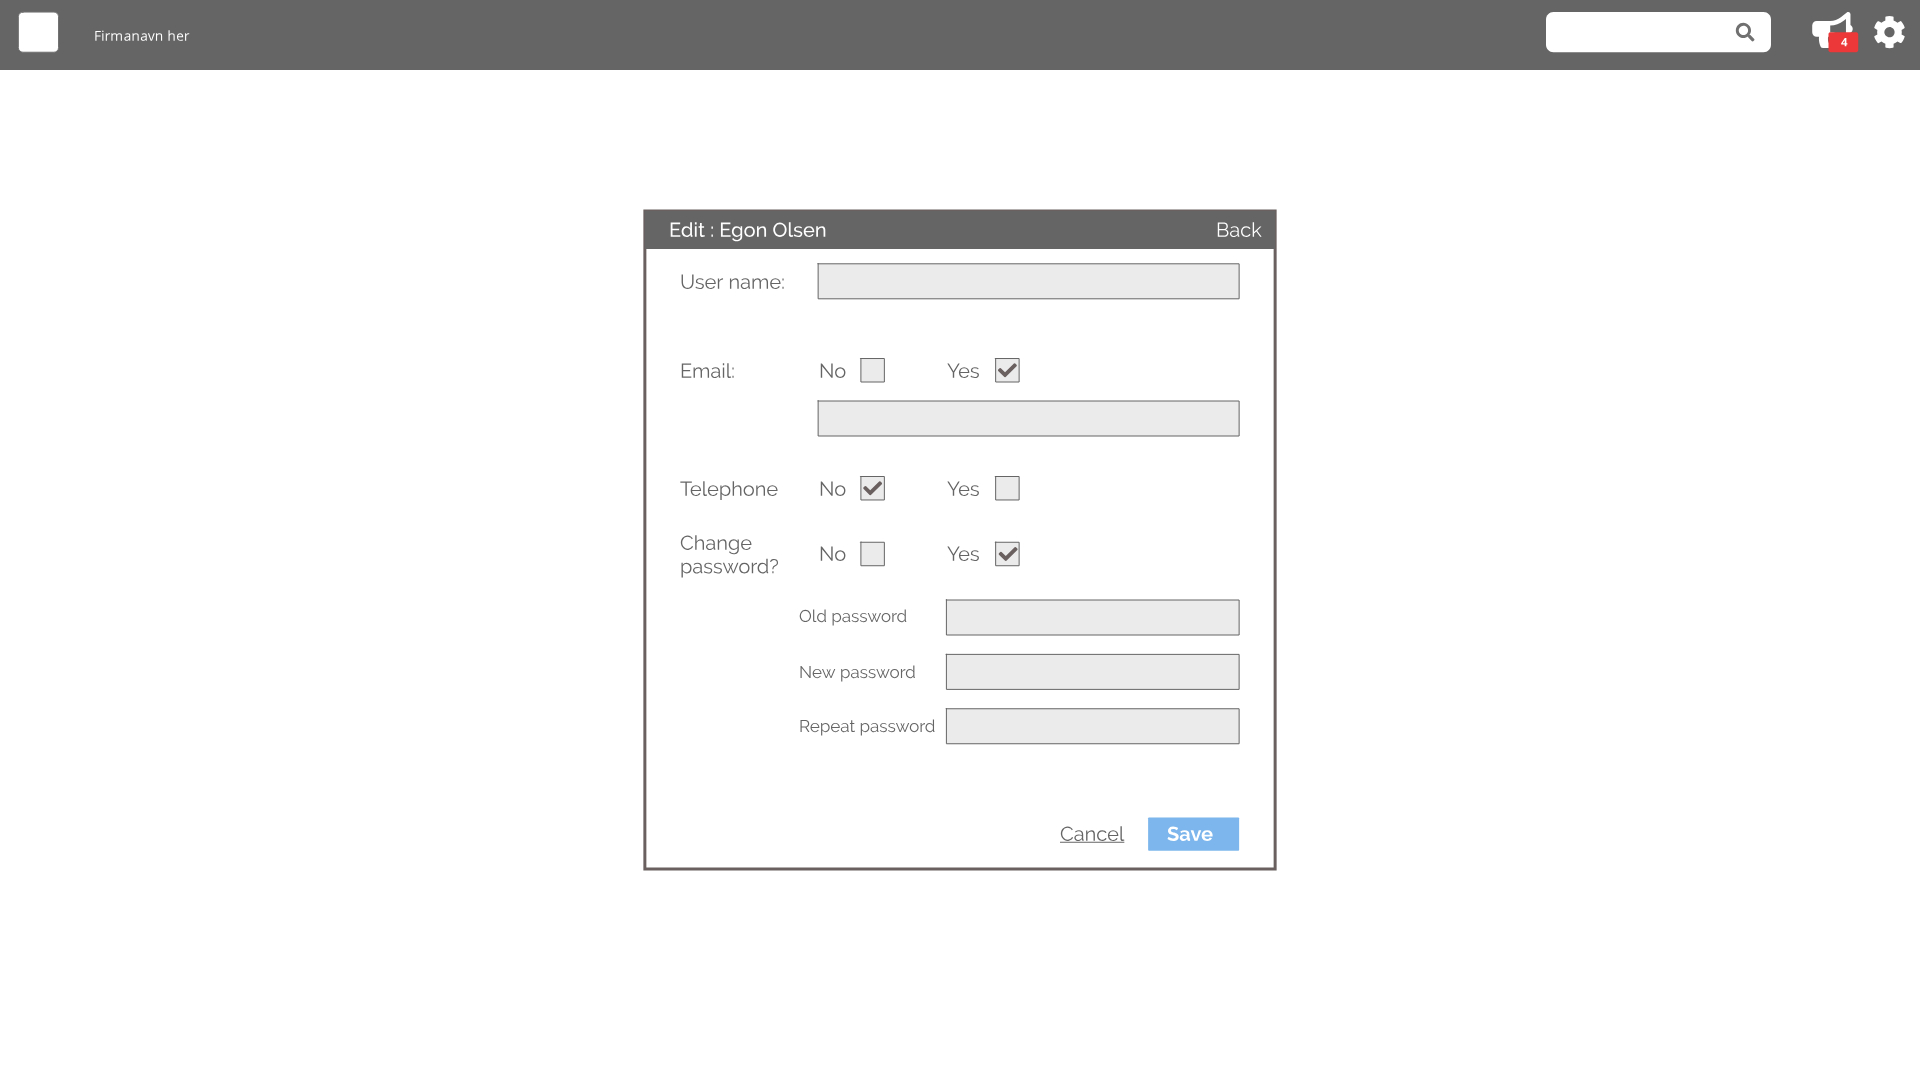
\includegraphics[width=\textwidth]{billeder/iteration3Prototyper/Page_28.jpg}
		\caption{Edit profile setting interface}
		\label{fig:5-ProfileEdit}
	\end{subfigure}
	\caption{User information interface design from mockup}\label{fig:5-UserMockUp}
\end{figure}


%Fjerde blok
\begin{figure}[H]
	\centering
	\begin{subfigure}[b]{0.48\textwidth}
		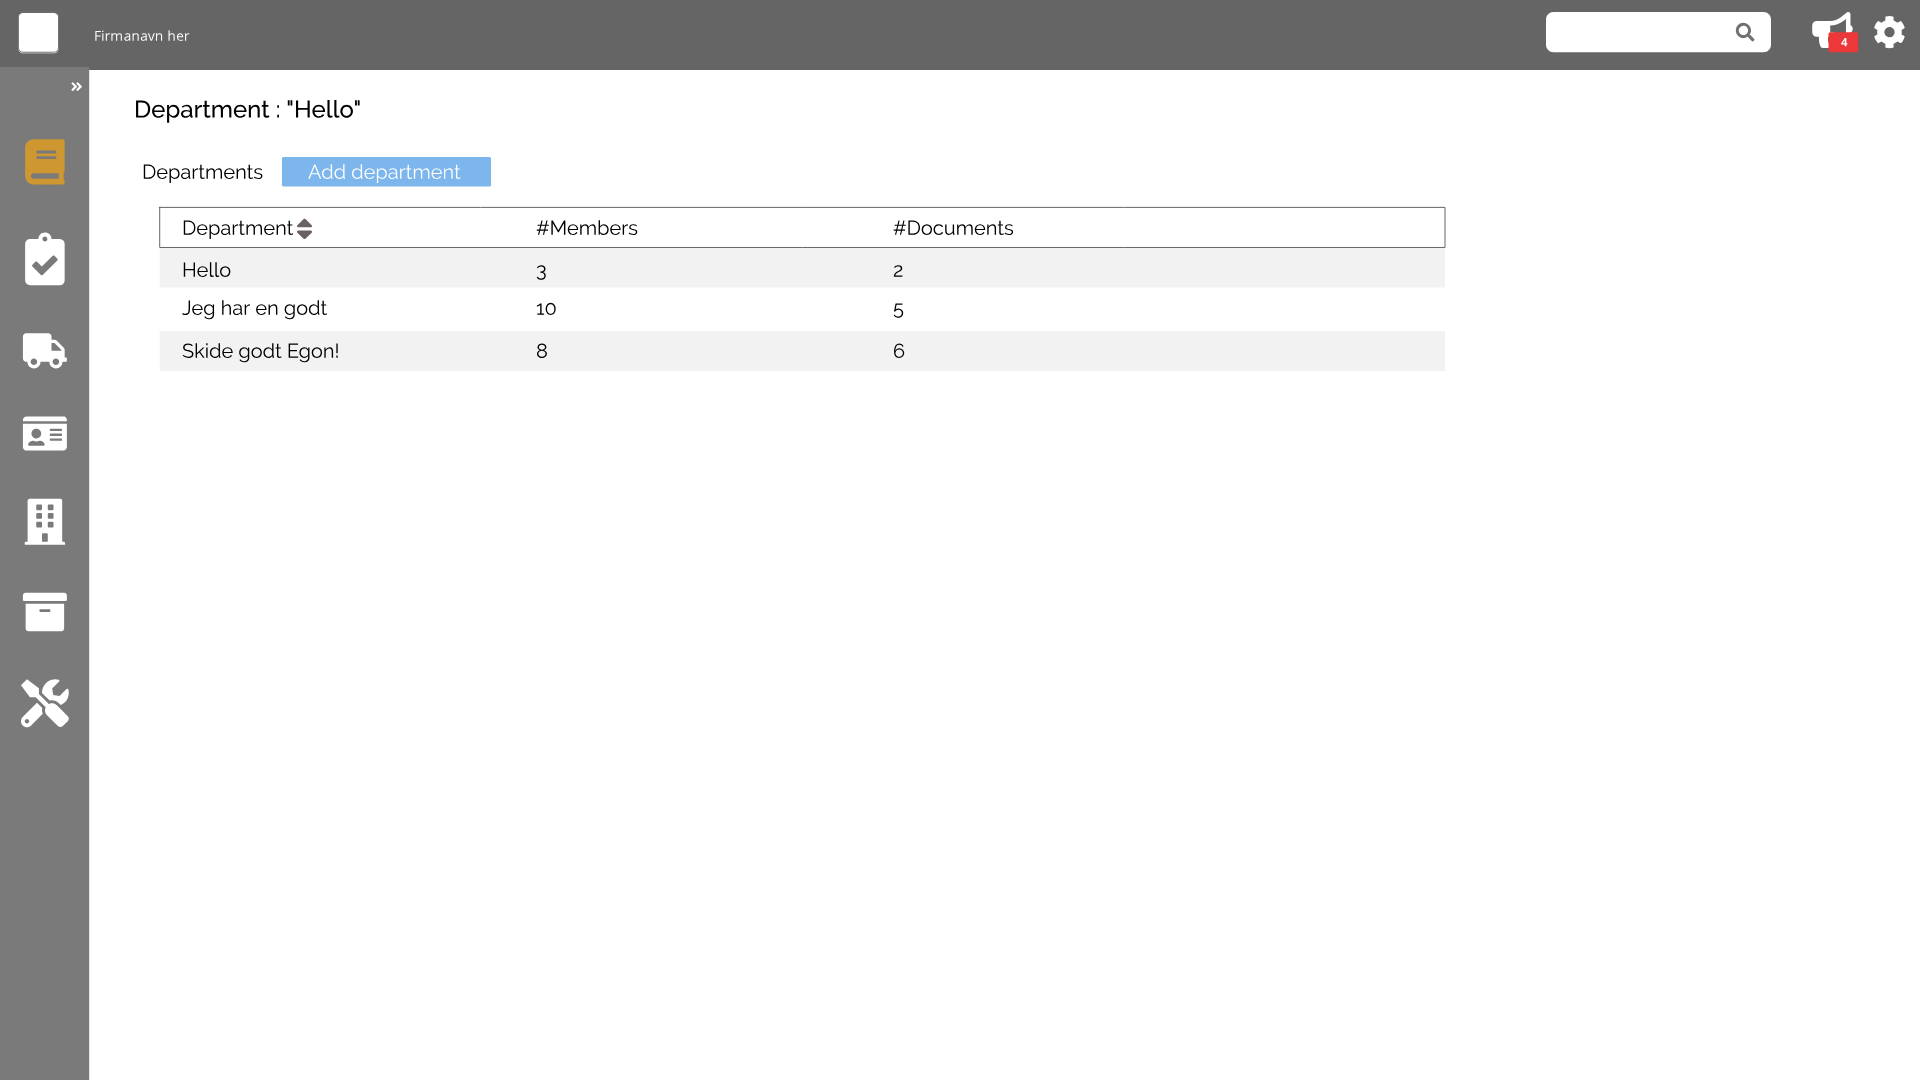
\includegraphics[width=\textwidth]{billeder/iteration3Prototyper/Page_22.jpg}
		\caption{Department main interface}
		\label{fig:5-Depart}
	\end{subfigure}
	\quad
	\begin{subfigure}[b]{0.48\textwidth}
		\includegraphics[width=\textwidth]{billeder/iteration3Prototyper/Page_24.jpg}
		\caption{Tried adding existing department interface}
		\label{fig:5-AddDepWrong}
	\end{subfigure}
\end{figure}
\begin{figure}[H]\ContinuedFloat
	\centering
	\begin{subfigure}[b]{0.48\textwidth}
		\includegraphics[width=\textwidth]{billeder/iteration3Prototyper/Page_25.jpg}
		\caption{Department detail interface}
		\label{fig:5-DepDetail}
	\end{subfigure}
	\quad
	\begin{subfigure}[b]{0.48\textwidth}
		\includegraphics[width=\textwidth]{billeder/iteration3Prototyper/Page_26.jpg}
		\caption{Department manage users and documents}
		\label{fig:5-DepEdit}
	\end{subfigure}
	\caption{Department interface design from mockup}\label{fig:5-DepMockUp}
\end{figure}

\newpage
\section{Main Interfaces From Prototype For Fifth Meeting With Ipsen}\label{sec:3prototype}
%Første blpok af billeder
\begin{figure}[H]
	\centering
	\begin{subfigure}[b]{0.48\textwidth}
		\includegraphics[width=\textwidth]{billeder/iteration3Prototyper/MainWriteAdmin.png}
		\caption{First main interface for writer and administrator}
		\label{fig:5-Main1Write}
	\end{subfigure}
	\quad
	\begin{subfigure}[b]{0.48\textwidth}
		\includegraphics[width=\textwidth]{billeder/iteration3Prototyper/MainWriteAdmin2.png}
		\caption{Second main interface for writer and administrator}
		\label{fig:5-Main2write}
	\end{subfigure}
\end{figure}
\begin{figure}[H]\ContinuedFloat
	\centering
	\begin{subfigure}[b]{0.48\textwidth}
		\includegraphics[width=\textwidth]{billeder/iteration3Prototyper/Preview.png}
		\caption{Full preview interface for writer and administrator}
		\label{fig:5-FullPreviewWrite}
	\end{subfigure}
	\quad
	\begin{subfigure}[b]{0.48\textwidth}
		\includegraphics[width=\textwidth]{billeder/iteration3Prototyper/PreviewAdmin.png}
		\caption{Prevew interface with half view for writer and administrator}
		\label{fig:5-HalfPreviewWrite}
	\end{subfigure}
\end{figure}
\begin{figure}[H]\ContinuedFloat
	\centering
	\begin{subfigure}[b]{0.48\textwidth}
		\includegraphics[width=\textwidth]{billeder/iteration3Prototyper/AccessDenied.png}
		\caption{Access denied interface for writer when trying to access unauthenticated pages.}
		\label{fig:5-AccessDenied}
	\end{subfigure}
	\caption{Main interface in common with writer and administrator}\label{fig:5-MainWriteAdmin}
\end{figure}

%Anden blok af billeder
\begin{figure}[H]
	\centering
	\begin{subfigure}[b]{0.48\textwidth}
		\includegraphics[width=\textwidth]{billeder/iteration3Prototyper/MainRead.png}
		\caption{Main interface for reader.}
		\label{fig:5-MainRead}
	\end{subfigure}
	\quad
	\begin{subfigure}[b]{0.48\textwidth}
		\includegraphics[width=\textwidth]{billeder/iteration3Prototyper/PreviewReader.png}
		\caption{Preview of document for reader.}
		\label{fig:5-PreviewReader}
	\end{subfigure}
	\caption{Main interface for reader}\label{fig:5-MainReader}
\end{figure}

%Tredje blok af billeder
\begin{figure}[H]
	\centering
	\begin{subfigure}[b]{0.48\textwidth}
		\includegraphics[width=\textwidth]{billeder/iteration3Prototyper/Archive1.png}
		\caption{Main archive interface.}
		\label{fig:5-Archive1}
	\end{subfigure}
	\quad
	\begin{subfigure}[b]{0.48\textwidth}
		\includegraphics[width=\textwidth]{billeder/iteration3Prototyper/Archive2.png}
		\caption{Detail interface of archive.}
		\label{fig:5-Archive2}
	\end{subfigure}
	\caption{Selected interfaces from archive}\label{fig:5-Archives}
\end{figure}

%Fjerde blok af billeder
\begin{figure}[H]
	\centering
	\begin{subfigure}[b]{0.48\textwidth}
		\includegraphics[width=\textwidth]{billeder/iteration3Prototyper/Ver.png}
		\caption{Add a new version.}
		\label{fig:5-Add}
	\end{subfigure}
	\quad
	\begin{subfigure}[b]{0.48\textwidth}
		\includegraphics[width=\textwidth]{billeder/iteration3Prototyper/Approve.png}
		\caption{Pending approval main interface.}
		\label{fig:5-Approve}
	\end{subfigure}
\end{figure}
\begin{figure}[H]\ContinuedFloat
	\centering
	\begin{subfigure}[b]{0.48\textwidth}
		\includegraphics[width=\textwidth]{billeder/iteration3Prototyper/AppConfirm.png}
		\caption{Confirm approval popup.}
		\label{fig:5-AppConfirm}
	\end{subfigure}
	\caption{Interfaces in connection to adding and approving a new version}\label{fig:5-Approval}
\end{figure}

%Femte blok af billeder
\begin{figure}[H]
	\centering
		\includegraphics[width=0.48\textwidth]{billeder/iteration3Prototyper/Setting.png}
		\caption{Company settings}
		\label{fig:5-setting}
\end{figure}

%Sjette blok af billeder
\begin{figure}[H]
	\centering
	\begin{subfigure}[b]{0.48\textwidth}
		\includegraphics[width=\textwidth]{billeder/iteration3Prototyper/EditU.png}
		\caption{Edit own profile information.}
		\label{fig:5-Add}
	\end{subfigure}
	\quad
	\begin{subfigure}[b]{0.48\textwidth}
		\includegraphics[width=\textwidth]{billeder/iteration3Prototyper/UserMan.png}
		\caption{User management main interface for administrator.}
		\label{fig:5-UManagement}
	\end{subfigure}
\end{figure}
\begin{figure}[H]\ContinuedFloat
	\centering
	\begin{subfigure}[b]{0.48\textwidth}
		\includegraphics[width=\textwidth]{billeder/iteration3Prototyper/EditUAdmin.png}
		\caption{Administrators edit user interface.}
		\label{fig:5-EditUAdmind}
	\end{subfigure}
	\quad
	\begin{subfigure}[b]{0.48\textwidth}
		\includegraphics[width=\textwidth]{billeder/iteration3Prototyper/Dep1.png}
		\caption{Department main interface.}
		\label{fig:5-Dep1}
	\end{subfigure}
\end{figure}
\begin{figure}[H]\ContinuedFloat
	\centering
	\begin{subfigure}[b]{0.48\textwidth}
		\includegraphics[width=\textwidth]{billeder/iteration3Prototyper/Dep2.png}
		\caption{Detail interface of a specific department}
		\label{fig:5-Dep2}
	\end{subfigure}
	 \quad
 	\begin{subfigure}[b]{0.48\textwidth}
 		\includegraphics[width=\textwidth]{billeder/iteration3Prototyper/Dep3.png}
 		\caption{Edit users in department.}
 		\label{fig:5-Dep3}
 	\end{subfigure}
	\caption{Interfaces for department and user information}\label{fig:5-DepEditU}
\end{figure}


\chapter{Usability Testing} \label{bilag:utestbilag}
The methods using to develop the test plan are based on \citep[p.~65-91]{HandbookofUsabilityTesting}. 

\section{Research questions}
The research questions are used to support observations to gain a better understanding of the test subject's point of view regarding the current state of the application. 
However it is not necessarily to be answered.

\begin{itemize}
	\item Are user able to create a document and add a version effortlessly?
	\item Does user understand the Approval functionality in the application?
	\item How well does the flow of the application reflects the expected work flow of user?
	\item How easily and successfully do user navigate through the application? 
	\item What obstacles does user meet when handling common task?
	\item Are the symbols and icons understandable and intuitive? 
	\item What are user impression of the design?
\end{itemize}

\section{Method description}
The usability testing will be perform in stages as described below.

\subsection{Session outline and timing}
The length of the test session is estimated to be one hour. The first 5 minutes will be used to introduce the test subject the usability testing structure and the think aloud principle and 20 minutes in debriefing session. 

\textbf{Introduction to the session}
Test monitor will introduce and explain to test subject how the test going to be conducted, how recording system works and the reason using these and the importance of the thinking aloud method during the test. 

\textbf{Tasks}
Test subject attempts to complete the prepared task list while test monitor observes user interaction with the application. 
Test subject has an option to ask test monitor for clarification if needed however test monitor will not help solving tasks. 

\textbf{Debriefing session}
Post-test questions will be asked to gain a better insight into user's preference and overall experience with the application. 
The debriefing session will also allow discussion to take place if desired. 

\section{Task list (First usability test)}
To be able perform a optimal usability test a task list has been prepared beforehand. 
The test subject will be asked to think aloud while solving the task.
The task list is formulated in in Danish as seen below.
 %The usability testing would be screen recorded and the test subject's interaction with the mouse and the keyboard will be recorded as well. 

Forestil dig at du arbejder som kvalitetschef hos et firma, der producerer boller. 
Du har ansvaret for firmaets håndbog og dens dokumenter. 
I firmaet er der ca. 50 medarbejdere i forskellige afdelinger, som hver især skal læse forskellige dokumenter i håndbogen. 
Det er din opgave at opdatere dokumenterne og sørge for, at de rigtige medarbejdere læser de relevante dokumenter. 
I har netop lanceret en produktion af tranebærboller.

\textbf{Setting:}
Du logger ind på systemet som administrator
På computeren i mappen “Desktop/Håndbøger” ligger “KanLauritzenLevereTranebær.pdf”  og “LauritzenKanLevereTranebær.pdf” af et dokument som skal indføres i håndbogen.

\textbf{Startup:}
\begin{enumerate}
	\item Log ind:
		\begin{itemize}
			\item Email: ips@qmsconsult.dk
			\item Kodeord: K0d30rd   (hvor 0 = nul)
		\end{itemize}

\textbf{Manage documents:}
	\item Tilføj et dokument med titlen “tranebærindkøb”. Placér det i et passende kapitel.
	\item Tilføj første version af dette dokument, “KanLauritzenLevereTranebær.pdf”-
	\item Brug dine administratorrettigheder til selv at godkende første version.
	\item Gå ind og læs dokumentet.
	\item Opdatér dokumentet med en ny version, “LauritzenKanLevereTranebær.pdf”.
	\item Sæt Egon Olsen som godkender af dette dokument og send det til godkendelse.

\textbf{Manage users \& departments:}
	\item Benny Frandsen er blevet ansat. Tilføj ham i systemet.
		\begin{itemize}
			\item Brugernavn: Benny Frandsen
			\item Email: bf@OB.dk
			\item Kodeord: K0d30rd
			\item Rolle: Reader
		\end{itemize}
	\item Tilføj en “Franz Jäger” afdeling.
	\item Tilføj Benny til “Franz Jäger” afdelingen.
	\item Tilføj dokumentet “tranebærindkøb” til “Franz Jäger” afdelingen.

\textbf{Adgang til arkivet:}
	\item I bliver nu auditeret og skal fremvise Jeres dokumentation for tranbeærindkøbene. Find dokumenterne i arkivet.
\end{enumerate}


\end{document} % Slutter dokumentet - obligatorisk
